\documentclass[12pt]{report}
\usepackage[T1]{fontenc}
\usepackage[utf8]{inputenc}
\usepackage[spanish]{babel}
\usepackage{amsmath, amsthm, amssymb, graphicx, subcaption, enumerate, hyperref, tikz, pgfplots, verbatim, pdfpages, chngcntr}
\usepackage[xindy]{glossaries}
\usepackage[algochapter]{algorithm2e}
\usepackage[autostyle]{csquotes} 

\usetikzlibrary{matrix}
%\usepackage[]{algorithm2e}
%\usepackage[top=1.5in, bottom=1.5in, left=1.5in, right=1.5in]{geometry}
%\usepackage{geometry}
 
%\addtolength{\oddsidemargin}{-.875in}
%\addtolength{\evensidemargin}{-.875in}
%\addtolength{\textwidth}{1.75in}
%\addtolength{\topmargin}{-.875in}
%\addtolength{\textheight}{1.75in}
\addtolength{\footskip}{5pt} % Para que los numeros no esten tan pegados al texto

\counterwithout{footnote}{chapter} % Footnotes con un solo conteo

%\renewcommand\figurename{Figura}
\renewcommand\spanishtablename{Tabla}
% NOTAR QUE HAY QUE PONERLE SPANISH LALA AL USAR BABEL
%\renewcommand\spanishcontentsname{\'Indice general}
\renewcommand\spanishlistfigurename{\'Indice de figuras}
\renewcommand\spanishlisttablename{\'Indice de tablas}
%\renewcommand\spanishchaptername{Cap\'itulo}
%\renewcommand\bibname{Bibliograf\'ia}
\SetAlgorithmName{Algoritmo}{algoritmo}{Lista de Algoritmos}


\newcommand{\R}{\mathbb{R}}
\newcommand{\HH}{\mathcal{H}}
\newcommand{\RR}{\mathcal{R}}
\newcommand{\signo}{\text{ signo}}
\newcommand\eq{=}
\newcommand{\minimizar}[1]{\underset{#1}{\text{minimizar}} \;}

\newtheorem{teo}{Teorema}[chapter]
\newtheorem{defn}{Definici\'on}[chapter]
\newtheorem{regla}{R}%[chapter]
\newtheorem{prop}{Proposici\'on}[chapter]
\newtheorem{cor}{Corolario}[chapter]
\newtheorem{lema}{Lema}[chapter]
\newtheorem{obs}{Observaci\'on}[chapter]
 

\makenoidxglossaries
\newglossaryentry{sesion}{
	name={Sesión},
	text={sesión},
	plural={sesiones},
	description={Una entrada a un sitio web. En cada sesión se puede ver varias páginas dentro del mismo sitio}
}
\newglossaryentry{visita}{
	name={Visita},
	text={visita},
	plural={visitas},
	description={Número de sesiones que tuvo una página web en un periodo dado}
}
\newglossaryentry{conversionrate}{
	name={Tasa de conversión},
	text={tasa de conversión},
	description={Proporción de sesiones que generan una venta sobre las sesiones totales}
}
\newglossaryentry{bouncerate}{
	name={Tasa de rebote},
	text={tasa de rebote},
	plural={tasas de rebote},
	description={Proporción de veces que las visitas a la página no generan ningún \emph{click} antes de salir}
}
\newglossaryentry{setcompe}{
	name={Set competitivo},
	text={set competitivo},
	plural={sets competitivos},
	description={El principal grupo de competidores de una compañía}
}
\newglossaryentry{r}{
	name={The R Project for Statistical Computing (\texttt{R})},
	text={\texttt{R}},
	description={Lenguaje interpretado de programación para cómputo estadístico}
}
\newglossaryentry{abtesting}{
	name={A/B Testing},
	text={A/B testing},
	description={A veces llamado \textit{split testing} consiste en comparar dos versiones de una página web para ver cuál tiene un mejor desempeño}
}
\newglossaryentry{sp}{
	name={Stored Procedure (SP)},
	text={procedimiento almacenado},
	plural={procedimientos almacenados},
	description={Procedimiento almacenado físicamente en una base de datos que se ejecuta directamente en el motor de bases de datos facilitando la integración de sistemas. Para fines prácticos es una abstracción de una consulta, que puede tener argumentos de entrada, de manera similar a una función.}
}
\newglossaryentry{sql}{
	name={Structured Query Language (SQL)},
	description={Structured Query Language (SQL): Lenguaje de programación que permite realizar consultas a bases de datos relacionales de forma estándar}
}
\newglossaryentry{sqlserver}{
	name={SQL Server},
	description={Sistema para la gestión de bases de datos producido por Microsoft basado en el modelo relacional. Sus lenguajes para consultas son T-SQL y ANSI SQL}
}


 %%%%%%%%%%%%%%%%%%%%%%%%%%%%%%%%%%%%%%%%%%%%%%%%%%%%
\begin{document}

%%%%%%%%%%%%%%%%%%%%%%%%%%%%%%%%%%%%%%%%%%%%%%%%%%%%
% PORTADA 1a HOJA IMPRESA
%\includepdf{CaratulaTesisFelipe.pdf}
\pagenumbering{gobble}
{\large
\begin{center}
INSTITUTO TECNOLÓGICO AUTÓNOMO DE MÉXICO
\end{center}
\begin{figure}[h]
 	\centering
	
\includegraphics[width=0.4\textwidth]{imagenes/logo_ITAM.jpg}
	\end{figure}
\begin{center}
\vspace{0cm}
\textbf{SISTEMA DE RECOMENDACIÓN DE HOTELES SIMILARES}\\
\vspace{1cm}
TESIS\\
\vspace{1cm}
{\normalsize QUE PARA OBTENER EL GRADO DE}\\
\vspace{0.5cm}
MAESTRO EN CIENCIA DE DATOS\\
\vspace{0.5cm}
{\normalsize PRESENTA}\\
\vspace{1cm}
FELIPE GERARD VALDÉS\\
\vspace{2cm}
{\normalsize ASESOR: M.C. NADIA DEL VILLAR}\\
\vspace{2cm}
\end{center}
\begin{flushleft}
CIUDAD DE MÉXICO\hfill 2016%\phantom{20144}
\end{flushleft}
}
 
%%%%%%%%%%%%%%%%%%%%%%%%%%%%%%%%%%%%%%%%%%%%%%%%%%%% 
% DISCLAIMER
\newpage
\noindent``Con fundamento en los artículos 21 y 27 de la Ley Federal del Derecho de Autor y como titular de los derechos moral y patrimonial de la obra titulada \textbf{`SISTEMA DE RECOMENDACIÓN DE HOTELES SIMILARES'}, otorgo de manera gratuita y permanente al Instituto Tecnológico Aut\'onomo de M\'exico y a la Biblioteca Ra\'ul Bailleres Jr., autorizaci\'on para que fijen la obra en cualquier medio, incluido el electr\'onico, y la divulguen entre sus usuarios, profesores, estudiantes o terceras personas, sin que pueda percibir por tal divulgaci\'on una contraprestaci\'o''
\vspace{40pt}
\begin{center}
\textbf{Felipe Gerard Vald\'es}\vspace{2cm}\\
\noindent\begin{tabular}{c}
\makebox[2in]{\hrulefill}\\
FECHA\vspace{2cm}\\
\makebox[2in]{\hrulefill}\\
FIRMA
\end{tabular}
\end{center}

\pagenumbering{Roman} % para comenzar la numeracion de paginas en numeros romanos


% ------------------------------------------------

\newpage
%\pagestyle{empty}  % No headers or footers for the following pages

\null\vfill
% Now comes the "Funny Quote", written in italics
\blockquote{\textit{Las empresas de tecnología, como Best Day Travel Group, deben tener en claro que el producto que manejan es la información. Los proyectos como el sistema de recomendación de hoteles similares convierten esta información en valor competitivo para mantenernos a la vanguardia en el mercado.}

\begin{flushright}
- Christian Kremers, CEO de Best Day Travel Group
\end{flushright}
}



\vfill\vfill\vfill
\clearpage



\newpage
\phantom{.}

\vspace{2cm}


{\it



\begin{flushleft}
A Felipe y Minoja, que me apoyaron más allá de lo que podría pedir.\\
Han sido una bendición en mi vida.
\end{flushleft}

\vspace{1.5cm}

\begin{flushright}
A Stéph, mi futura esposa. Jamás habría llegado a donde estoy sin tenerte de apoyo constante a mi lado. El fin de esta etapa señala el inicio de nuestra nueva vida juntos.
\end{flushright}

\vspace{1.5cm}

\begin{flushleft}
A las demás personas que hicieron esto posible como guías, editores, compañeros y amigos: Nadia, Irving y Adolfo.
\end{flushleft}

\vspace{1.5cm}

\begin{center}
$\sim$ Salmos 91 $\sim$
\end{center}

}


% ----------------------------------------------------------------------------------------------------
\tableofcontents
\listoffigures
%\listoftables

% ----------------------------------------------------------------------------------------------------
\addcontentsline{toc}{chapter}{Pr\'ologo}
\chapter*{Pr\'ologo} \label{cap:0}
\pagenumbering{arabic}

Las agencias de viajes han migrado la mayor parte de su negocio a las ventas en línea. Eso implica que junto con sus precios y la calidad de su servicio, la experiencia de usuario en sus páginas web es una parte crucial si quieren conseguir una ventaja competitiva. Dado que la mayor parte de las agencias empezaron antes de la era del Internet, el cambio al mundo digital ha sido paulatino y por necesidad, más que rápido y por gusto. Dado que el negocio consiste en \emph{vender} viajes, la primera prioridad que se tiene al hacer una página es que sea operativa. La segunda prioridad normalmente es que sea agradable a la vista y aceptablemente fácil de usar. Estos dos principios tienen mucho sentido y de hecho los portales web actuales de las agencias de viajes los siguen razonablemente bien. Sin embargo, la era del Internet es mucho más que un punto de venta en cada casa.

Sería imprudente pensar que la experiencia de comprar en casa vía electrónica es exactamente igual que comprar en un quiosco de una agencia. La diferencia clave es el conocimiento que tienen los vendedores, que está ausente en una página web. La razón por la que esto es importante es que los clientes muchas veces no saben bien lo que quieren, y mucho menos lo que hay disponible. Entonces, suponiendo que se tiene resuelta la parte estática de la página (i.e. que sea funcional, utilizable y agradable), la tercera prioridad debería ser sustituir de algún modo al vendedor. Para ello es necesario hacer que la página sea dinámica y que tome ciertas decisiones automáticamente, de modo que pueda ayudarle al cliente a encontrar (y por lo tanto a comprar) la mejor opción disponible.

Usualmente, el primer componente de las páginas web que se busca que sea inteligente es el orden en el que aparecen los hoteles cuando se busca un destino en particular, también llamado \emph{Sort Order}. La razón de esto es simple: dado que se sabe a dónde quiere ir el cliente, hay que darle las mejores opciones. Aquí el término ``mejores'' es, desde luego, desde el punto de vista del cliente, pero en última instancia lo que se busca es aumentar las ventas y la rentabilidad de la empresa. Es común que en esta parte haya filtros adicionales, como el rango de precio y la categoría del hotel (es decir, sus estrellas) que permitan al cliente refinar su búsqueda. Si bien esto funciona bastante bien, también es cierto que en un destino con muchas opciones puede seguir siendo demasiado vago y, además, obliga al cliente a ser su propio asesor. La pregunta ahora es qué más se puede hacer para incorporar información y así ayudar a cerrar ventas.

Conocer el destino del viaje del cliente es cercano a lo mínimo que se puede saber sobre él. Sin embargo, cuando se mete a la página de un hotel en particular nos proporciona bastante más información. En particular, nos da una idea de su presupuesto, de la categoría que espera que tenga su hotel y también algo de información geográfica más detallada que sólo una ciudad o zona. A menos que apliquemos un cuestionario, no tenemos otra manera de obtener más datos sobre lo que el cliente quiere, así que a lo más que podemos aspirar es a recomendar hoteles similares al que el cliente vio en primera instancia. La esperanza aquí es que si el cliente casi encontró lo que quería en la primera opción, probablemente le guste algún hotel similar cercano. Si aún así no compra, queremos que siga y siga viendo alternativas hasta que encuentre una lo suficientemente bueno. Un sistema con estas características podría jugar el papel de asesor y, de hecho, los vendedores humanos hacen algo muy similar: escuchan al cliente y proponen una opción, reciben retroalimentación y vuelven a proponer hasta que se cierra una venta o el cliente se retira.

Ahora bien, para que el sistema que hemos delineado tenga éxito, es necesario que tenga varias características. Entraremos en detalles a lo largo de la tesis, pero a hay ciertas propiedades básicas que deberá tener si planea sustituir a un vendedor:
\begin{itemize}
	\item Deberá \emph{pensar lo más parecido a un humano}, es decir, tener un concepto de similitud y cercanía entre dos hoteles lo más parecido posible al de una persona.
	\item Deberá ser \emph{inteligente y flexible} al recomendar. Es importante que proponga alternativas viables sin caer en repeticiones. Imagine el lector que un vendedor insiste en una opción que el cliente no aprueba.
	\item Deberá \emph{ser empático y atento}, o también, tomar en cuenta el presupuesto y los cambios que el cliente proponga (por ejemplo, si el cliente repentinamente está más interesado en hoteles más económicos que antes, se deberán ajustar las recomendaciones).
	\item Deberá ser \emph{ingenioso} cuando las circunstancias sean difíciles y recomendar siempre algo, aún cuando haya poco de dónde escoger.
\end{itemize}
Aunque el lector podría pensar que los adjetivos utilizados en los puntos anteriores son ambiciosos, en realidad corresponden a funciones muy básicas y perfectamente evaluables en el contexto que nos interesa. Esperamos que al final de esta lectura lo habremos convencido de que nuestro sistema en efecto es capaz de sustituir razonablemente bien a un vendedor.

En el presente trabajo desarrollaremos paso a paso un \emph{modelo de recomendación de hoteles similares} con la filosofía descrita anteriormente, hecha a la medida especialmente para las necesidades de la empresa Best Day Travel (de aquí en adelante sólo ``Best Day''). La inquietud que tuvo esta empresa por mejorar la sección de ``Hoteles Similares'' en su página fue la que llevó a la concepción de este proyecto, por lo que el objetivo siempre fue no sólo mejorar con respecto a lo que se tenía, sino también con respecto a la competencia. Debido a la naturaleza tan aplicada del proyecto, incluimos un capítulo entero dedicado a temas técnicos relacionados con la implementación particular en el sistema actual de Best Day. A continuación describimos brevemente la estructura de la tesis.

En el primer capítulo (\ref{cap:1}) describiremos el \emph{status quo} tanto de la competencia como de Best Day con el fin de aprender de lo que ya hay y así poder mejorarlo. Estos análisis nos resultaron muy útiles para establecer los objetivos de nuestro sistema.

En el segundo capítulo (\ref{cap:2}) describiremos a detalle el modelo que construimos, incluyendo las propiedades que deberá tener para que se comporte como deseamos y tembién qué medidas tomamos para solucionar cada una de las dificultades.

El tercer capítulo (\ref{cap:3}) tiene información técnica necesaria para la implementación del modelo en el escenario real de Best Day. Incluye el tratamiento de la información y las acciones a tomar en presencia de datos de mala calidad o faltantes. En pocas palabras, es la liga entre el capítulo \ref{cap:2} y el mundo real.

En el capítulo cuatro (\ref{cap:4}) hablaremos del comportamiento del modelo desde un punto de vista teórico. Es decir, veremos si las recomendaciones tienen sentido y si el nuevo sistema tiene el comportamiento que buscábamos.

Finalmente, en la primera parte del quinto capítulo (\ref{cap:5}) examinaremos el desempeño del modelo en el mundo real vía un análisis de la página de Best Day. Posteriormente concluiremos con una discusión de algunos puntos importantes sobre el sistema, sus implicaciones y algunas ideas para trabajo futuro.

% ----------------------------------------------------------------------------------------------------
\chapter{Análisis previo} \label{cap:1}

Antes de desarrollar el modelo de recomendación de hoteles similares, es conveniente analizar el \emph{status quo}\footnote{Cabe mencionar que, dado que las páginas web cambian constantemente, es muy posible que ya no sean iguales a las de la fecha en la que se realizó el análisis.}. Comenzaremos con un análisis de la competencia, con el que extraeremos información valiosa de lo que hay actualmente en el mercado, y posteriormente haremos un análisis del sistema de Best Day. El objetivo del primero es aprender de las fortalezas y debilidades de otros para enfocar nuestro trabajo de la manera más eficiente posible, mientras que el del segundo es poner a prueba a nuestro ``vendedor'' electrónico actual y así ver qué le podemos enseñar.

\section{Sistemas actuales}

Para llevar a cabo tanto los análisis de la competencia como el propio es necesario establecer qué ámbitos de los sistemas de recomendación nos interesan. Dado que el presente trabajo está enfocado en la inteligencia detrás de las elecciones y no en un aspecto estético, nos enfocaremos en los siguientes dos campos:
\begin{enumerate}
	\item La \textbf{posición dentro de la página} de las recomendaciones, con el siguiente código de relevancia:
		\begin{itemize}
			\item \textbf{Alta:} Se ve sin bajar la página y es fácil de ver.
			\item \textbf{Media:} Se tiene que bajar la página para verlo, pero hay más información relevante para la que se tenía que bajar de todos modos.
			\item \textbf{Baja:} No se ve y se puede consultar la información relevante sin llegar a las recomendaciones.
			\item \textbf{Muy baja:} Igual que la baja, pero además está hasta el final de la página.
		\end{itemize}
	\item La \textbf{forma en la que se eligen} las recomendaciones.
\end{enumerate}

Enfatizaremos en los principales competidores de Best Day, es decir: Booking, Price Travel, Expedia y Despegar. También veremos si podemos aprender algo de TripAdvisor, que aunque no es un competidor directo, vive de recomendar hoteles y de su comunidad de comentarios. Las empresas competidoras están ordenadas según nuestra evaluación de la calidad de sus sistemas de recomendación. Las ordenamos de menos a más relevantes.

\subsection*{Price Travel (pricetravel.com)}

Pusimos a Price Travel en el primer lugar de la lista porque no tiene un sistema de recomendación de hoteles similares. Cuando se busca un destino, se presentan los hoteles en el Sort Order determinado por su sistema, pero ya que se entra a la página de un hotel en particular (independientemente de cómo se llegó a esa página), no se recomienda hoteles similares ni cercanos. De hecho, la única indicación de otros hoteles es en la pestaña de mapa, en la que se pueden ver todos los cercanos en un mapa interactivo. Ni siquiera intentaremos hacer el símil de este sistema con un asesor electrónico.

\subsection*{Booking (booking.com)}

Booking es un competidor muy importante de Best Day, aunque también tiene un mercado más grande y mayor cantidad de opciones en destinos fuera de Latinoamérica, como por ejemplo en Europa. Además, es parte de Priceline Group, que tiene páginas como Kayak (\url{kayak.com}) y a OpenTable (\url{opentable.com}). Antes de entrar en los puntos de interés general, cabe mencionar que algo que hace Booking que no hacen los demás es que cuando se busca un hotel en la página con la barra inteligente, en lugar de ir directamente a su página, se muestra en el primer lugar de una lista, dando la posibilidad de elegir algún otro hotel. Ahora sí pasemos al tema en cuestión:
\begin{itemize}
	\item \textbf{Hoteles populares por destino}
	\begin{enumerate}
		\item Se encuentran del lado izquierdo, abajo de la barra de búsqueda y fechas, como se puede ver en la figura (\ref{fig:booking:website}). Es una posición de prominencia media-baja, puesto que no es visible inmediatamente sin bajar en la página.
		\item Cuando se entra a la página (no al hotel en particular) por primera vez y se selecciona un hotel, aparece una sección de hoteles populares en el mismo destino del hotel buscado. El tema es que siempre aparece la misma selección para cada destino, independientemente del hotel que se haya elegido, pues la popularidad de los otros hoteles no tiene relación con el hotel elegido.
	\end{enumerate}
	\item \textbf{Búsquedas recientes}
	\begin{enumerate}
		\item Se encuentran en el mismo lugar que los hoteles populares por destino, pero los sustituyen una vez que se ha visitado al menos un hotel anteriormente.
		\item La información de los hoteles visitados se va almacenando en una \emph{cookie}, de modo que para los hoteles subsecuentes, en lugar de los hoteles populares por destino, aparece un listado de unos pocos hoteles recientemente buscados por el usuario.
	\end{enumerate}
\end{itemize}

%%%%%%%%%%%%%%% BOOKING
\shorthandoff{<>}
\begin{figure}[ht]
	\centering
	\begin{tikzpicture}[xscale = 2, yscale = 2]
		\fill [blue, opacity=0.2] (0,0) rectangle (2.6,2.2);
		\fill [blue, opacity=0.2] (0.2,1) rectangle (0.8,2);
		\fill [blue, opacity=0.2] (1,0.2) rectangle (2.4,2);
		\fill [red, opacity=0.5] (0.2,0.2) rectangle (0.8,0.8);
	\end{tikzpicture}
	\caption{Posición de las recomendaciones de \texttt{booking.com} (rojo) \label{fig:booking:website}}
\end{figure}
\shorthandon{<>}

Al parecer en Booking sólo están interesados en lo que el cliente ha buscado y utilizan los hoteles populares por destino para no dejar vacía la sección para los clientes nuevos. El problema con los hoteles populares por destino es que no varían según el hotel buscado (siempre y cuando estén en el mismo destino), mientras que el de las búsquedas recientes es que no promueven que el cliente explore la página y encuentre la mejor opción para sus necesidades. Podríamos comparar este sistema con un vendedor que propone una lista de hoteles primero y luego únicamente dice ``a usted le habían gustado los hoteles $x$, $y$ y $z$''. Sin duda esto es mejor que nada, pero veremos más adelante que se puede hacer bastante más.

\subsection*{Despegar (despegar.com)}

Despegar es un competidor más directo y con un mercado más parecido al de Best Day que Booking debido a que está dirigida al mercado latinoamericano (sus oficinas centrales están en Argentina). En en su página utilizan varias estrategias distintas para recomendar, por lo que las describiremos por separado. La distribución de la página está ilustrada en la figura (\ref{fig:despegar:website}). Cabe mencionar que no usan todas las estrategias para todos los hoteles, ni siempre, por lo que sospechamos que tienen información incompleta y sólo muestran lo que tienen disponible.
\begin{itemize}
	\item \textbf{Búsquedas recientes}
	\begin{enumerate}
		\item Se encuentra en la izquierda abajo del mapa. Igual que en booking.com, se tiene que bajar en la página para verlo, por lo que su relevancia es media-baja.
		\item Son los hoteles buscados recientemente por el usuario. Curiosamente, no siempre nos aparecieron al hacer búsquedas, incluso después de haber visto varios hoteles. Pensamos que esto podría deberse a alguna especie de \gls{abtesting}\footnote{Ver glosario.}.
	\end{enumerate}
	\item \textbf{Hoteles cercanos}
	\begin{enumerate}
		\item Se encuentra directamente debajo de las búsquedas recientes.
		\item Se listan los hoteles más cercanos al hotel en buscado, sin ningún criterio de precio, categoría o estilo del hotel.
	\end{enumerate}
		\item \textbf{Hoteles populares por destino}
	\begin{enumerate}
		\item Se encuentra directamente abajo de los hoteles cercanos.
		\item Para cada destino muestra una lista de los hoteles más populares (presumiblemente los más vendidos). La lista es la misma para todos los hoteles en un destino dado y de hecho contiene al hotel buscado en su posición correspondiente (es decir ni se omite ni aparece hasta arriba).
	\end{enumerate}
	\item \textbf{Otros usuarios también buscaron...}
	\begin{enumerate}
		\item Aparece en la parte inferior de la página, abajo de prácticamente todo. Su relevancia es muy baja y de hecho se omitió en los primeros análisis de la competencia porque no lo vimos.
		\item En la parte inferior de la página también aparece una sección de hoteles que fueron visitados por los demás usuarios que han visto el hotel en cuestión. Este análisis no es complejo, pero puede ser pesado computacionalmente si no se utiliza un  método apropiado.
	\end{enumerate}
\end{itemize}

%%%%%%%%%%%%%%% DESPEGAR
\shorthandoff{<>}
\begin{figure}[ht]
	\centering
	\begin{tikzpicture}[xscale = 2, yscale = 2]
		\fill [blue, opacity=0.2] (0,-0.6) rectangle (2.6,2.2);
		\fill [blue, opacity=0.2] (0.2,1.4) rectangle (0.8,2);
		\fill [blue, opacity=0.2] (1,0.2) rectangle (2.4,2);
		\fill [green, opacity=0.5] (0.2,0.8) rectangle (0.8,1.2);
		\fill [red, opacity=0.5] (0.2,0.2) rectangle (0.8,0.6);
		\fill [white, opacity=0.5] (1,-0.4) rectangle (2.4,0);
	\end{tikzpicture}
	\caption{Distribución de \texttt{despegar.com}. Se muestran los hoteles cercanos (verde), los populares por destino (rojo) y los elegidos por otros usuarios (blanco) \label{fig:despegar:website}}
\end{figure}
\shorthandon{<>}

En Despegar tuvieron muchas ideas para recomendar, pero todos los criterios están separados y no colaboran entre sí. Es como tener una tabla ordenada por varios campos distintos. Los hoteles recomendados con base en lo que han visto otros clientes creemos que están desperdiciados en donde están, puesto que sólo los clientes que vayan hasta abajo de la página los verán. El sistema funciona razonablemente bien y permite movilidad hacia arriba en la categoría del hotel. El problema es que es claramente sesgado a recomendar hoteles populares, de modo que tiende a atorarse en aglomerados de hoteles populares y también a subir de categoría. El resultado es que después de algunos pocos \emph{clicks}, casi invariablemente se llega a los hoteles más caros de la zona, sin posibilidad de explorar otros.

La ventaja de Despegar es que al menos toman en cuenta que hay diversos criterios de interés. El problema es que su ``vendedor'', o es incapaz de integrar varios criterios, o bien insistente, poco creativo y además nos quiere vender lo más caro que se pueda. Sin duda es mejor que el de Booking, pero aún podría mejorar bastante.

\subsection*{Expedia (expedia.com)}

Expedia es otra agencia de viajes que está invirtiendo mucho en entrar al mercado mexicano con sus marcas \url{expedia.com} y \url{hoteles.com}. Además, es una de las agencias que más énfasis está poniendo en los sistemas inteligentes. De hecho, tienen un sistema diferente a los demás y por eso lo pusimos en esta posición en la lista de sistemas competidores, aunque por alguna razón, en su página las recomendaciones están posicionadas en un lugar casi imposible de ver, como se puede ver en la figura (\ref{fig:expedia:website}). 
\begin{itemize}
	\item \textbf{Búsquedas recientes}
	\begin{enumerate}
		\item Se encuentran en el centro, casi hasta abajo, después de toda la información del hotel. La prioridad es muy baja.
		\item Es igual que en las demás páginas. Aparecen los últimos cuatro hoteles buscados distintos del actual (en caso de repetir una búsqueda).
	\end{enumerate}
	\item \textbf{Hoteles recomendados}
	\begin{enumerate}
		\item Se encuentran directamente abajo de las búsquedas recientes.
		\item Utilizan un método desconocido para recomendar hoteles similares que permite movilidad progresiva entre categorías. No estamos seguros si tiene alguna restricción de precios.
	\end{enumerate}
\end{itemize}

%%%%%%%%%%%%%%% EXPEDIA
\shorthandoff{<>}
\begin{figure}[ht]
	\centering
	\begin{tikzpicture}[xscale = 2, yscale = 2]
		\fill [blue, opacity=0.2] (0,-0.6) rectangle (2.6,2.2);
		\fill [blue, opacity=0.2] (0.2,0.8) rectangle (0.8,2);
		\fill [blue, opacity=0.2] (1,0.8) rectangle (2.4,2);
		\fill [white, opacity=0.5] (1,-0.4) rectangle (2.4,0);
		\fill [red, opacity=0.5] (1,0.2) rectangle (2.4,0.6);
	\end{tikzpicture}
	\caption{Posición de las recomendaciones de \texttt{expedia.com}. Se muestran los hoteles vistos (blanco) y las recomendaciones (rojo)\label{fig:expedia:website}}
\end{figure}
\shorthandon{<>}

El sistema de recomendación de Expedia nos gustó bastante y de hecho creemos que está siendo desaprovechado. Permite explorar los hoteles disponibles hacia arriba y hacia abajo en la escala de precio y categoría y llegar a opciones completamente nuevas. Una ventaja sobre el algoritmo de Booking es que no tiene una tendencia tan fuerte hacia los hoteles caros. En cuanto a las desventajas, es probable que esté acotado por destino, aunque eso no es tan grave. Otro detalle que no nos convenció es que le falta algo de flexibilidad: después de seleccionar algunas pocas recomendaciones, es evidente que nunca saldremos de un cierto grupo de hoteles.

En conclusión, creemos que el enfoque que tomó Expedia es el correcto, puesto que emulan un vendedor que, por un lado, propone nuevas alternativas y, por otro, se ``acuerda'' de lo que ya le había gustado al cliente. Lo que le faltaría es ser menos tímido (i.e. poner las recomendaciones en un lugar de mayor impacto) y menos conservador (i.e. proponer opciones que se salgan de un círculo reducido de hoteles).

\subsection*{Trip Advisor (tripadvisor.com)}

Como decíamos arriba, Trip Advisor no es la competencia directa de Best Day, pero es un sitio muy popular de evaluación de hoteles y creemos que podemos aprender de ellos.
\begin{itemize}
	\item \textbf{Hoteles similares}
	\begin{enumerate}
		\item Se encuentran en la derecha, abajo de la foto principal, pero al lado de otra información importante, por lo que el impacto es medio (ver figura (\ref{fig:tripadvisor:website})).
		\item No sabemos cómo hacen las recomendaciones, pero no son por distancia estricta y sí permiten cierta movilidad de la categoría.
	\end{enumerate}
\end{itemize}

%%%%%%%%%%%%%%% TRIP ADVISOR
\shorthandoff{<>}
\begin{figure}[ht]
	\centering
	\begin{tikzpicture}[xscale=2, yscale = 2]
		\fill [blue, opacity=0.2] (0,-0.6) rectangle (2.6,2.2);
		\fill [blue, opacity=0.2] (0.2,0.8) rectangle (2.4,2);
		\fill [blue, opacity=0.2] (0.2,-0.4) rectangle (1.4,0.6);
		\fill [red, opacity=0.5] (1.6,-0.4) rectangle (2.4,0.6);
	\end{tikzpicture}
	\caption{Posición de las recomendaciones de \texttt{tripadvisor.com} (rojo)\label{fig:tripadvisor:website}}
\end{figure}
\shorthandon{<>}

El sistema de TripAdvisor también funciona razonablemente bien, pero parece estar más basado en la calificación de los usuarios que en la categoría del hotel. Nos pareció que podría mejorar si tuviera una mayor flexibilidad, pues comparte el problema de la falta de inventiva del sistema de Expedia. A pesar de las faltas, este enfoque tiene sentido en el contexto de su página y funciona más o menos bien.

Es posible que el sistema de TripAdvisor sea un filtro colaborativo, como por ejemplo el de \cite{mmds}, desde el punto de vista de los productos (i.e. \emph{item-based}). Un sistema de este estilo podría funcionar bien si se tuviera clientes recurrentes\footnote{Un cliente recurrente es uno que ha comprado al menos dos veces.}, puesto que está basado en hacer silogismos del tipo ``a los clientes que les gustó A también les gustó B''. Sin embargo, Best Day no tiene una recurrencia tan alta (es decir, tiene muchos clientes que han comprado una sola vez) y tampoco tiene información suficientemente detallada de los clientes como para tratar de seguir por este camino. Por lo tanto, sería inviable implementar un sistema de este estilo.


\subsection*{Best Day (bestday.com.mx)}

Finalmente, analizaremos lo que se hace actualmente en Best Day. Del mismo modo que con la competencia, comenzaremos con una breve descripción; la distribución está ilustrada en la figura (\ref{fig:bestday:website}).
\begin{itemize}
	\item \textbf{Hoteles similares}
	\begin{enumerate}
		\item Los hoteles similares están abajo de la liga al mapa del lado derecho. Como en la mayoría de los competidores, no se ve inmediatamente al entrar en la página, por lo que tiene prominencia media-baja.
		\item La manera de recomendar hoteles es por categoría (estrellas) y por destino, es decir, se toman los hoteles de las mismas estrellas y en el mismo destino que el hotel buscado y se presentan en el Sort Order del momento. No se toma en cuenta el precio ni la distancia (salvo por el hecho de encontrarse en el mismo destino) de las opciones.
	\end{enumerate}
	\item \textbf{Búsquedas recientes}
	\begin{enumerate}
		\item Se encuentran directamente debajo de los hoteles similares.
		\item Similarmente a la competencia, aparece una lista de los hoteles que el usuario visitó recientemente. Las búsquedas recientes permanecen entre \glspl{sesion} dentro de una misma computadora, utilizando \emph{cookies}.
	\end{enumerate}
\end{itemize}

%%%%%%%%%%%%%%% BEST DAY
\shorthandoff{<>}
\begin{figure}[ht]
	\centering
	\begin{tikzpicture}[xscale = 2, yscale = 2]
		\fill [blue, opacity=0.2] (0,0) rectangle (2.6,2.2);
		\fill [blue, opacity=0.2] (0.2,0.2) rectangle (1.6,2);
		\fill [blue, opacity=0.2] (1.8,1) rectangle (2.4,2);
		\fill [red, opacity=0.5] (1.8,0.2) rectangle (2.4,0.8);
	\end{tikzpicture}
	\caption{Posición de las recomendaciones de \texttt{bestday.com} (rojo)\label{fig:bestday:website}}
\end{figure}
\shorthandon{<>}

Sin duda, el hecho de tener una sección de búsquedas recientes es un punto a favor de este sistema de recomendación, aunque no aporta nada que no tengan los competidores. Desafortunadamente, la calidad de sus recomendaciones es muy variable. En zonas homogéneas y con mucha oferta para una categoría dada, las recomendaciones pueden ser aceptables. Sin embargo, en destinos donde hay hoteles muy distintos pero con la misma categoría, como podrían ser un hotel citadino y uno de playa, las recomendaciones dejan mucho que desear. Además, si no hay hoteles bajo este criterio, o si hay muy pocos, no se muestra nada, o una lista muy pequeña. Es decir, el ``asesor'' electrónico de Best Day maneja las recomendaciones en grupos: dada información del cliente (destino y estrellas) es sumamente insistente con las alternativas. En pocas palabras, no tiene ninguna ventaja sobre un catálogo agrupado por destino y estrellas.

\section{Diagnóstico}

En los siguientes párrafos resumiremos lo que aprendimos del análisis de la competencia y del estado actual de Best Day. En primer lugar, nos dimos cuenta de que poner una sección con las búsquedas recientes es algo muy deseable y relativamente fácil de implementar. De hecho, es un estándar en la industria, pues todos los competidores lo tienen, a excepción de Price Travel. Sin duda es deseable que un vendedor recuerde los artículos que le ha mostrado al cliente, aunque esto de ninguna manera es suficiente para crear una sensación de inteligencia.

Quitando las búsquedas recientes de en medio, podemos analizar los diversos sistemas de recomendación. Un punto que pensamos que es sumamente importante es el precio. Hasta donde pudimos ver, ninguna página tiene miramiento alguno con el costo de los hoteles recomendados. El resultado es que pueden recomendar hoteles del doble o incluso triple de precio que el original. Creemos que esto no promueve que el cliente explore más alternativas, ya que la mayoría basa su decisión fuertemente en el precio de los hoteles. Para ver que tomar el precio en cuenta es importante, basta imaginar que un vendedor en una tienda nos intenta vender artículos más y más caros. Sin duda es molesto y menos agradable que uno que busca encontrar productos que satisfagan nuestras necesidades sujeto a nuestras restricciones presupuestales. Propondremos una forma simple de lidiar con este problema sin perder demasiada flexibilidad en las recomendaciones.

Otro factor que nos pareció mejorable es el uso de la información geográfica. Parece ser que la opción más popular es únicamente utilizar la información incluida en el destino y, de hecho, parece que sólo Despegar tiene una sección de hoteles más cercanos. Si bien utilizar el destino como punto de partida es una opción razonable, creemos que se podría aprovechar mejor la información si se utilizaran las coordenadas geográficas, dado que en la vida real lo que realmente importa es la proximidad de los hoteles; los destinos son particiones más o menos arbitrarias que no deberían afectar mucho las recomendaciones. Por ejemplo, una persona podría recomendar un hotel en Cancún dado que se buscó uno en la zona norte de la Riviera Maya, o uno en Playa del Carmen a una persona que buscó algo en Cozumel.

Un tercer problema con el que nos encontramos en las recomendaciones es que en la mayoría de los casos eran estáticas. Es decir, son idénticas para ciertos grupos de hoteles. Esto pasa en todas las opciones que vimos que utilizan el destino (Booking, Despegar, Best Day) como criterio, pues no dependen también del hotel. Esto en sí mismo puede ser un problema en destinos amplios, puesto que el usuario agota las opciones rápidamente. Hay que decir que de ninguna manera decimos que las recomendaciones estáticas son malas, pero su función debe ser desempeñada por catálogos o por búsquedas avanzadas, no por sistemas de recomendación.

En cuarto lugar, nos dimos cuenta que en varias de las páginas utilizan diversos criterios para recomendar hoteles, pero muchas veces no los han integrado. La estrategia tiende a ser usar un criterio para ordenar a la vez, en lugar de aprovechar varios simultáneamente. Este punto va de la mano con el tercero: los criterios estáticos deben ir en una búsqueda avanzada. Es necesario integrarlos de alguna forma para que parezcan, aunque sea de lejos, inteligentes.

En quinto lugar, notamos que en general los sistemas que sí recomendaban de forma más sofisticada resultaban rígidos y se podían quedar atorados fácilmente en grupos aislados de hoteles. Esto hace que el sistema se vuelva inútil una vez que se llegó a uno de estos grupos absorbentes. El único que nos pareció decente en este sentido es el de Expedia, aunque sí es algo más rígido de lo que nos gustaría. No podemos dejar de enfatizar la importancia que tiene la ``creatividad'' en este tipo de sistemas. De igual modo que los vendedores reales, el valor que aportan reside en sus ideas, su inventiva y sus propuestas innovadoras. Es por ello que si se les agotan las ideas (o en este caso, si se ciclan en un grupo de ellas que no sea lo suficientemente bueno) se vuelven obsoletos.

Otro punto sobre los sistemas en general, pero de los de hoteles similares en particular, es que en ninguna página (salvo tal vez Trip Advisor) aparecen en posiciones de importancia alta. En el mejor de los casos aparecen una página abajo de la principal, al lado, y en los peores casos están hasta abajo. Creemos que se está desaprovechando mucho el potencial de dichos sistemas. Es un hecho que los vendedores tímidos no son tan efectivos como podrían. En este caso es posible hacer que todos los ``vendedores'' se vuelvan instantáneamente tan extrovertidos como se desee; creemos que se debería aprovechar esta capacidad. No se trata de hacerlos intrusivos ni exagerados, pero sí de darles las herramientas (la exposición) que requieren para hacer mejor su trabajo.

Finalmente, un problema particular del sistema de Best Day es que no toma en cuenta de ninguna forma el perfil del hotel. Como mencionamos arriba, no es lo mismo un hotel de playa de cuatro estrellas que un hotel de ciudad de cuatro estrellas, y si por alguna razón ambos están en el mismo destino, como puede suceder en ciudades cerca del mar, por ejemplo, el sistema de recomendación por destino y estrellas puede fallar catastróficamente. Tenemos ejemplos de hoteles de negocios en Cancún para los que se recomienda hoteles todo incluido en la zona hotelera. Esto no es viable y claramente es importante que el algoritmo que desarrollemos tome en cuenta el perfil de los hoteles, sobre todo porque busca recomendar hoteles \emph{similares} de una manera similar a lo que haría un experto.

% ----------------------------------------------------------------------------------------------------
\chapter{Sistema de recomendación de hoteles} \label{cap:2}

En el capítulo anterior analizamos los sistemas de recomendación que tienen actualmente tanto Best Day como su competencia y expusimos los principales puntos débiles que encontramos. Ahora podemos utilizar el conocimiento obtenido para generar un sistema nuevo que tenga un mejor desempeño y propiedades más deseables que los que vimos. Primero describiremos punto por punto qué nos gustaría que hiciera el sistema y posteriormente dedicaremos una sección para profundizar en cómo resolvimos cada uno de los problemas.

\section{Modelo propuesto}

Proponemos las siguientes medidas con el fin de propiciar que las recomendaciones tengan un carácter más parecido al de un verdadero vendedor:
\begin{enumerate}
	\item Con el fin de que sea \emph{empático}, pondremos una cota superior al \textbf{precio} de los hoteles recomendados, como un porcentaje del precio del hotel buscado.
	\item Para que tome en cuenta la distancia \emph{lo más parecido posible a una persona}, proponemos que recomiende hoteles razonablemente \textbf{cercanos} al buscado, donde el criterio de cercanía varía según la densidad de hoteles en la zona.
	\item Para que \emph{compare hoteles como un vendedor}, las recomendaciones deberán tener un \textbf{perfil} o filosofía similar al original. Además, las recomendaciones deben ser hoteles no necesariamente de las mismas estrellas, pero sí deben tener una cantidad similar de \textbf{servicios} disponibles.
\end{enumerate}
En la lista anterior aparentemente hemos dejado fuera las características de \emph{ingenio} y de \emph{flexibilidad}. Sin embargo, más adelante en este capítulo y en el capítulo \ref{cap:3} veremos qué hicimos para tratar con casos atípicos o con muy poca población. Por otro lado, en el capítulo \ref{cap:4} quedará claro que el sistema propuesto naturalmente genera una estructura diversa que difícilmente se quedará enfrascada en unas pocas opciones.

Antes de entrar a una descripción detallada de cada medida, explicaremos brevemente cómo colaborarán a que nuestro sistema de recomendación tenga las propiedades que buscamos.

Siempre y cuando dos hoteles sean genuinamente similares a los ojos de una persona, la vasta mayoría de los clientes siempre preferirá el más económico. Acotando el precio esperamos que rara vez aparezcan hoteles más allá de las posibilidades del cliente en las recomendaciones. Esto contribuirá a que el sistema sea \emph{empático} porque tendrá en cuenta el presupuesto del cliente y se ajustará conforme éste explore alternativas de precios distintos.

En cuanto a la distancia entre hoteles, creemos que utilizar la distancia al hotel en cuestión es mucho más razonable que usar el mismo criterio del destino para todos, puesto que promoverá hoteles cercanos además de parecidos en otros sentidos. Dado un hotel en un mapa, una \emph{persona} naturalmente se fijaría en la distancia en línea recta a las alternativas, no utilizaría las fronteras arbitrarias de los destinos.

Esperaríamos que las similitudes de perfil y servicios trabajen conjuntamente con el criterio de cercanía para obligar a que las recomendaciones varíen de hotel a hotel, incluso dentro de un mismo destino. La ventaja de esto es que se puede explorar muchas opciones sin tener que buscar nada explícitamente, puesto que las recomendaciones abren nuevas alternativas por sí solas. Es importante que demos suficiente flexibilidad al método para que no sea rígido y no se estanque en grupos reducidos de hoteles. Estos dos criterios en su conjunto contribuiran tanto a que el ``asesor'' \emph{compare} como una persona, como a que sea \emph{creativo}.

Como último punto, no queremos utilizar estos criterios de forma aislada, pues cada uno tiene diversas faltas. Lo que queremos es integrarlos todos en un sistema poderoso que haga las veces del vendedor, es decir, que evite que el cliente tenga que pensar demasiado y que genuinamente le proponga alternativas interesantes. Para ello generaremos una medida de similitud entre los hoteles y mostraremos los más parecidos que estén a una distancia y precio razonables del hotel original. En las siguientes secciones describiremos cada uno de los criterios con mayor nivel de detalle.

Para facilitar la exposición le daremos nombres a los hoteles que van superando cada etapa, hasta llegar a las recomendaciones para cada hotel.
\begin{defn}[Conjunto de hoteles]
Denotamos el conjunto de todos los hoteles por $\HH$ y al número de hoteles por $N$, es decir $N = |\HH|$.
\end{defn}

\section{Precio}

Dado que el precio es un factor determinante en la elección de un hotel para la mayoría de los clientes, es importante respetar sus posibilidades económicas a la hora de recomendar nuevas opciones. Es razonable pensar que dados dos hoteles idénticos, un cliente siempre elegirá el más barato, salvo tal vez unos pocos clientes \emph{upscale}. Por esta razón, decidimos no imponer ninguna cota inferior al precio de los hoteles recomendados, siempre y cuando cumplan los criterios de similitud que describiremos más adelante. Por otro lado, como puede ser desalentador que las sugerencias contengan opciones demasiado caras, optamos por poner una cota superior al precio de los hoteles. Como en este paso queremos reflejar los precios ``reales'' de los hoteles, utilizaremos su precio de largo plazo para generar el filtro, como se explica a continuación.
\begin{regla}[Filtro de precio de largo plazo] \label{r:preciolargo}
Sea $\gamma \geq 0$ y sea
\[
p^D_i = \frac{\text{Importe total del hotel $i$ en el periodo $D$}}{\text{Total de noches del hotel $i$ en el periodo $D$}}
\]
el precio de largo plazo del hotel $i$ en el periodo $D$. Entonces definimos la cota superior de precio para $i$ por $(1 + \gamma)p^D_i$, es decir, excluimos del análisis para $i$ todos los hoteles $j$ con $p^D_j > (1 + \gamma)p^D_i$. Los hoteles restantes están contenidos en el conjunto
\[
\HH_i^1 = \{j \in \HH : p^D_j \leq (1 + \gamma)p^D_i\}
\]
\end{regla}
El parámetro $\gamma$ es esencialmente el porcentaje por encima del precio de $i$ que se permitirá que tengan las recomendaciones. Por ejemplo, si $\gamma = 0.3$, entonces se ignoran todas las opciones que sean más de 30\% más caras que $i$. El periodo $D$ debe ser suficientemente largo para que refleje los precios promedio de un hotel, pero no tanto como para que se vea demasiado afectado por la inflación y otros factores. Una buena elección es por ejemplo un año o dos años, pues así además se toma en cuenta los cambios de precios en las diversas temporadas del año. Cabe notar que en esta versión del modelo, tanto $\gamma$ como $D$ son los mismos para todo hotel $i$.

En pruebas empíricas nos gustó el desempeño de $\gamma$ alrededor de 0.3, ya que permite suficiente flexibilidad en los precios y las categorías sin proponer opciones excesivamente costosas.

\section{Distancia: filtro estático}

Antes de entrar en criterios dinámicos de distancia y en similitudes de hoteles, es importante pensar si su cálculo es factible. El tema es que, si bien en teoría sería suficiente calcular las similitudes de los hoteles y luego quedarnos con los cercanos, en la práctica esto es complicado. Cuando se quiere conocer la distancia entre cualesquiera dos hoteles de entre, supongamos, $N$ opciones, es necesario almacenar $(N^2 - N)/2$ números (una de las porciones triangulares de la matriz de distancias, quitando la diagonal). Para $N$ incluso moderadamente grande, la cantidad de información a guardar se vuelve prohibitiva. Para empeorar las cosas, los criterios de similitud que desarrollaremos más adelante no son simétricos, por lo que tendríamos que almacenar toda la matriz (menos la diagonal), lo que resultaría en $N^2 - N$ números.

El problema con lo anterior es que además la gran mayoría de los cálculos se desperdiciarían, ya que en nuestro contexto no tiene mucha utilidad guardar la similitud entre un hotel en Veracruz y otro en Las Vegas. Una manera de resolver este problema es ignorar hoteles que seguro no recomendaremos. Dado que queremos que el sistema regrese hoteles similares \emph{y} cercanos, es razonable ignorar los que estén más lejos que una cantidad fija suficientemente grande en cualquier destino.

Hay diversas fórmulas para calcular la distancia entre dos puntos sobre la superficie terrestre que están basadas en coordenadas. Algunas son más sofisticadas que otras y van desde suponer que la Tierra es plana hasta tomar en cuenta que es elipsoidal. Dado que estamos interesados en hoteles cercanos, no es necesario utilizar fórmulas complicadas que además sean costosas de calcular. Sin embargo, suponer que la Tierra es plana también es algo aventurado. Creemos que la distancia geodésica que supone que la Tierra es perfectamente esférica aporta un balance apropiado entre complejidad y precisión, por lo que la utilizaremos de este punto en adelante:
\begin{defn}[Distancia geodésica]
Definimos la distancia geodésica (en kilómetros) entre dos puntos $x = (x_{long}, x_{lat})$ y $y = (y_{long}, y_{lat})$ por la distancia mínima que hay que recorrer por la superficie terrestre para llegar de uno a otro, suponiendo que la tierra es esférica. Si definimos $R =$ radio promedio de la Tierra $\approx 6371 km$, $\Delta_{long} = y_{long} - x_{long}$ y $\Delta_{lat} = y_{lat} - x_{lat}$, entonces
\[
d_{geo}(x,y) = 2 R \arcsin\left\{\sin^2(\Delta_{lat}/2) + \cos(x_{lat}) \cos(y_{lat}) \sin^2(\Delta_{long}/2) \right\}
\]
\end{defn}

Ya con una noción de distancia geográfica establecida, podemos proceder con el filtro simple propuesto.

\begin{regla}[Criterio de distancia estática] \label{r:distanciaestatica}
Sea $d_{geo}(i,j)$ la distancia entre los hoteles $i$ y $j$, en kilómetros, y sea $r_{outer} > 0$. Entonces excluimos de las recomendaciones a todos los hoteles más lejanos de $i$ que $r_{outer}$. Los hoteles que pasan a la siguiente etapa están contenidos en el conjunto
\[
\HH_i^2 = \{j \in \HH_i^1 : d_{geo}(i,j) \leq r_{outer}\}
\]
El círculo centrado en $i$ de radio $r_{outer}$ define lo que denominamos \textbf{cerca exterior}, fuera de la cuál ignoramos a todos los hoteles; denominamos \textbf{candidatos iniciales} a los hoteles contenidos en $\HH_i^2$.
\end{regla}
Buscamos que $\HH_i^2$ sea mucho más pequeño que $\HH_i^1$, ya que como la cantidad de los números a almacenar crece cuadráticamente, entonces el número de comparaciones que deberemos hacer se reducirá masivamente y por lo tanto problema será factible computacionalmente.

Es importante hacer una buena elección de $r_{outer}$ para mantener el cálculo manejable pero sin ignorar hoteles interesantes. Un criterio que en la práctica funcionó bien es $r_{outer} =$ 30 km. En las zonas muy densas este tope nunca se alcanzará, como veremos más adelante, pero en las zonas ralas (y por ende con menos tráfico), difícilmente representará un viaje de más de media hora entre las opciones.

\section{Similitud de hoteles}

El filtro de cercanía y el límite de precio son esenciales para el algoritmo de recomendación. Sin embargo, no capturan nada sobre la naturaleza misma del hotel. Para ello utilizaremos información sobre los servicios disponibles en cada hotel, puesto que incluyen información más detallada sobre la categoría y el perfil que las estrellas por sí solas. Buscaremos desarrollar una medida de similitud entre hoteles que sea más informativa y utilizarla para ordenar las recomendaciones que estén a una distancia y precio razonables.

Lo primero que tenemos que hacer al diseñar la similitud entre dos hoteles es pensar qué entendemos por ``hoteles similares''. Una idea es utilizar los servicios crudos y definir alguna medida razonable basada en ellos. Formalizaremos estos conceptos en las siguientes definiciones:
\begin{defn}[Conjunto de servicios]
Definimos $\mathcal{S}$ como el conjunto de todos los servicios y $n_s = |\mathcal{S}|$.
\end{defn}
Es conveniente tener un solo objeto que contenga la información de todos los hoteles y sus respectivos servicios. Elegimos una matriz para facilitar la notación.
\begin{defn}[Matriz de servicios]
Definimos la matriz de servicios $S$ de $n_s \times N$ como sigue:
\[
s_{ij} = \left\{
\begin{array}{ll}
1 & \text{si el hotel $j$ tiene el servicio $i$}\\
0 & \text{en otro caso}
\end{array}
\right.
\]
Las columnas de $S$ corresponden a los vectores (binarios) de características de los hoteles:
\[
S = [s_1 s_2 \dots s_N],
\]
es decir, $s_j$ corresponde al vector de características del hotel $j$. Por practicidad, denotamos los renglones de $S$ por $z_i^T = [s_{i1}, s_{i2}, \dots, s_{in_s}]$.
\end{defn}
Regresando al problema de similitud entre hoteles, podemos utilizar, por ejemplo, la cantidad de servicios en que coinciden dos hoteles $i$ y $j$:
\[
sim(i,j) = \sum_k 1 - |s_{ik} - s_{jk}|
\]
Aunque a primera vista esto se ve bien, después de algunas pruebas nos dimos cuenta de tres problemas fundamentales que tiene este enfoque, independientemente de la medida particular que utilicemos:
\begin{enumerate}
	\item Es una técnica muy ruidosa y no permite que servicios (casi) sustitutos contribuyan a la similitud entre los hoteles.
	\item No se toma en cuenta cuál de los hoteles tiene más servicios.
	\item No necesariamente se captura la filosofía de los hoteles.
\end{enumerate}
Elaboremos más en estos puntos. El primero tiene que ver con el hecho de que los hoteles son más que la suma de sus servicios: son experiencias completas. Es decir, si el hotel A tiene futbol, snorkel y tenis, probablemente se parezca más al hotel B que tiene basquetbol, kayak y squash, que al hotel C, que sólo tiene futbol, puesto que aunque A y B no tienen ningún deporte en común, tienen una selección que será suficientemente buena en la mayoría de los casos. Sin embargo, cualquier similitud basada en los vectores $s_j$ diría que A se parece más a C que a B. La solución a este problema es aglomerar los servicios en categorías dentro de las cuales los servicios sean aproximadamente equivalentes y comparar la cantidad de cada categoría.

El segundo punto es sumamente importante porque hay un factor fundamentalmente asimétrico en la forma en que las personas comparan dos hoteles. Esto se debe a que un cliente que ve un hotel con pocos servicios probablemente no le molestará que una recomendación tenga más servicios, siempre y cuando el precio y el perfil del hotel sean similares. De hecho, probablemente preferirá una mayor cantidad de servicios si se respeta el precio.

El tercer punto surge de que este tipo de medidas no capturan explícitamente la similitud entre los perfiles de dos hoteles. Si bien, mientras más servicios coincidan, probablemente haya una mayor coincidencia, una similitud más o menos chica no necesariamente implica que dos hoteles sean fundamentalmente distintos. Consideremos dos hoteles de playa, pero uno de tres y otro de cinco estrellas. Es razonable pensar que sus perfiles no son tan lejanos entre sí como lo serían con un hotel citadino, incluso a pesar de que sus servicios probablemente diferirán más entre sí que entre el de cinco estrellas y el citadino.

Una última observación es que aunque es más fácil pensar en similitudes entre los hoteles, matemáticamente es más práctico trabajar con distancias. La razón es que ya hay una noción formal de lo que es una distancia, lo que nos permitirá utilizar matemáticas bien difundidas en lugar de inventar nociones propias:
\begin{defn}[Propiedades teóricas de una distancia]
Sea $A$ un conjunto no vacío. La función $d: A \to \R^+ \cup \{0\}$ es una distancia si y sólo si tiene las siguientes propiedades para cualesquiera $a, b, c \in A$:
\begin{align}
	d(a,b) &\geq 0 \text{ (positividad)}\label{dpos}\\
	d(a,b) &= 0 \text{ si y sólo si } a = b \text{ (distancia mínima)}\label{dmin}\\
	d(a,b) &= d(b,a) \text{ (simetría)}\label{dsim}\\
	d(a,b) &\leq d(a,c) + d(c,b) \text{ (desigualdad del triángulo)}\label{dtri}
\end{align}
\end{defn}
Una ventaja inmediata aparte de facilitar la comprensión es que si decidimos violar algunas de las propiedades de las distancias sabremos exactamente qué estamos haciendo. Aparte de ello, este enfoque no tiene ningún inconveniente si se construye una distancia acotada, pues se puede invertir al final para generar una medida de similitud. 

A continuación describiremos con más detalle cómo tomamos en cuenta estas observaciones y cómo las integramos para construir una medida de similitud apropiada entre dos hoteles.

\subsection*{Categorización de los servicios}

Dado que el enfoque servicio a servicio tiene problemas independientemente de la distancia que elijamos, será el primero que abordaremos. La manera en la que decidimos solucionarlo fue agrupar los servicios en distintas categorías. Dentro de cada una de ellas supondremos que los servicios son sustitutos perfectos, esto es, son perfectamente intercambiables. Si bien este supuesto podría parecer algo aventurado, tuvo muy buenos resultados en la práctica y, en la mayoría de los casos, sí representa a los hoteles aproximadamente como lo haría una persona.

Una forma de agrupar los servicios es manualmente con criterio experto. Sin embargo, podría resultar algo arbitrario hacerlo así, por lo que decidimos complementar nuestra intuición con un método estadístico. Para ello, tomamos los renglones de $S$ como individuos y los aglomeramos utilizando un método de aglomerado jerárquico que utiliza el criterio de Ward, como está descrito en \cite{ward} y en \cite{ward-notes}. Tenemos entonces $n_s$ ``observaciones'' cada una con $N$ ``características'' que podemos meter al programa. De este modo, utilizamos el dendrograma de salida del método para apoyarnos en la creación de las categorías, que además buscamos que fueran interpretables. El resultado final de este proceso es un mapeo de cada servicio a una categoría. Formalizamos estos conceptos en la siguiente definición:
\begin{defn}[Categorías de servicios]
Denotamos por $\mathcal{C}$ al conjunto de todas las categorías de servicios, de cardinalidad $n_c$. Definimos la categoría a la que pertenece cada servicio vía la función $\kappa: \mathcal{S} \to \mathcal{C}$, es decir si el servicio $s$ pertenece a la categoría $c$, entonces $\kappa(s) = c$.
\end{defn}
Ya teniendo el mapeo de los servicios crudos a las categorías, es conveniente generar una nueva versión de $S$. Dado que dentro de cada categoría supondremos que los servicios son intercambiables, basta comparar el número de servicios en cada categoría que tiene cada hotel, de modo que resulta natural la siguiente definición.
\begin{defn}[Matriz de categorías]
Definimos la matriz de categorías $C$ de $n_c \times N$ como sigue:
\[
c_{ij} = \sum_{\kappa(z) = i} s_{zj}
\]
Es decir, $c_{ij}$ resume el número de servicios que tiene el hotel $j$ en la categoría $i$. Similarmente al caso de $S$, denotamos las columnas de $C$ por $c_j$, de modo que
\[
C = [c_1 c_2 \dots c_N]
\]
\end{defn}
De este modo, podemos utilizar las columnas de $C$ para comparar los diversos hoteles. En este caso, por ejemplo $\|c_i - c_j\|_1 = \sum_k |c_{ki} - c_{kj}|$ resulta en una distancia entre los hoteles $i$ y $j$ que permite intercambiar los servicios en cada categoría. En las siguientes secciones describiremos qué distancia decidimos utilizar.

\subsection*{Similitud de servicios}

Dado que el problema principal ha sido tratado, podemos proceder a definir una distancia entre los hoteles vía sus vectores característicos $c_j$. Una idea simple sería utilizar algo como la norma 1, $\| \cdot \|_1$. Sin embargo, cualquier distancia de este tipo que elijamos será simétrica, y ya establecimos la necesidad de una medida de similitud que sea asimétrica. Recordando el segundo problema fundamental de la lista veremos que es importante tomar en cuenta la diferencia entre los dos escenarios posibles, a saber, que el hotel buscado tenga más servicios que el recomendado (y por lo tanto la recomendación no es buena), o por el contrario, que el hotel recomendado tenga más servicios (en cuyo caso la recomendación es de mejor calidad). En el gráfico (\ref{simserv}) ilustramos lo que sucede.
\begin{figure}[ht]
	\centering
	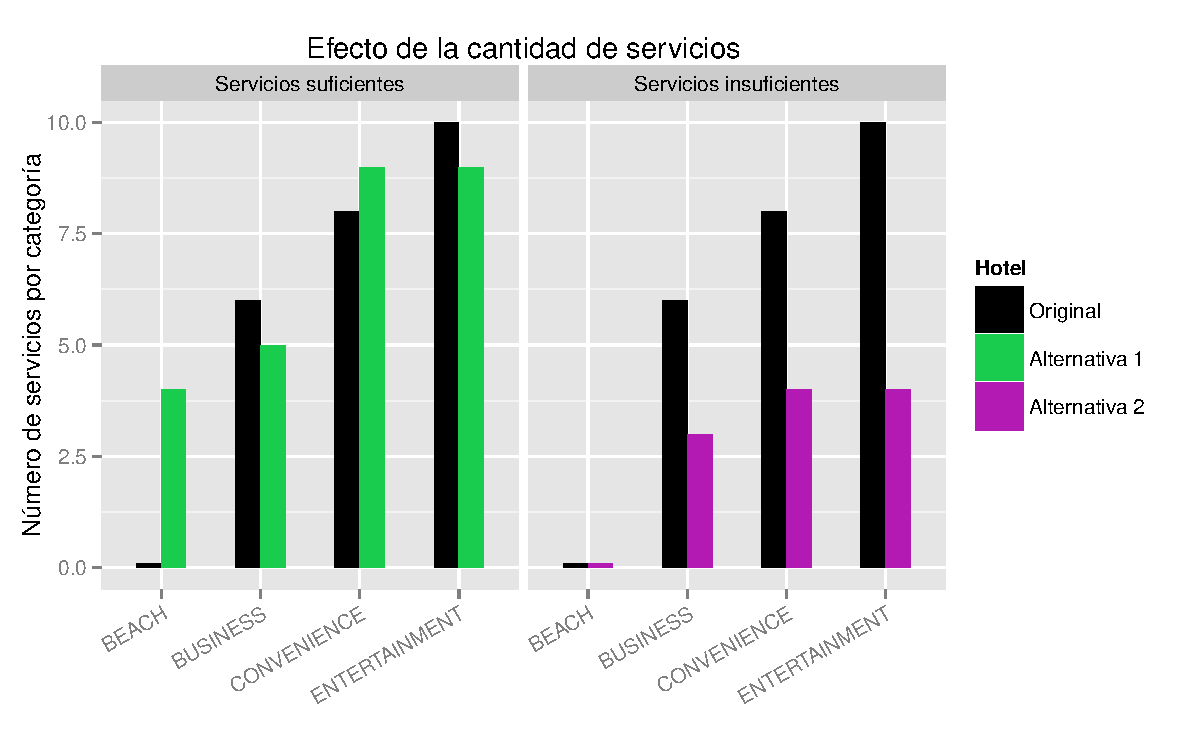
\includegraphics[width=\textwidth]{imagenes/simserv.pdf}
	\caption{\label{simserv} Ejemplos de similitud de servicios para 4 categorías distintas. El hotel verde se parece al negro porque no le faltan muchos servicios que el negro sí tiene. En contraste, al hotel morado le faltan muchos servicios.}
\end{figure}

Lo que buscaremos entonces es penalizar los servicios que le falten a un hotel a la hora de buscar candidatos. Para ello definimos la siguiente función:
\begin{defn}[Pseudodistancia \emph{hinge}]
Sean $x, y \in \R^n$. Definimos la pseudodistancia \emph{hinge} de $x$ a $y$ como sigue:
\[
d_h(x,y) = \sum_{k=1}^n \max\{x_k - y_k, 0\}
\]
\end{defn}
Esta función de pérdida no cumple la propiedad (\ref{dsim}) porque no es simétrica, como es evidente en la figura (\ref{fig:hingeloss}). Por lo tanto, se trata de una \emph{pseudodistancia}. Esta propiedad de $d_h(\cdot, \cdot)$ es algo positivo en el contexto de nuestro problema porque refleja justamente la asimetría de la relación entre los servicios del hotel buscado y los recomendados. Aplicando esta pseudodistancia a los vectores característicos de dos hoteles $c_i$ y $c_j$ obtenemos:
\shorthandoff{<>}
\begin{figure}
	\centering
	\begin{tikzpicture}[xscale=3.5, yscale = 3.5]
		\draw[->] (-1.2,0) -- (1.2,0);
		\draw[->] (0,-0.5) -- (0,1.2);
		\node at (1,-0.1) {$x - y$};
		\node at (-0.8,0.1) {$\max\{x - y, 0\}$};
		\node at (-0.6,1) {$|x - y|$};
		\draw[ultra thick, domain=-1:1] plot (\x, {max(\x,0)});
		\draw[red, dashed, ultra thick, domain=-1:1] plot (\x, {abs(\x)});
	\end{tikzpicture}
	\caption{Ejemplo univariado. Distancia entre $x$ y $y$ usando valor absoluto (- - -) y pérdida \emph{hinge} (---). La pérdida \emph{hinge} no penaliza el caso en que $y > x$. \label{fig:hingeloss}}
\end{figure}
\shorthandon{<>}
\[
d_h(c_i, c_j) = \sum_{k=1}^{n_c} \max\{c_{ki} - c_{kj}, 0\}
\]
La lógica detrás de esta cantidad es la siguiente: la resta $c_{ki} - c_{kj}$ representa la diferencia en número de servicios que el hotel $i$ tiene sobre el $j$ en la categoría $k$. Dado nuestro supuesto de que los servicios son perfectamente intercambiables, tenemos que $c_{ki} \geq c_{kj}$ si y sólo si el hotel $i$ es ``mejor'' que el $j$ en la categoría k, y por lo tanto $j$ incurrirá en una penalización de ese número por su falta de servicios. En el caso en que $i$ sea peor que $j$, es decir, cuando $c_{ki} \leq c_{kj}$, no se penaliza a $j$ y el máximo hace que se sume 0 a la distancia. En conclusión, $d_h(c_i, c_j) =$ \emph{cantidad de servicios que $j$ no tiene pero $i$ sí, tomando en cuenta los servicios en cada categoría como sustitutos perfectos}.

Para etapas posteriores, cabe mencionar que dado que el número de servicios y de categorías es finito, hay una cota máxima a la distancia \emph{hinge} entre dos hoteles, digamos $M_h$, que además coincide con el número total de servicios $n_s$ (el caso se da cuando un hotel no tiene servicios y el otro tiene todos los servicios disponibles). Si bien $d_h(\cdot, \cdot)$ tiene una interpretación muy conveniente, cambiarla de escala es más útil para el modelo y hace que sea casi inmediato ver si una distancia es grande o chica, independientemente de la cantidad de servicios en el sistema. Para ello simplemente la dividimos entre $M_h$, de modo que queda entre 0 y 1, lo que también permite definir una similitud asociada:
\begin{defn}[Pseudodistancia \emph{hinge} normalizada y similitud de servicios]
Sean $x, y \in \R^n$. Definimos la pseudodistancia \emph{hinge} normalizada de $x$ a $y$ como sigue:
\[
d_{hn}(x,y) = \frac{1}{n_s}d_h(x,y)
\]
Definimos la similitud de servicios (o basada en \emph{hinge}) entre $x$ e $y$ como sigue:
\[
sim_h(x,y) = 1 - d_{hn}(x,y)
\]
\end{defn}

\subsection*{Similitud de perfil}

Si bien la pseudodistancia \emph{hinge} captura muy bien la falta de servicios de los hoteles candidatos, no es capaz de diferenciar adecuadamente los perfiles de los hoteles. En la gráfica (\ref{simperf}) ilustramos este hecho con dos ejemplos.
\begin{figure}[ht]
	\centering
	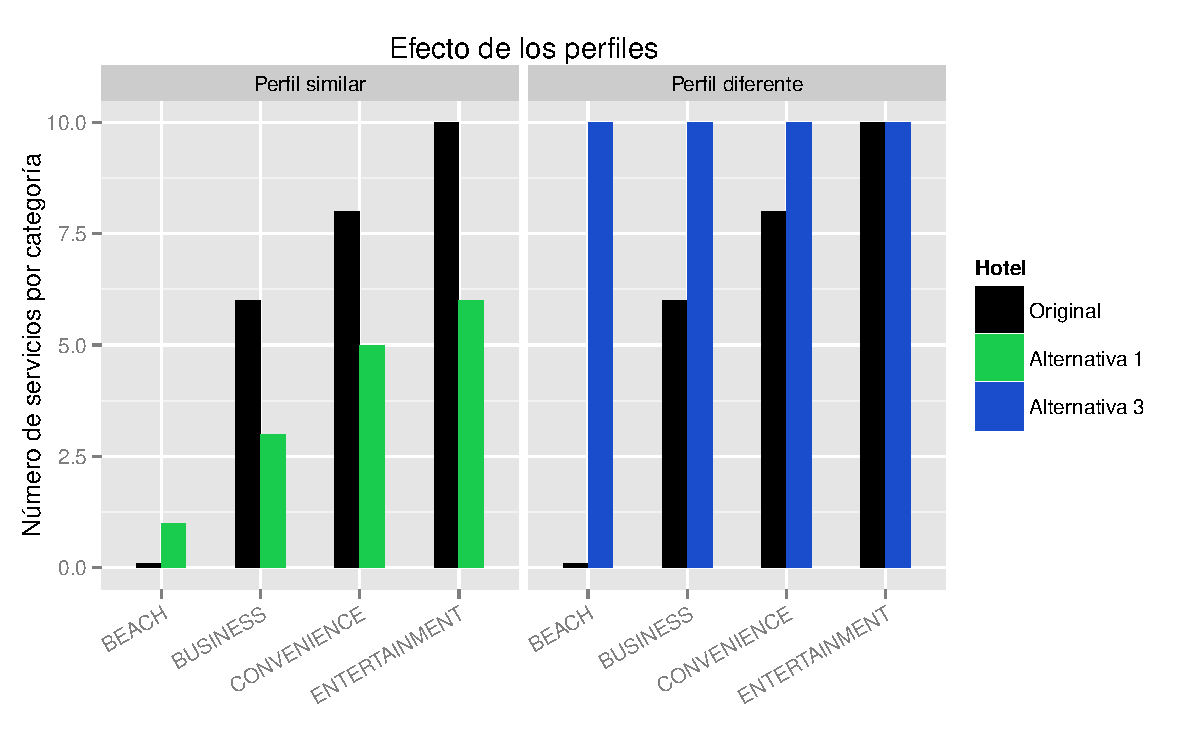
\includegraphics[width=\textwidth]{imagenes/simperf.pdf}
	\caption{\label{simperf} Ejemplos de similitud de perfil para 4 categorías distintas. El hotel verde se parece al negro porque aunque le faltan servicios, tiene aproximadamente la misma proporción de sus servicios en cada categoría. El hotel azul tiene muchos servicios, pero tiene un enfoque distinto (en este caso es un hotel de súper lujo muy enfocado a playa, mientras que el negro no tiene playa).}
\end{figure}

Una manera de modelar el perfil de un hotel es interpretando el número de servicios en cada categoría no como un número absoluto, sino como una \emph{proporción} de los servicios disponibles. Es decir, tener $m$ servicios en la categoría $k$ es mucho o poco dependiendo del número total de servicios que tiene el hotel. Como en este caso cualquier diferencia de perfil afecta, necesitamos una distancia simétrica, que definimos a continuación.
\begin{defn}[Divergencia y similitud de perfil]
Sean $x, y \in \R$. Definimos la divergencia entre $x$ e $y$ como sigue:
\[
d_{div}(x, y) = \frac{1}{2}\sum_{k=1}^n \left|\frac{x_i}{\sum_j x_j} - \frac{y_i}{\sum_j y_j}\right|,
\]
es decir, la distancia absoluta entre los vectores normalizados por su suma. Definimos también la similitud de perfil (o basada en la divergencia) como
\[
sim_{div}(x,y) = 1 - d_{div}(x,y)
\]
\end{defn}
Usando el hecho de que $d(x,y) = \sum_{k=1}^n | x_i - y_i |$ es una distancia, es fácil ver que la divergencia cumple las propiedades (\ref{dpos}), (\ref{dsim}) y (\ref{dtri}). La única propiedad que no tiene es la (\ref{dmin}), puesto que $d_{div}(x,y) = d_{div}(x,\lambda y)$ para cualquier $\lambda > 0$. Sin embargo, en el contexto de la comparación de hoteles este hecho es poco relevante y, para todo fin práctico, la divergencia tendrá las propiedades que necesitamos en una distancia. Además de ello, tiene la ventaja de que quita la escala primero y luego compara los vectores en un espacio equitativo. Regresando a la gráfica (\ref{simperf}), notamos que bajo este criterio, el hotel verde es prácticamente idéntico al negro, incluso a pesar de que es un hotel de mucho menor nivel, debido a que ambos tienen una distribución similar de servicios en cada una de las categorías. Por otra parte, aunque el azul tiene más servicios en cada categoría, tiene una distribución más uniforme que el negro y, por lo tanto, su distancia basada en divergencia será grande.

Finalmente, es importante mencionar que, dado que los vectores normalizados suman 1 y los estamos restando, la divergencia nunca puede pasar de 1 (nótese el factor 1/2 en la definición). Por lo tanto, la similitud que definimos, $sim_{div}(\cdot,\cdot)$, en efecto tiene sentido. La falla de la divergencia por cumplir (\ref{dmin}) resultará únicamente en que la similitud entre dos hoteles pueda ser máxima aunque los hoteles sean distintos.

\subsection*{Similitud completa}

En las secciones anteriores resolvimos individualmente los tres puntos críticos. Por un lado, al mudar el análisis a la escala de categorías resolvimos el problema del ruido. Por otro, cada uno de los criterios de similitud de servicios y de perfil resuelve uno de los otros dos problemas. Como ninguno de los dos es suficiente por sí solo, los integraremos en una sola medida de similitud que sí tome en cuenta todo. La dificultad radica en cómo hacerlo sin perder información y dándole un peso apropiado a cada uno de los componentes.

De este punto en adelante trabajaremos nuevamente con similitudes, porque es más cómodo hablar de similitudes y porque además son equivalentes a sus distancias asociadas. Dado que tanto la similitud de servicios como la de perfil están en escalas equiparables, una manera razonable de combinarlas sería promediarlas. Sin embargo, podrían tener diferentes niveles de variabilidad, por lo que es prudente permitir la posibilidad de utilizar una ponderación distinta de $1/2$.
\begin{defn}[Similitud entre hoteles]
Sea $\alpha \in (0,1)$ y sean $i, j$ hoteles en $\HH$. Definimos la similitud con parámetro $\alpha$ entre $i$ y $j$ como sigue:
\[
sim_\alpha(c_i, c_j) = \alpha sim_h(c_i, c_j) + (1 - \alpha) sim_{div}(c_i, c_j)
\]
\end{defn}
Cabe mencionar que la similitud entre hoteles no es simétrica porque está basada en parte en la similitud de servicios. Es decir, no necesariamente se cumple que $sim_\alpha(c_i, c_j) = sim_\alpha(c_j, c_i)$.

Ya habiendo establecido la forma de combinar las dos medidas de similitud, el siguiente paso es elegir un valor apropiado de $\alpha$, que de preferencia sea óptima con respecto a algún criterio. Para ello, hay que notar que aunque ambas similitudes están entre 0 y 1, podrían tener niveles de variación y medias distintos, por lo que utilizar $\alpha = 1/2$ podría no ser una buena idea.
\begin{figure}[ht]
	\centering
	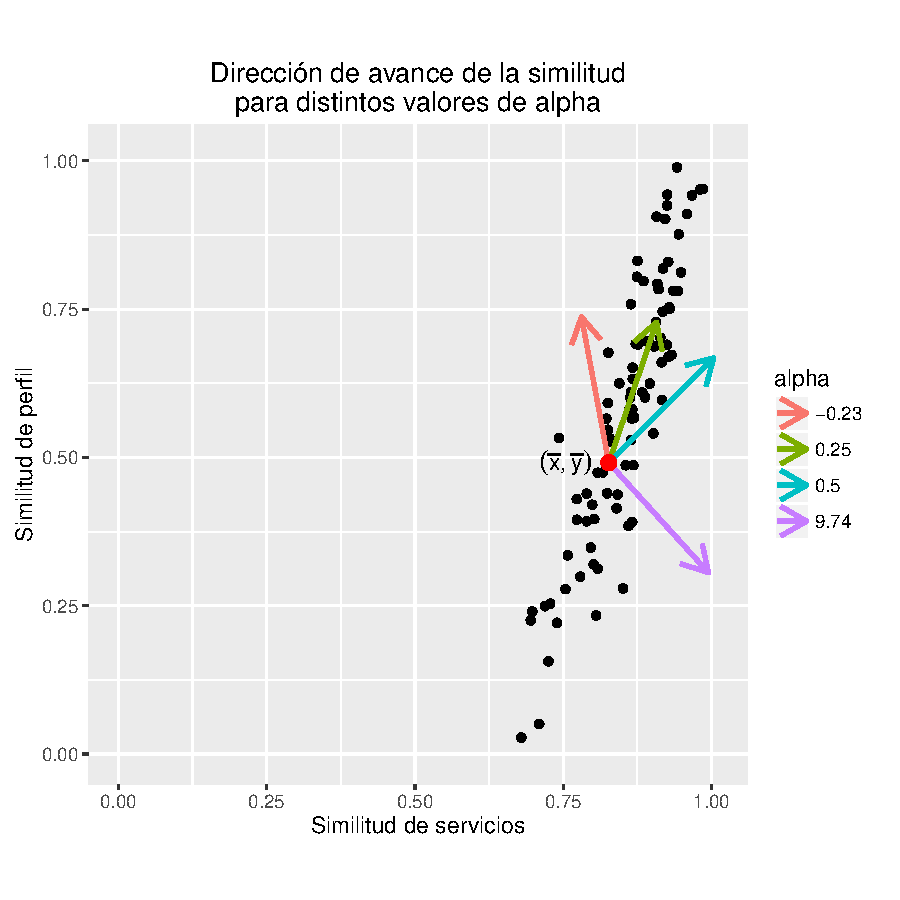
\includegraphics[width=0.8\textwidth]{imagenes/alpha.pdf}
	\caption{\label{alpha} La elección de $\alpha$ determina la dirección en la que avanza la similitud total al variar la de servicios y la de perfil.}
\end{figure}

En la figura (\ref{alpha}) ilustramos las direcciones de avance del \emph{score} al variar $\alpha$. Es claro ver que conviene utilizar un valor de $\alpha$ entre 0 y 1, como pedimos en la definición, porque de otro modo alguna de las medidas contribuirá negativamente al \emph{score}, como lo ilustran las flechas rosa y violeta. La turquesa muestra la dirección en la que crecería el \emph{score} si utilizáramos $\alpha = 1/2$. Como en este ejemplo la similitud de servicios tiene una menor variabilidad que la de perfil, si escogiéramos ese valor, le estaríamos dando un mayor peso al perfil. Si quisiéramos darles igual peso a ambas medidas, deberíamos utilizar $\alpha = 1/4$, como ilustra la flecha verde.

Dado que queremos identificar hoteles similares, un buen criterio para decidir el valor de $\alpha$ es de manera que maximice el poder discriminatorio del \emph{score}. Es decir, que capture en un solo número la mayor cantidad posible de la información contenida en las dos medidas de similitud. En términos estadísticos, lo que queremos es obtener $\alpha \in (0,1)$ tal que se maximice la varianza del \emph{score} resultante. El método conocido como Análisis de Componentes Principales (ACP), que se puede encontrar en muchos libros de texto, como por ejemplo en \cite{elements}, hace algo muy similar a eso, con la pequeña diferencia de que no obtiene $\alpha$ entre 0 y 1. Sin embargo, dado que lo que importa es la dirección de la flecha generada por $\alpha$, podremos solucionar este inconveniente con una simple transformación.

Como queremos calcular el valor óptimo de $\alpha$ para las recomendaciones que haremos, tenemos que hacer el análisis con todas (o una muestra suficiente de) las recomendaciones de todos los hoteles. La forma de hacerlo es como sigue:
\begin{enumerate}
	\item Establecer los parámetros de los filtros estáticos de precio y distancia.
	\item Para cada hotel $i$, generamos $\HH_i^2$ como está descrito en R\ref{r:distanciaestatica}.
	\item Para todo $j \in \HH_i^2$, calculamos
	\begin{align*}
		h_{ij} &:= sim_h(c_i, c_j)\\
		d_{ij} &:= sim_{div}(c_i, c_j)
	\end{align*}
	\item Insertamos cada pareja $(h_{ij}, d_{ij})$ como un renglón en una matriz $A$, con dos columnas y número de renglones igual a $\sum_i |\HH_i^2|$. Es decir, los renglones de $A$ pueden ser representados como en la figura (\ref{alpha}).
	\item Corremos ACP sobre $A$ y obtenemos el vector propio asociado a la primera componente principal, digamos
	\[
	\vec{a} = (a_h, a_d)
	\]
	$\vec{a}$ son las ponderaciones correspondientes a los servicios y al perfil, respectivamente, que maximizan la varianza del \emph{score} resultante,
	\[
	sim_{\vec{a}}(c_i, c_j) = a_h sim_h(c_i, c_j) + a_d sim_{div}(c_i, c_j)
	\]
	\item Como vimos, el vector $\vec{a}$ define la dirección que buscamos, pero sus componentes no necesariamente suman 1. Para forzar a que esto suceda, si $a_h, a_d \geq 0$, basta dividir $\vec{a}$ entre $a_h + a_d$ para obtener lo que deseamos, puesto que $\vec{a} / (a_h + a_d)$ apuntará en la misma dirección que $\vec{a}$. Si este es el caso, podemos definir
	\begin{align*}
		\alpha^* &:= \frac{a_h}{a_h + a_d}\\
		1 - \alpha^* &:= \frac{a_d}{a_h + a_d}
	\end{align*}
	Es fácil ver que la similitud resultante es equivalente a la del punto anterior, notando que
	\begin{align*}
	sim_{\alpha^*}(c_i, c_j) &= \alpha^* sim_h(c_i, c_j) + (1 - \alpha^*) sim_{div}(c_i, c_j)\\
	&= \frac{a_h}{a_h + a_d} sim_h(c_i, c_j) + \frac{a_d}{a_h + a_d} sim_{div}(c_i, c_j)\\
	&= \frac{1}{a_h + a_d} (a_h sim_h(c_i, c_j) + a_d sim_{div}(c_i, c_j))\\
	&= \frac{1}{a_h + a_d} sim_{\vec{a}}(c_i, c_j)
	\end{align*}
\end{enumerate}
De este punto en adelante únicamente utilizaremos la similitud completa utilizando $\alpha^*$. La siguiente definición nos ayudará a facilitar la exposición.
\begin{defn}[Score]
La similitud completa que resulta de utilizar $\alpha^*$ se denomina \emph{score}, es decir:
\[
score(i,j) := sim_{\alpha^*}(c_i, c_j)
\]
\end{defn}
El \emph{score} condensa todas las propiedades que buscábamos en una medida de similitud y que no tenga los tres problemas expuestos al principio de esta sección. Claramente no presentará la volatilidad de las medidas basadas en servicios crudos porque está basada en categorías. Sin embargo, este mismo hecho genera potencial de enmascaramiento si las categorías no están bien elegidas. Esto se debe a que si son heterogéneas y no consisten de servicios que sean sustitutos más o menos cercanos, puede haber falsos positivos y falsos negativos al calcular cualquier medida basada en ellos. En cuanto al segundo punto, suponiendo que las categorías en efecto son apropiadas, la parte de \emph{hinge} del \emph{score} garantizará hasta cierto punto que no se recomiende hoteles con demasiado pocos de los servicios de interés. Finalmente, el hecho de que haya una colaboración de la similitud basada en la divergencia evita que se recomiende hoteles con un perfil muy distinto al original.

Suponiendo que el \emph{score} es una medida satisfactoria de similitud, podemos proseguir a los siguientes componentes del sistema de recomendación, que tomarán en cuenta aspectos físicos y temporales que son imposibles de capturar utilizando únicamente información de los servicios de los hoteles.

\section{Distancia: filtro dinámico}

El concepto de ``hotel similar'' que buscamos en este caso tiene que ver no sólo con que los hoteles sean en sí mismos similares, sino que además estén cerca. La dificultad es que la noción de lo que significa la palabra ``cerca'' varía de lugar a lugar. Por ejemplo, en una zona con una alta densidad de hoteles, como Reforma Centro en la Ciudad de México, un hotel es considerado cercano si está a, digamos, no más de 1 ó 2 kilómetros. Una opción en el Aeropuerto Benito Juárez no es aceptable y difícilmente alguien diría que dicha opción está cerca de Reforma Centro (aunque en realidad está a 15 km). Sin embargo, en una zona despoblada como la Riviera Maya, en la que todo el transporte es por carretera, 15 kilómetros son 10 minutos en coche, y de hecho hay muchos hoteles que no tienen vecinos a menos de varios kilómetros de distancia. La moraleja es que la distancia se percibe distinto según la zona, por lo que debemos utilizar algún criterio adaptativo.

Una primera idea para incorporar la distancia en el modelo fue meterla de alguna manera en el \emph{score}, por ejemplo, como un tercer término en el promedio. Sin embargo, encontramos un argumento que sugiere que esto podría no ser la mejor idea: Supongamos que buscamos recomendaciones para el hotel A y tenemos dos candidatos, B y C. Dada la densidad de la zona, ambos están ``cerca'' de A, pero resulta que B está a la mitad de distancia de A que C. Además, supongamos que C se parece un poco más a A que B. La pregunta es entonces: ¿deberíamos recomendar a B sobre C aunque se parece menos y dado que ambos están cerca? Creemos que la respuesta a este ejercicio es claramente que no, que si ambos están cerca, es preferible el hotel más similar. Esta manera de pensar nos llevó a la conclusión de que incorporar la distancia de manera suave (como por ejemplo dándole una ponderación en el \emph{score}) tal vez no sea la mejor alternativa. Por ello decidimos mejor incorporarla en la forma de un filtro dinámico. Para ello hay que seguir dos pasos:
\begin{enumerate}
	\item Definir qué entendemos por hoteles cercanos.
	\item Pasar a la siguiente ronda del modelo los hoteles que cumplen dicho criterio, ordenados por \emph{score}, es decir, por qué tan parecidos son al hotel en cuestión.
\end{enumerate}
El paso crítico para este método es la definición de cercanía. Una forma de hacerlo es elegir, por ejemplo, los 20 ó 30 hoteles más cercanos al hotel en cuestión. Sin embargo, este enfoque ingenuo tiene un problema grave: si un hotel es único en su categoría en la zona (por ejemplo es de 5 estrellas en un pueblo pequeño), entonces posiblemente los 20 hoteles más cercanos a él no se parezcan en lo absoluto. En estos casos debería permitirse una mayor flexibilidad de búsqueda en favor de obtener mejores recomendaciones. Para lograr esto, le damos un peso distinto a los hoteles cercanos, según su similitud al hotel original, es decir, acumulamos \emph{score} en lugar de cantidad. De este modo, en zonas con muchos hoteles apropiados, la acumulación de \emph{score} será rápida y por lo tanto el radio de búsqueda será pequeño. En contraste, si no hay muchos hoteles similares, el \emph{score} se acumulará más lentamente y por consiguiente el radio será mayor. En la figura (\ref{fig:distdin}) ilustramos lo que sucede y en la siguiente definición describimos el proceso formalmente.
\begin{figure}[ht]
	\centering
	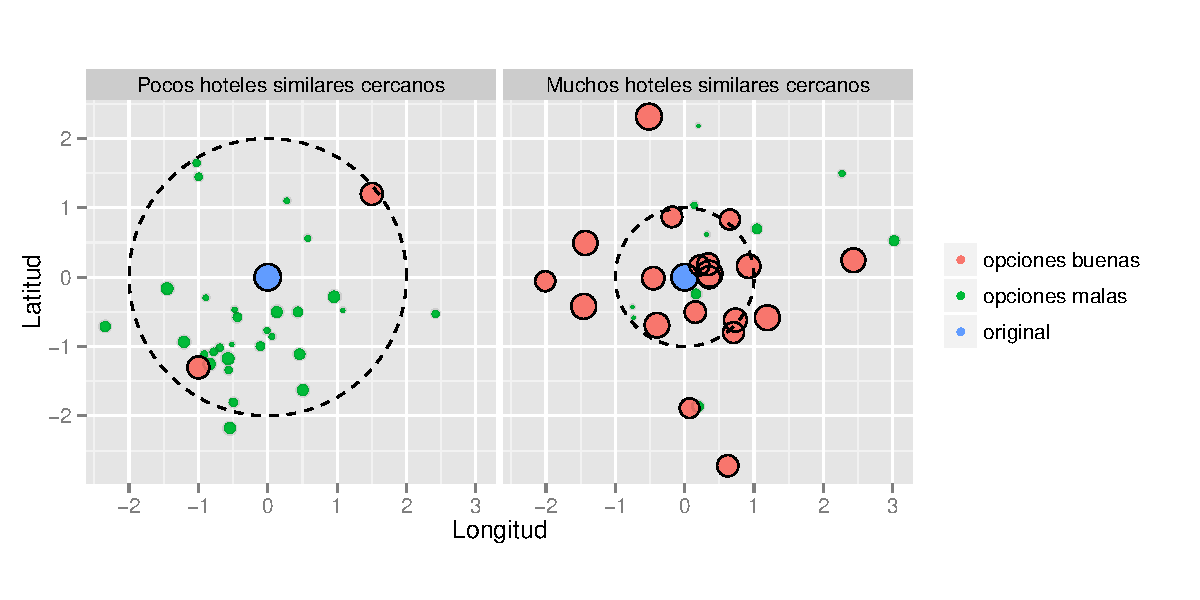
\includegraphics[width=\textwidth]{imagenes/distdin.pdf}
	\caption{\label{fig:distdin} El filtro debe ser más laxo cuando hay pocos hoteles similares cercanos (izquierda) y más estricto cuando hay más (derecha).}
\end{figure}
\begin{regla}[Distancia: filtro dinámico] \label{r:distanciadinamica}
La función de acumulación de score al alejarse del hotel $i$, $F_i: \R \to \R$, está definida para cada $d \in \R$ como sigue:
\[
F_i(d) = \sum_{j | d_{geo}(i,j) < d} score(i,j)
\]
Para una cantidad predefinida a acumular, digamos $w_{inner} > 0$, definimos la \textbf{cerca interior} como el círculo centrado en el hotel $i$ y con radio dado por
\[
r_{inner} = \arg\min_d \{F_i(d) \geq w_{inner}\},
\]
es decir, la mínima distancia que garantice que se acumula al menos $w_{inner}$ de \emph{score} dentro de la cerca interior. Los hoteles que pasan a la siguiente ronda son entonces los que estén en la cerca interior:
\[
\HH_i^3 = \{j \in \HH_i^2 : d_{geo}(i,j) \leq r_{inner}\}
\]
\end{regla}
La regla anterior es fácil de entender a la luz de la intuición de lo que queremos lograr. Si un hotel es único en su área, los hoteles cercanos no se parecerán a él, lo que provocará que $F_i$ crezca lentamente y, por consiguiente, que $r_{inner}$ sea grande. Por el contrario, si hay muchos hoteles parecidos a $i$ cerca, entonces $F_i$ crecerá rápidamente y por lo tanto $r_{inner}$ será más pequeño.

\section{Precios dinámicos}

Un punto que hasta el momento no hemos tratado son las posibles promociones que los hoteles puedan ofrecer. Si bien el objetivo principal de este sistema es recomendar hoteles similares y no necesariamente descuentos, es deseable que éstos tuvieran algún impacto. Para ello notemos que el filtro estático de precio toma en cuenta el promedio de los precios en el largo plazo. Eso quiere decir que si un hotel baja sus precios temporalmente, podría ser un candidato para otros hoteles más baratos, pero tanto la baja de los precios como su impacto se ven diluidos en el promedio. Una forma de suavizar este problema es filtrar con los precios en la fecha de la búsqueda en lugar de los promedios. Es decir que, si bien debemos calcular $\alpha$ y $r_{inner}$ con $\HH_i^2$ tal como lo hemos descrito hasta el momento, conviene utilizar
\begin{align}
	\mathcal{D^*} = \text{ período para el cual se busca reservar}
\end{align}
para calcular los precios en lugar del período histórico largo $\mathcal{D}$.
\begin{regla}[Precio dinámico] \label{r:preciodinamico}
Dadas $\alpha$ y $r_{inner}$ obtenidas en R\ref{r:preciolargo}, R\ref{r:distanciaestatica} y R\ref{r:distanciadinamica}, denotamos las \textbf{recomendaciones finales} por
\[
\RR_i = \{j \in \HH : p^{D^*}_j \leq (1 + \gamma)p^{D^*}_i \text{,  } d_{geo}(i,j) \leq r_{inner}\},
\]
y los hoteles se presentarán ordenados por \emph{score}, de mayor a menor.
\end{regla}
Hay que tener en cuenta que este último cambio aumenta considerablemente el costo computacional de calcular las recomendaciones, ya que habrá que conseguir los precios de todos los hoteles cercanos a $i$ en las fechas apropiadas cada vez que un usuario entre a la página del hotel (sería inviable almacenar todas las recomendaciones para todas las fechas posibles). Compárese esto con utilizar precios estáticos de largo plazo, en cuyo caso se puede almacenar las recomendaciones del hotel $i$ una sola vez, dado que serán las mismas para todos los usuarios.

Si se considera que la carga computacional es demasiado pesada para la infraestructura en la que se correrá el sistema de recomendación, se puede omitir los precios dinámicos, poniendo $\RR := \HH_i^3$ y mostrando los hoteles ordenados por \emph{score} de la misma manera que en R\ref{r:preciodinamico}.

\section{Consideraciones prácticas}

Un último tema que hay que abordar es la posibilidad de que algún hotel no posea suficientes alternativas para generar las recomendaciones. Esto podría darse por dos razones, a saber, (1) debido a que la zona en donde se encuentra el hotel es de baja densidad y por lo tanto no hay suficientes hoteles en su cerca exterior, o (2) porque el hotel es atípicamente barato en comparación con sus vecinos, en cuyo caso el filtro de precio le impedirá ver muchos de los hoteles vecinos. En ambos casos, un asesor deberá utilizar su \emph{ingenio} para salir de paso. Lo que es indispensable es que \emph{siempre} recomiende algo, aunque sea lo menos peor cuando no tenga alternativa.

Para aliviar el primer problema el procedimiento es simple: como no queremos que se queden vacías las recomendaciones, ignoramos todo lo anterior y regresamos un número pequeño predefinido de hoteles lo más cercanos que se pueda, ordenados por distancia. Decidimos ignorar el \emph{score} en estos casos porque, dado que hay muy pocas opciones, creemos que hay que darle prioridad al destino en particular que buscó el cliente. Si, por otro lado, sí hay suficientes hoteles dentro de la cerca exterior, pero el filtro de precio es demasiado estricto, entonces ignoramos por completo este filtro.
\begin{regla}[Casos extremos] \label{r:casosextremos}
Sea $rec_{min} > 0$ el mínimo número de recomendaciones que se desea.
\begin{enumerate}[(I)]
	\item Si $|\HH_i^2| < rec_{min}$, entonces redefinimos
		\[
			\HH_i^1 = \HH
		\]
	\item Si aún después del paso anterior $|\HH_i^2| < rec_{min}$, entonces ignoramos todas las reglas y recomendamos los hoteles en
	\[
		\RR_i^{ex} = \{j \in \HH : j \text{ es uno de los } rec_{min} \text{ hoteles más cercanos a } i\}
	\]
	Además, ignoramos el score y los presentamos ordenados por distancia al hotel $i$.
	\item Las dos reglas anteriores aplican de manera análoga para $\HH_i^{1*}$ y $\HH_i^{2*}$, los equivalentes a $\HH_i^{1}$ y $\HH_i^{2}$ que utilizan el precio dinámico.
\end{enumerate}
\end{regla}

\section{Resumen del proceso}

El procedimiento descrito anteriormente es largo y puede ser difícil de asimilar en su conjunto, de modo que presentamos aquí una versión resumida:
\begin{enumerate}
	\item Sean $i$ un hotel, $D$ un periodo largo y $D^*$ el periodo en el que se desea reservar.
	\item Calculamos $\alpha$ y $r_{inner}$ como está descrito en R\ref{r:preciolargo}, R\ref{r:distanciaestatica} y R\ref{r:distanciadinamica}.
	\item Checamos los casos extremos descritos en R\ref{r:casosextremos}. Si ninguno aplica, continuamos; si resulta el caso (II), entonces recalculamos el paso (2) y continuamos al (4); si resulta el caso (I), recomendamos con $\RR_i^{ex}$ por distancia y terminamos.
	\item Generamos las recomendaciones finales como está descrito en R\ref{r:preciodinamico} y las presentamos ordenadas por \emph{score}.
\end{enumerate}

\section{Comentarios}

Antes de terminar el capítulo, hay un punto que nos gustaría resaltar y es por qué no decidimos simplemente basar la distancia en la norma 1. La respuesta corta es que es muy exigente. Aunado a ello, no nos permite ponderar fácilmente las contribuciones del perfil y de los servicios. Es posible que haya alguna manera de alterar esta distancia para capturar la asimetría de la disponibilidad de servicios. De ninguna forma afirmamos que no haya alternativas al menos tan buenas como la nuestra, pero dado que obtuvimos resultados satisfactorios, nos quedamos con el método presentado anteriormente. Investigar nuevas medidas de distancia sería un buen tema de trabajo futuro.




% ----------------------------------------------------------------------------------------------------
\chapter{Implementación} \label{cap:3}

En este capítulo describiremos algunos detalles adicionales al modelo matemático que son necesarios para la implementación del sistema de recomendación en el mundo real. Hablaremos de qué fuentes obtendremos los datos necesarios para el modelo y de qué haremos en los casos en los que la calidad de los mismos no sea la necesaria para correr el modelo.

\section{Información}

En esta sección describiremos el qué, el cómo y el dónde de la información que utilizamos para el sistema de recomendación. Para ello hay que notar que necesita dos insumos para funcionar. El primero es información a nivel hotel, como son los nombres, los detalles geográficos y los precios. El segundo consiste de la información de los servicios del hotel. En los siguientes dos apartados describiremos cada uno con mayor detalle.

\subsection*{Información de hoteles}

La tabla de información de hoteles debe tener por lo menos las siguientes columnas para que el modelo funcione:
\begin{itemize}
	\item Clave del hotel.
	\item Latitud y longitud.
	\item Precio promedio por noche en alguna moneda unificada (USD) y en algún período razonablemente largo, digamos uno o dos años.
\end{itemize}
Opcionalmente se puede agregar el volumen de noches y la utilidad bruta en el mismo periodo para hacer algunos análisis, aunque el modelo estrictamente no los necesita.

Para obtener esta tabla es necesario notar que no hay un catálogo de precios, por lo que los tuvimos que estimar mediante las reservaciones que se hicieron en el periodo analizado. Es decir, el precio promedio por noche en el periodo $D$ (en USD) de un hotel dado es:
\[
\text{Precio promedio} = \frac{\text{Suma de importes de las reservas en el periodo } D}{\text{Suma de noches reservadas en el periodo } D}
\]
Para acceder fácilmente esta información generamos un \gls{sp}\footnote{Ver \emph{Stored Procedure} en el glosario.} en \gls{sqlserver}\footnote{\textit{Ver glosario.}} que recibe una fecha de inicio, hace $D = $ de la fecha proporcionada hasta hoy, y finalmente regresa la tabla con la información de los hoteles. Para la primera versión decidimos utilizar un periodo de 2 años, con el fin de tomar en cuenta un número suficiente de datos históricos y así evitar que los hoteles poco vendidos no tuvieran ningún precio.

\subsection*{Información de servicios}

Las matrices $S$ y $C$, que contienen la información de los servicios y las categorías respectivamente, son bastante ralas. Por esta razón es conveniente almacenarlas como relaciones con un renglón por cada elemento distinto de cero de la matriz correspondiente. Como $S$ es binaria, la almacenaremos en una tabla con dos columnas, clave del hotel y clave del servicio, mientras que $C$ requiere tres: clave del hotel, clave de la categoría y número de servicios en la categoría.

Dado que en la base de datos de Best Day ya está la tabla con los servicios en el formato deseado, basta filtrar los hoteles con información incompleta o de zonas que no nos interesen y ya tenemos la primera tabla. Para obtener la segunda fue necesario primero correr el aglomerado en \texttt{R} utilizando la primera tabla y crear a mano la relación entre los servicios y las categorías que elegimos. Posteriormente bastó pegarle a cada servicio su categoría correspondiente y sumarizar la tabla de servicios utilizando la clave del hotel y la clave de la categoría como llaves; los conteos dentro de cada grupo corresponden a los valores $c_{ij}$. Nuevamente, generamos un \gls{sp} de \gls{sqlserver} para poder obtener esta información con una simple llamada a una función en lugar de una consulta completa.

A continuación describiremos un tema sobre los servicios que es importante en el contexto de la recomendación de hoteles similares.

\subsubsection*{Plan de alimentos}

La decisión de exactamente qué características del hotel cuentan como servicios es subjetiva hasta cierto punto. Hay algunos que no se incluyeron por razones administrativas o de alguna otra índole. Entre ellos están los planes de alimentos, es decir, la cantidad de comidas que incluyen los hoteles. El plan de alimentos puede ser muy importante en algunas regiones vacacionales en donde haya hoteles de tipo ``todo incluido'' mezclados con hoteles que sólo incluyen desayuno, o incluso nada. La razón es que los precios de dos hoteles de las mismas estrellas podrían diferir bastante si uno es todo incluido y el otro no. Por ello es importante incorporar esta información de algún modo en el modelo.

Si bien hay diversas formas en que se podría tomar en cuenta el plan de alimentos en el sistema de recomendación, uno que nos pareció razonable, fácil de implementar y que además funciona bien, es generar una categoría de alimentos en la matriz $C$. La idea es que si dos hoteles tienen el mismo plan de alimentos, tendrán más servicios en común y por lo tanto favoreceremos que se recomienden entre sí, mientras que si difieren, se tendrán que parecer mucho para que salgan en las recomendaciones del otro. Cada hotel puede tener muchos contratos con Best Day y puede vender cuartos con y sin todo incluido, pero en general, es razonable pensar que si un hotel tiene la opción de todo incluido, es parte de la filosofía del hotel. Por ello, para cada hotel elegimos el plan de alimentos que más comidas incluidas tuviera. El resultado es que podemos agregar hasta cuatro servicios por hotel, uno si incluye desayuno, uno si comida, uno si cena y otro si incluye las bebidas. En la matriz $C$ esto se refleja en una nueva categoría que puede tomar cualquier valor entre cero y cuatro.

\section{Sistema de respaldo}

Uno de los grandes temas que surgen en cualquier modelo matemático que esté basado en datos es la calidad de la información. El modelo descrito en el capítulo anterior presupone no sólo que se tiene la información ya en el formato adecuado, sino que además está limpia. La norma en el mundo real es que esto no es así, por lo que será necesario agregar componentes al sistema de recomendación para que funcione incluso cuando la información no sea perfecta. A continuación enlistaremos algunos de los principales problemas que pueden aparecer en este contexto y las posibles soluciones que les podemos dar:
\begin{itemize}
	\item[P1:] El hotel no tiene ninguna reservación en el periodo analizado para obtener los precios.
	\item[S1:] Utilizamos el modelo pero ignoramos los precios por completo.
	\item[P2:] El hotel tiene mal la información de servicios.
	\item[S2:] Tendremos que utilizar un sistema de recomendación alternativo, como por ejemplo el antiguo.
	\item[P3:] El hotel no tiene coordenadas o las coordenadas son incorrectas.
	\item[S3:] No hay nada que podamos hacer salvo conseguirlas de alguna fuente.
\end{itemize}
La primera dificultad no es tan grave porque podemos utilizar el modelo sin problemas, sólo que ignorando los precios. En realidad es lo mejor que podemos hacer y dado que de cualquier forma tiene que ser un hotel muy poco popular, no importa mucho que las recomendaciones no sean óptimas en estos casos.

Los otros dos puntos son más complicados de resolver porque implican que de plano no podemos utilizar el sistema de recomendación. Una forma de mitigar esto es utilizar el sistema de recomendación antiguo de Best Day que está descrito en el capítulo \ref{cap:1}, es decir, tomar los hoteles en el mismo destino y de las mismas estrellas y recomendarlos en el \emph{Sort Order} del momento. La ventaja de esto es que únicamente requiere el destino y las estrellas del hotel para funcionar, por lo que en la mayoría de los casos podremos evitar no recomendar nada.

Si también falla el sistema de recomendación antiguo no hay mucho que podamos hacer, pues o bien ni siquiera tenemos el destino o estrellas del hotel, o no hay ninguna alternativa en el mismo destino. Si detectamos una zona o algún hotel con esta clase de problemas, lo único podríamos hacer es detectar la información faltante o de mala calidad y completarla o limpiarla a mano, según lo requiera el caso.


\section{Otras consideraciones}

Hay algunas otros detalles técnicos que no entran naturalmente en ningún otro lado, pero que sí son importantes. En esta sección los describiremos brevemente con el fin de aclarar por completo la forma en que se debe implementar este sistema de recomendación:
\begin{itemize}
	\item \emph{Software:} Como hemos comentado, el acceso a la base de datos, tanto para el análisis como para producción, se realizó a través del lenguaje \gls{sql}\footnote{Ver glosario.}. En particular, utilizamos procedimientos almacenados de \gls{sqlserver} 2008\footnote{Ver glosario y \cite{sql}.}, optimizados con índices para disminuir el tiempo de ejecución lo más posible. Toda la analítica se llevó a cabo en \gls{r}\footnote{Ver glosario y \cite{R}}, desde el aglomerado jerárquico hasta la generación de las recomendaciones. En el diagrama (\ref{fig:flujo}) de la siguiente sección será más evidente qué partes del sistema se hicieron en qué lenguaje.
	\item \emph{Almacenamiento de las recomendaciones:} En la práctica no es conveniente calcular los conjuntos $\RR_i$ al vuelo por su elevado costo computacional. Por ello los precalculamos para cada hotel y los metimos en una tabla $R$ con tuplas de la forma (hotel buscado, hotel recomendado, \emph{score}). Si se quiere utilizar los precios estáticos, se puede tomar, digamos, los 20 hoteles recomendados con mayor score para cada hotel buscado. Esto disminuye aún bastante el tamaño de $R$ y, por lo tanto, el costo de consultar las recomendaciones de un hotel. Si, por otro lado, se utilizan los precios estáticos, se debe almacenar todos los hoteles en la cerca interior y filtrarlos dinámicamente con los precios de la fecha consultada.
	\item \emph{Actualización de las recomendaciones:} Dado que los hoteles son entidades más o menos estáticas, no tiene mucho sentido actualizarlas demasiado seguido. Basta correr el algoritmo que genera las recomendaciones una vez al mes, cuando mucho, para ir capturando los pequeños cambios que puedan haber ocurrido.
\end{itemize}


\section{Arquitectura final del sistema} \label{sec:arqui}

En la figura (\ref{fig:flujo}) mostramos la arquitectura que el sistema debería tener idealmente. Por un lado, la base de datos analítica alimenta los \glspl{sp} y el aglomerado jerárquico en \gls{r} de los servicios en categorías. Estos procesos se encargan de generar la matriz $C$ y la tabla $H$ con la información de los hoteles, completa con coordenadas y precios. El algoritmo de recomendación corre completamente en \gls{r} y genera una tabla con las recomendaciones. En términos concretos, las entradas y salidas de cada componente son:
\begin{itemize}
	\item \textbf{\texttt{R}: Aglomerado de servicios}
	\begin{itemize}
		\item Entrada: Matriz rala binaria de servicios - hoteles.
		\item Salida: Dendrograma de apoyo para agrupar los servicios manualmente.
	\end{itemize}
	\item \textbf{SP Categorías (\texttt{ObtenerHotelesCategoriasServicios})}
	\begin{itemize}
		\item Entrada: Clave del país (el proceso se efectúa por país), tipo caracter de 2 posiciones.
		\item Salida: Relación de hoteles con sus categorías y número de servicios en cada categoría.
	\end{itemize}
	\item \textbf{SP Hoteles (\texttt{ObtenerDatosHoteles})}
	\begin{itemize}
		\item Entrada: Fecha inicial para el periodo $D$ (la fecha final es el el día actual). Clave del país (el proceso se efectúa por país), tipo caracter de 2 posiciones.
		\item Salida: Tabla de hoteles con coordenadas, precio (USD), utilidades (USD) y número de noches vendidas.
	\end{itemize}
	\item \textbf{\texttt{R}: Algoritmo de recomendación}
	\begin{itemize}
		\item Entrada: Vector de claves de los países para los que se quiere calcular las recomendaciones. Fecha inicial del periodo $D$ (para usar en el SP). Parámetros de control elegidos ($\alpha, r_{outer}, \dots$).
		\item Salida: Tabla (convertida a formato CSV) que tiene la relación hotel - hotel recomendado - prioridad (rango) del hotel recomendado.
	\end{itemize}
\end{itemize}

Ahora bien, la última tabla de salida se debe cargar a la base de datos operativa para entrar a producción. Idealmente, la carga se debería realizar automáticamente, pero dada la baja frecuencia de las actualizaciones, si por alguna razón no es viable hacerlo así, basta con que se pueda hacer manualmente. Una vez que la tabla $R$ está en la base de datos operativa, la página (i.e. nuestro ``vendedor'' electrónico) puede aprovecharla para recomendar de manera más inteligente.



\begin{figure}[ht]
	\centering
	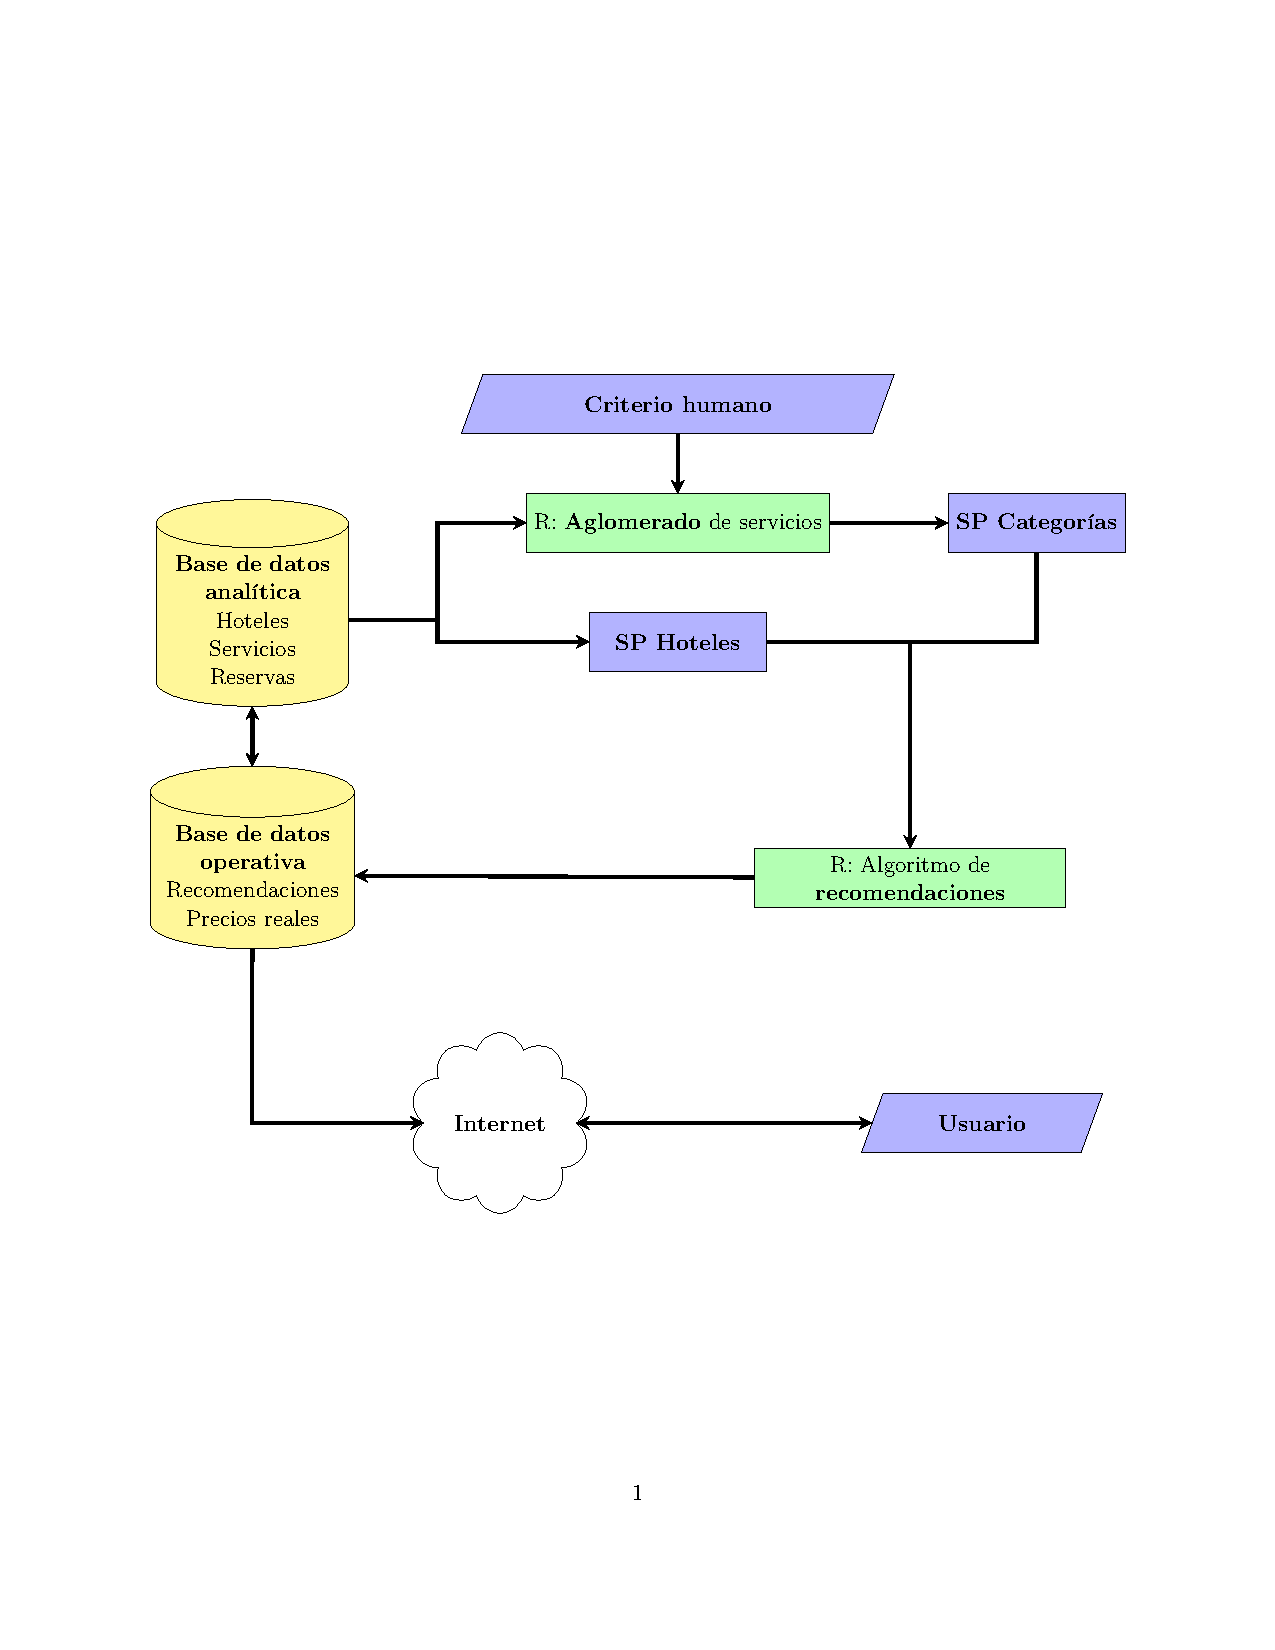
\includegraphics[width=\textwidth]{imagenes/flowchart.pdf}
	\caption{\label{fig:flujo} Diagrama de flujo del sistema de recomendación. Amarillo: bases de datos. Rojo: Interacción humana. Verde: Procesos en \gls{r}. Azul: Procesos en \gls{sql}.}
\end{figure}


% ----------------------------------------------------------------------------------------------------
\chapter{Propiedades teóricas del modelo} \label{cap:4}

Hasta este punto hemos descrito tanto el modelo matemático detrás del sistema de recomendación como las consideraciones prácticas que se debe tener para implementarlo exitosamente. Si bien hemos argumentado todas las decisiones que tomamos en la construcción del sistema, en este capítulo analizaremos algunas de sus propiedades teóricas para ver si en verdad logramos nuestro cometido.

Dado que el sistema que diseñamos consiste en recomendar hoteles partiendo de otros hoteles, resulta natural utilizar la teoría de redes para analizarlo. Las redes son construcciones matemáticas muy versátiles que permiten modelar muchos tipos de fenómenos. En general, cualquier tema de interés que tenga elementos que estén conectados de alguna forma se puede modelar con una red. En este caso, por ejemplo, los elementos serán los hoteles y las conexiones serán las recomendaciones. En las siguientes secciones daremos un brevísimo resumen de algunas de las características principales de las redes y evaluaremos el desempeño del sistema de recomendación utilizando este enfoque.

\section{Teoría básica de redes}

Antes de describir las características de las redes, debemos definir lo que es una red. Una red es esencialmente un conjunto $V$ (que puede incluir cualquier tipo de entidades, individuos, etc.), junto con una colección de conexiones $E$ entre los elementos de $V$. Los elementos en $V$ usualmente se conocen como \emph{nodos} o \emph{vértices}, mientras que las conexiones (en $E$) son llamadas \emph{arcos}. Hay dos principales tipos de redes y sus diferencias radican en si sus arcos son \emph{dirigidos} o \emph{no dirigidos}. Los arcos no dirigidos se utilizan para representar relaciones simétricas, como las conexiones en una red social (como Facebook): ``Juan es amigo de Pedro si y sólo si Pedro es amigo de Juan''. Por otro lado, se utilizan arcos dirigidos cuando las relaciones no necesariamente son bilaterales. Por ejemplo, si se toman los cruces de calles como nodos y los arcos como las calles mismas, cada arco debe tener la dirección de la calle que representa. Cuando se da el caso de relaciones bilaterales en una red dirigida, se puede poner dos arcos, uno en cada dirección. Otras características interesantes de las redes son:
\begin{itemize}
	\item \emph{Variables adicionales de nodos y/o arcos:} Los nodos y los arcos pueden tener otro tipo de características. Por ejemplo, si la red representa una red de tuberías, los arcos podrían tener un flujo máximo asociado.
	\item \emph{Distancia entre nodos:} La distancia entre dos nodos es la mínima cantidad de arcos que se debe atravesar para llegar de uno de los nodos al otro. Si no hay un camino entre dos nodos, decimos que la distancia entre ambos es infinito. Cabe mencionar que si la red es dirigida, sólo está permitido ir en la dirección de los arcos.
	\item \emph{Conectividad:}
	\begin{itemize}
		\item \emph{Fuerte:} Una gráfica es (fuertemente) conexa cuando se puede llegar a cualquier nodo desde cualquier otro nodo, es decir, la distancia entre cualesquiera dos nodos es estrictamente menor que infinito. Nuevamente, en el caso de las gráficas dirigidas sólo se permite transitar en el sentido de los arcos.
		\item \emph{Débil:} Una gráfica dirigida es débilmente conexa si es conexa cuando se ignoran los sentidos de sus arcos.
	\end{itemize}
	\item \emph{Diámetro:} El diámetro de una gráfica conexa (o de un subconjunto conexo de una gráfica) es la distancia máxima entre cualesquiera dos nodos de la gráfica. Como siempre, en las gráficas dirigidas se debe respetar la dirección de los arcos.
	\item \emph{Grados:}
	\begin{itemize}
		\item \emph{Grado de entrada (in-degree):} En redes dirigidas, el número de arcos que le apuntan a un nodo.
		\item \emph{Grado de salida (out-degree):} En redes dirigidas, el número de arcos que salen de un nodo.
		\item \emph{Grado (degree):} En redes dirigidas, corresponde al grado de salida más el grado de entrada. En redes no dirigidas, es el número total de arcos de un nodo.
	\end{itemize}
	\item \emph{PageRank:} Es una medida de importancia que fue diseñada para ver la relevancia de las páginas web. A grandes rasgos, coincide con la probabilidad de que un navegador que da \emph{click} al azar en las ligas (arcos) que ve llegue a una cierta página (nodo). Utilizaremos el PageRank para medir la importancia de los hoteles dentro del sistema, pues representará la probabilidad de que un usuario llegue a un hotel dado si le da \emph{click} a recomendaciones al azar. Al lector interesado lo referimos al artículo original, \cite{pagerank}, y a \cite{mmds} para mayor información sobre el PageRank y sobre redes en general.
\end{itemize}

\section{Modelado del sistema con una red}

Los hoteles y sus recomendaciones se pueden modelar de manera muy natural como una red dirigida tomando los hoteles como nodos y el que un hotel recomiende a otro como los arcos. Con un análisis de redes podremos ver si realmente el sistema recomendación cumple con algunas de las propiedades que buscábamos.

Uno de los primeros problemas que le encontramos al sistema actual es que dentro de una zona y una categoría las recomendaciones son siempre iguales, lo que además de resultar aburrido y poco útil después de poco tiempo, le da un peso excesivo a los hoteles que aparecen hasta arriba de la lista de un destino y ciertas estrellas: todos los clientes que busquen un hotel en ese grupo verán lo mismo. En el mundo de las redes, esto es equivalente a nodos con un grado de entrada muy elevado o con PageRank alto.

Por otro lado, independientemente de lo anterior, las recomendaciones eran cerradas, esto es, no podíamos salir de un cierto grupo de hoteles únicamente por medio de las recomendaciones. Esto equivale a que la red del modelo sea \emph{disconexa} (i.e. no conexa) en lugares en donde no debería. No es problemático que, por ejemplo, la recomendaciones de hoteles en Ciudad Juárez no nos pudieran llevar eventualmente a opciones en Mérida. Sin embargo, sí es poco deseable que eso suceda en secciones geográficamente cercanas. Por ejemplo, si empezamos con un hotel de negocios en Cancún, es deseable que en algunos pocos \emph{clicks} se pueda llegar a uno en la zona hotelera. Ilustramos estos puntos en la gráfica (\ref{fig:disconexo}).
\begin{figure}[h]
	\centering
	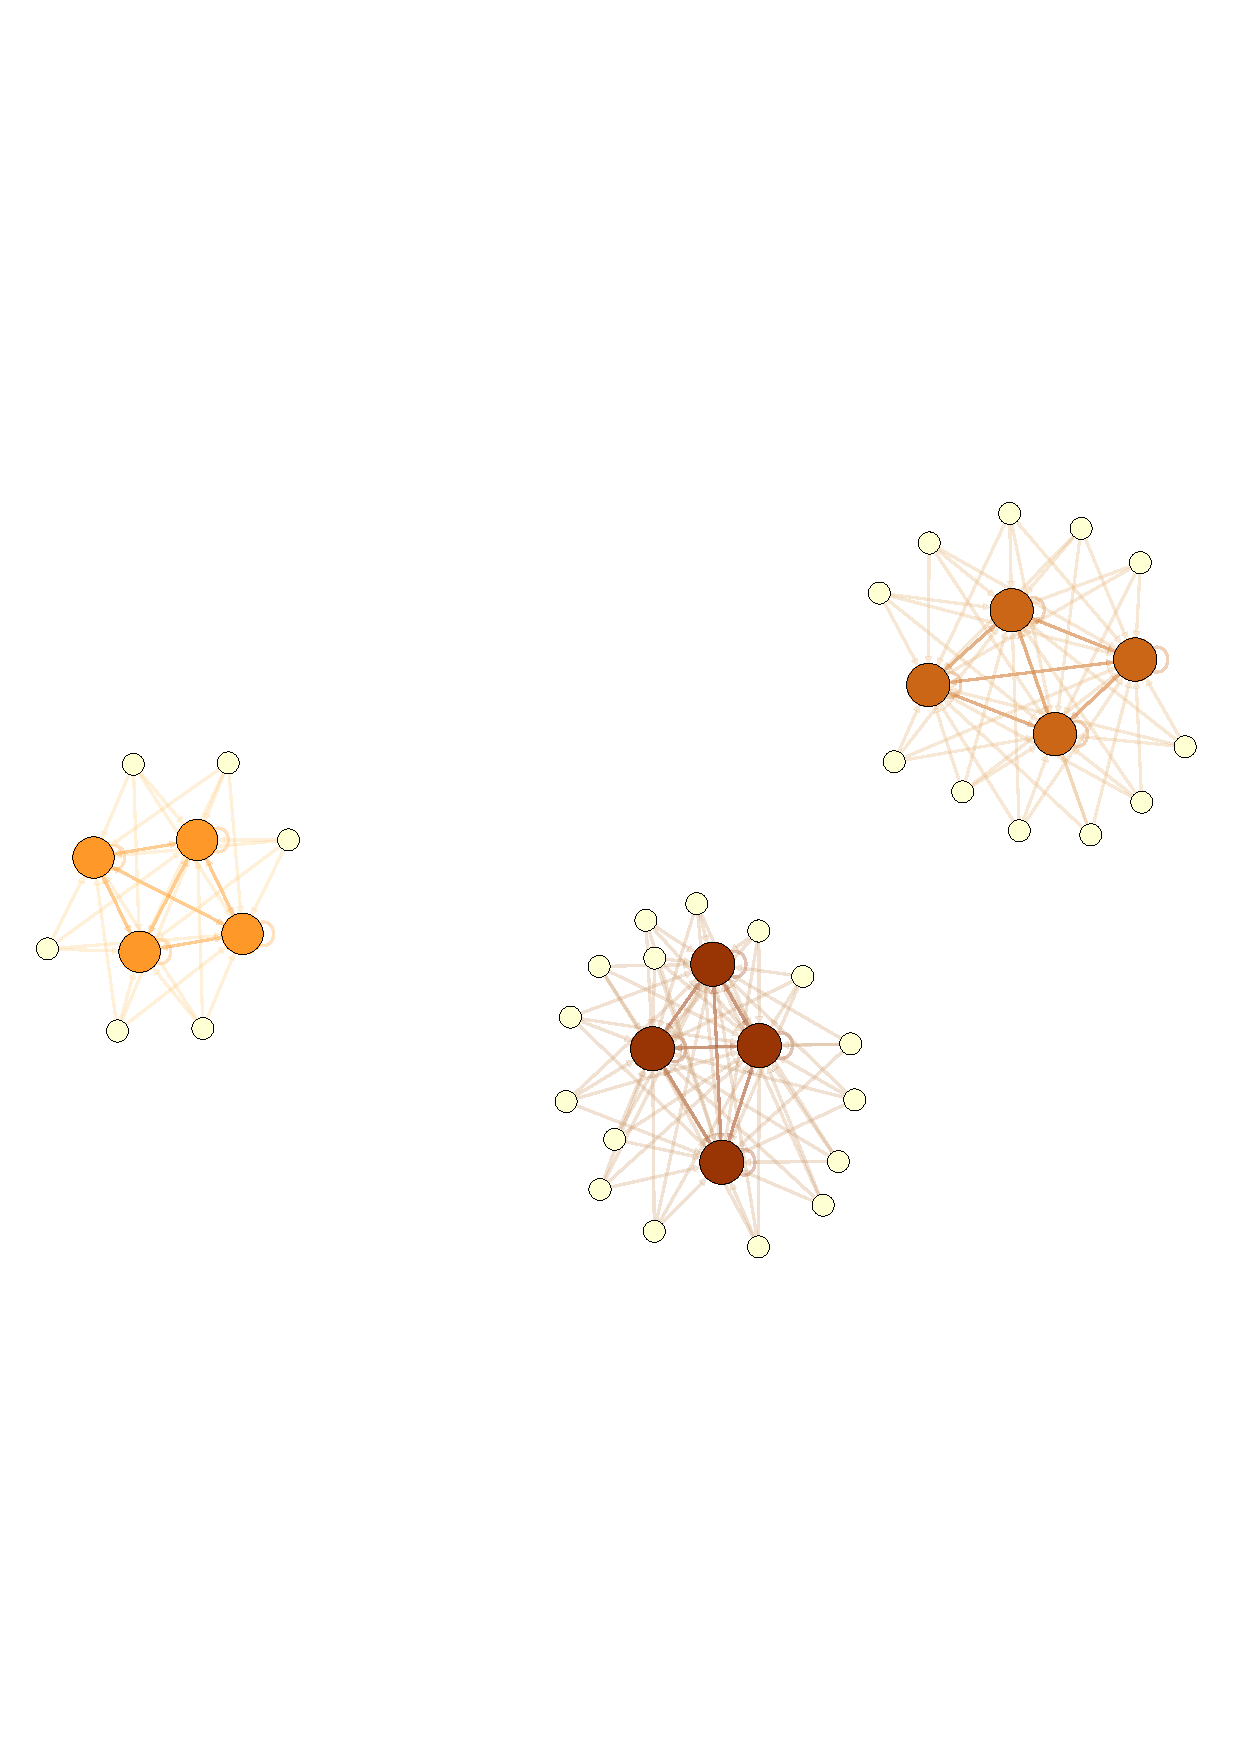
\includegraphics[width=\textwidth,
		trim = 0 220 0 220, clip
		]{imagenes/disconexo.pdf}
	\caption{\label{fig:disconexo} El sistema actual le da mucho peso a pocos hoteles y además no permite llegar de un grupo a otro.}
\end{figure}

Para modelar las recomendaciones del sistema con una red hay que tener algunas consideraciones. Por un lado, a cada hotel le asignamos un ordenamiento de los demás hoteles dentro de un cierto radio vía el \emph{score}. Sin embargo, utilizar esto como peso para los arcos no es muy realista, puesto que el \emph{score} está en una escala sin ninguna interpretación. Una mejor alternativa es poner como arcos únicamente las 5 mejores recomendaciones de cada hotel, dado que serán los que los clientes verán directamente, sin tener que bajar la lista. Dado que no tenemos información sobre la importancia de cada posición en la lista, supondremos que son iguales, esto es, todos los arcos tendrán el mismo peso.

Una manera de evaluar la importancia de los nodos sería utilizando su grado de entrada. Sin embargo, esta métrica tiene la desventaja de que da información puramente local. Es decir, si conocemos el grado de entrada, podemos saber cuántos hoteles le apuntan directamente a uno dado, pero no sabemos si hay una tendencia de la gráfica como conjunto a tender a esos nodos. Por esta razón utilizaremos mejor el PageRank, que sí aporta información global, para evaluar la importancia de los nodos.

\section{Análisis de la red}

Dado que la gráfica resultante de las recomendaciones de los miles de hoteles de Best Day sería poco informativa en un entorno no interactivo, optamos por presentar los resultados del análisis en algunas zonas de interés. Primero haremos un análisis a una escala de varios destinos y posteriormente nos acercaremos a ver con más detalle uno solo.

Analizamos varios destinos importantes de México en la gráfica (\ref{fig:destinos}). En este caso, el tamaño de los nodos está dado por su PageRank, por lo que los nodos son más importantes mientras más grandes son, mientras que los colores representan el destino de cada hotel. Esta representación del sistema de recomendación transparenta algunas de las ventajas que tiene. En primer lugar, vemos que la importancia de los nodos está mucho más repartida que en la gráfica de ejemplo del sistema actual. Aunque hay algunos nodos grandes, no son los únicos importantes en la gráfica. En términos de las características que buscábamos al principio, esto equivale a que el sistema sea más \emph{creativo} e \emph{inteligente}, puesto que no recomendará siempre lo mismo. Además de ello, la gráfica de cada destino es débilmente conexa, lo que dificulta que al sistema ``se le acaben las ideas''; veremos esto a mayor detalle en una figura posterior. Otra ventaja evidente es que los destinos muy cercanos pueden estar conectados, como en el caso de los que están en Quintana Roo. Es interesante notar que si hay varios destinos en cadena, se puede llegar a lugares muy lejanos si se explora lo suficiente. Por ejemplo, se puede llegar de Cancún a Tulum, incluso a pesar de que están a 130 km de distancia. Esto puede ser una ventaja porque un cliente que no tiene un destino decidido puede explorar alternativas en una zona más amplia que el destino que se le había ocurrido inicialmente. Esto se puede interpretar como que el sistema tiene cierto \emph{ingenio} y capacidad de encontrar soluciones \emph{out-of-the-box}.
\begin{figure}[ht]
	\centering
	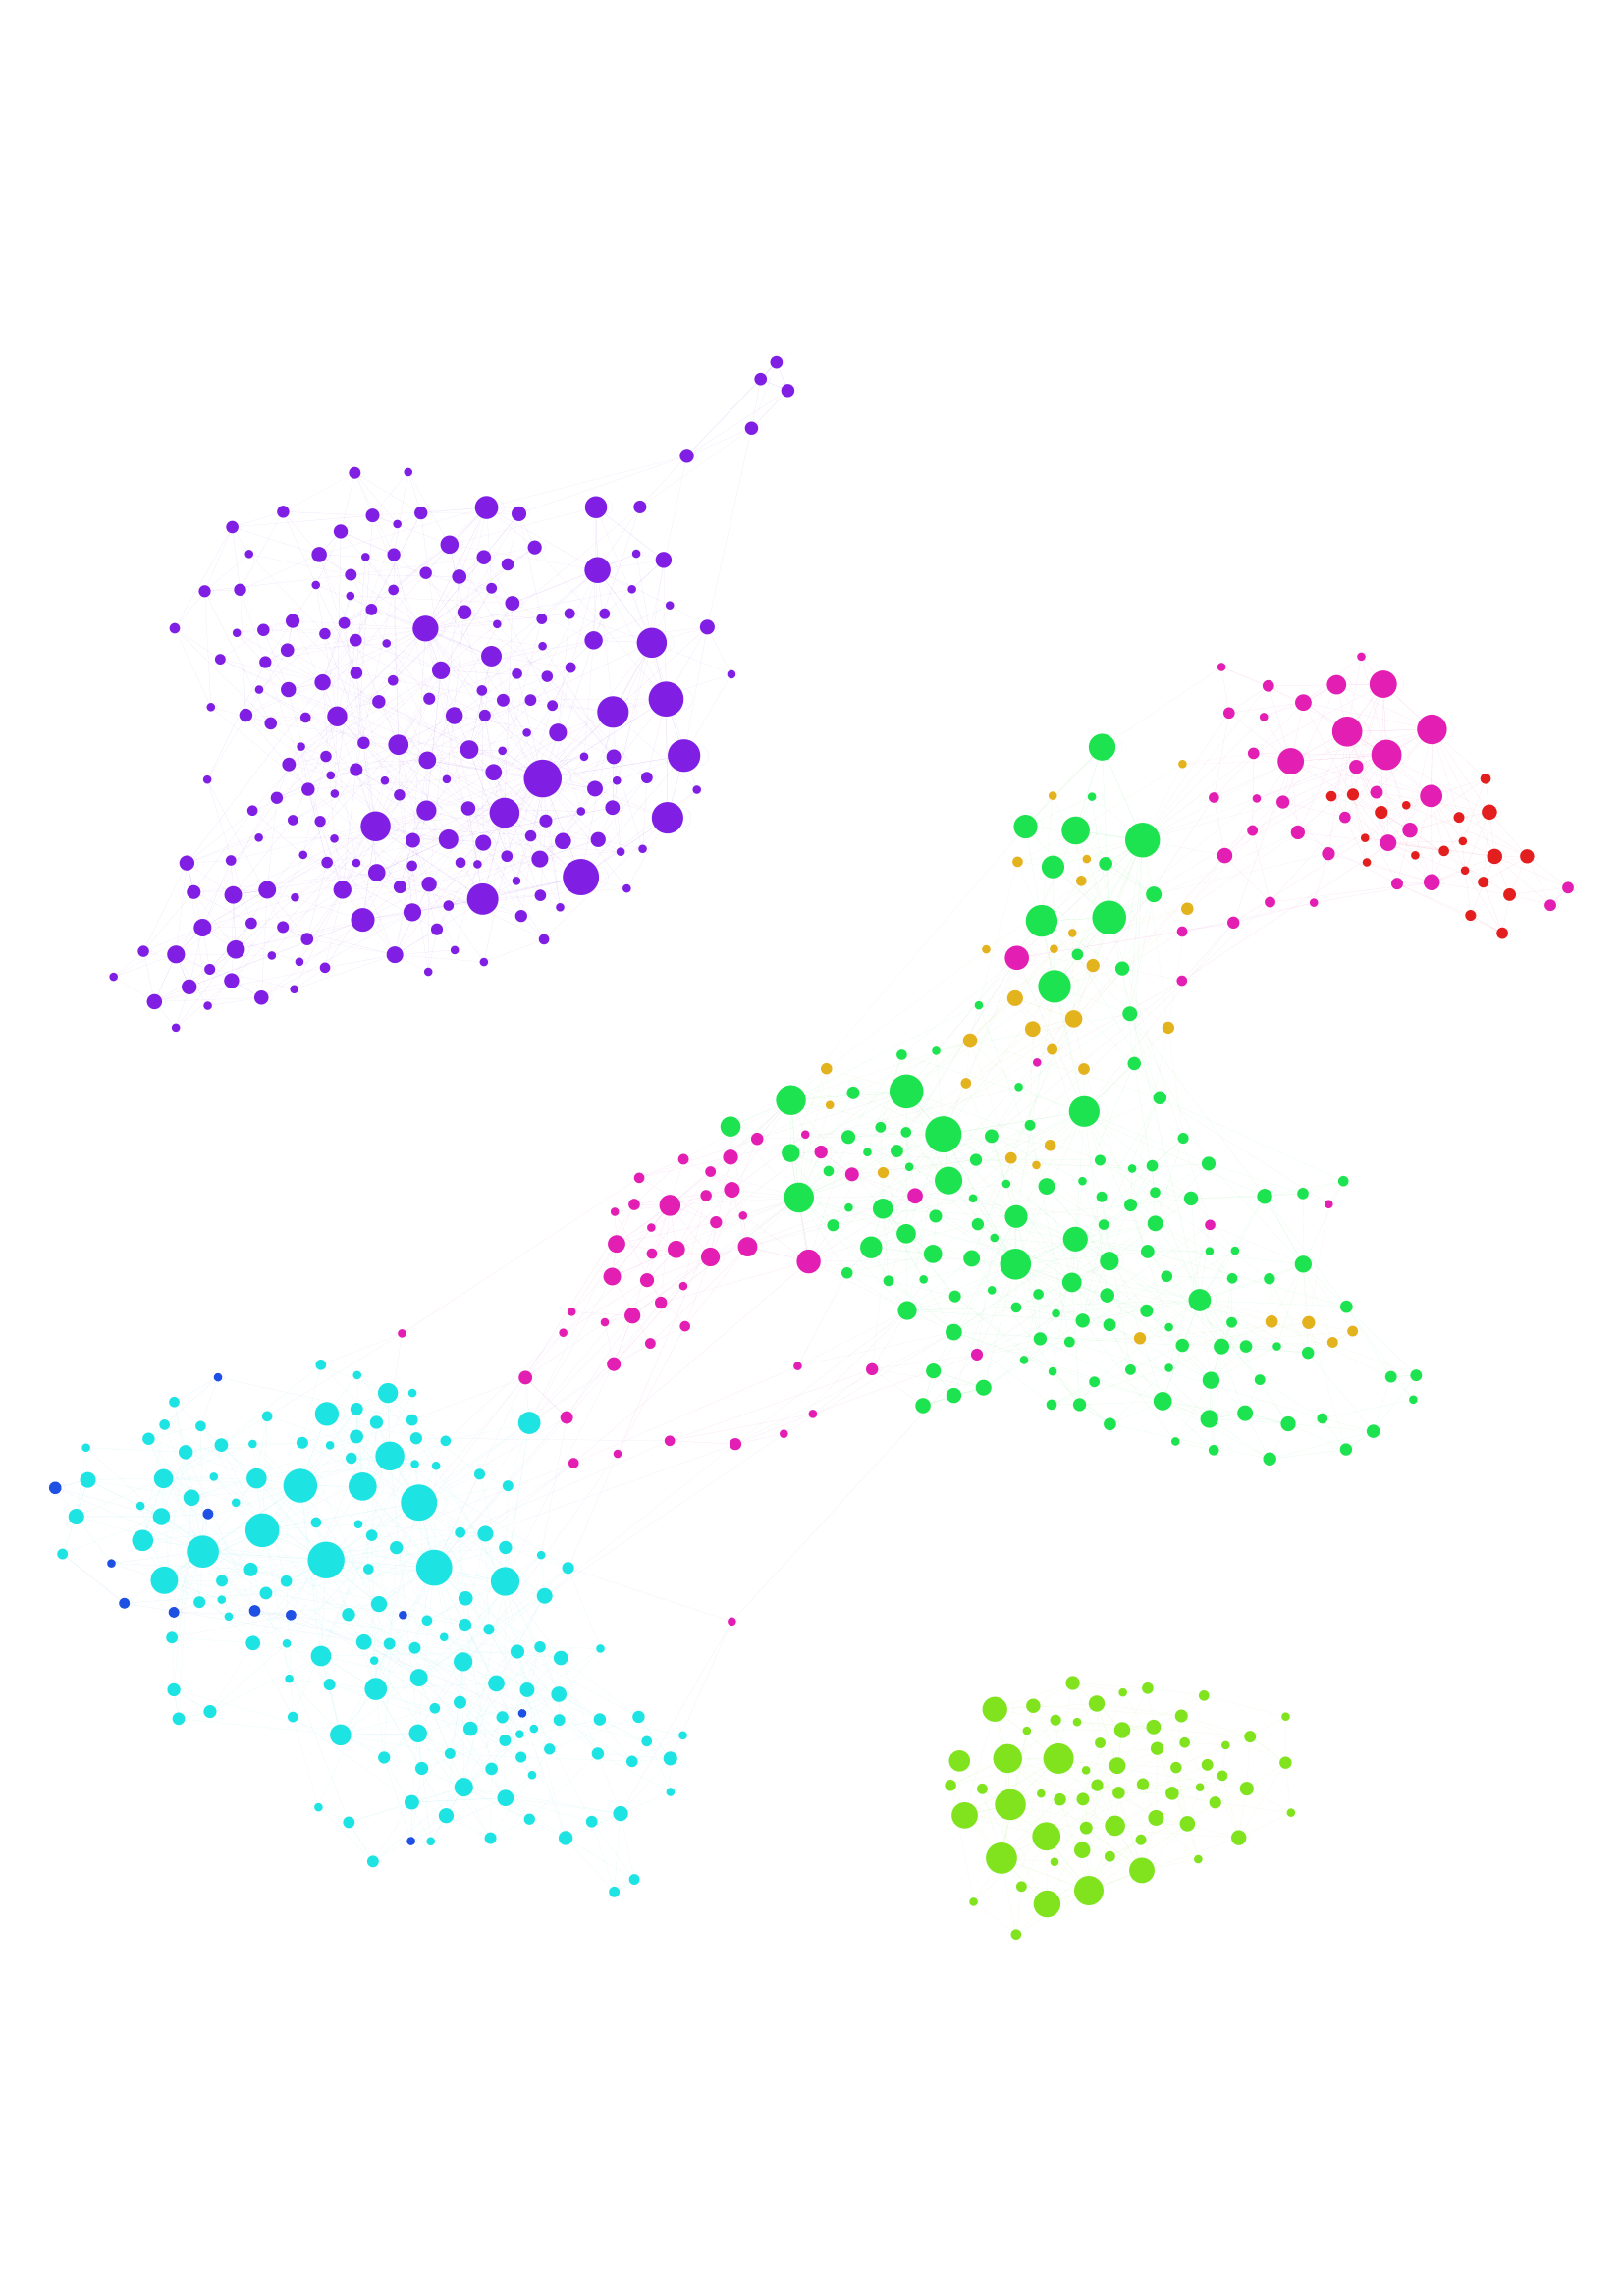
\includegraphics[width=0.7\textwidth,
		trim = 0 300 0 300, clip]{imagenes/destinos2.png}
	\caption{\label{fig:destinos} Red para diversos destinos: Ciudad de México (azul-morado), Cancún (turquesa), Playa del Carmen (verde), Riviera Maya (fucsia), Isla Mujeres (azul), Cozumel (naranja), Tulum (rojo) y Cuernavaca (verde-amarillo). El tamaño de los nodos está dado por el PageRank.}
\end{figure}

Si ahora nos acercamos a un destino en particular, podremos descubrir otras cosas interesantes. Dado que Cancún es el destino principal de Best Day, ahí es donde enfocaremos nuestro análisis. La figura (\ref{fig:cancun}) ilustra qué hoteles son los más importantes en esta zona. En este caso, el tamaño representa el PageRank de los hoteles, por lo que un hotel con un nodo grande tendrá mayor probabilidad de ser elegido al azar utilizando únicamente las recomendaciones. Es inmediato ver que esta gráfica está mucho más balanceada que las estrellas que aparecían en la (\ref{fig:disconexo}), puesto que es al menos débilmente conexa. Además, los hoteles tienen varios niveles de importancia en lugar de que haya unos pocos que la acumulen toda.

\begin{figure}[ht]
	\centering
	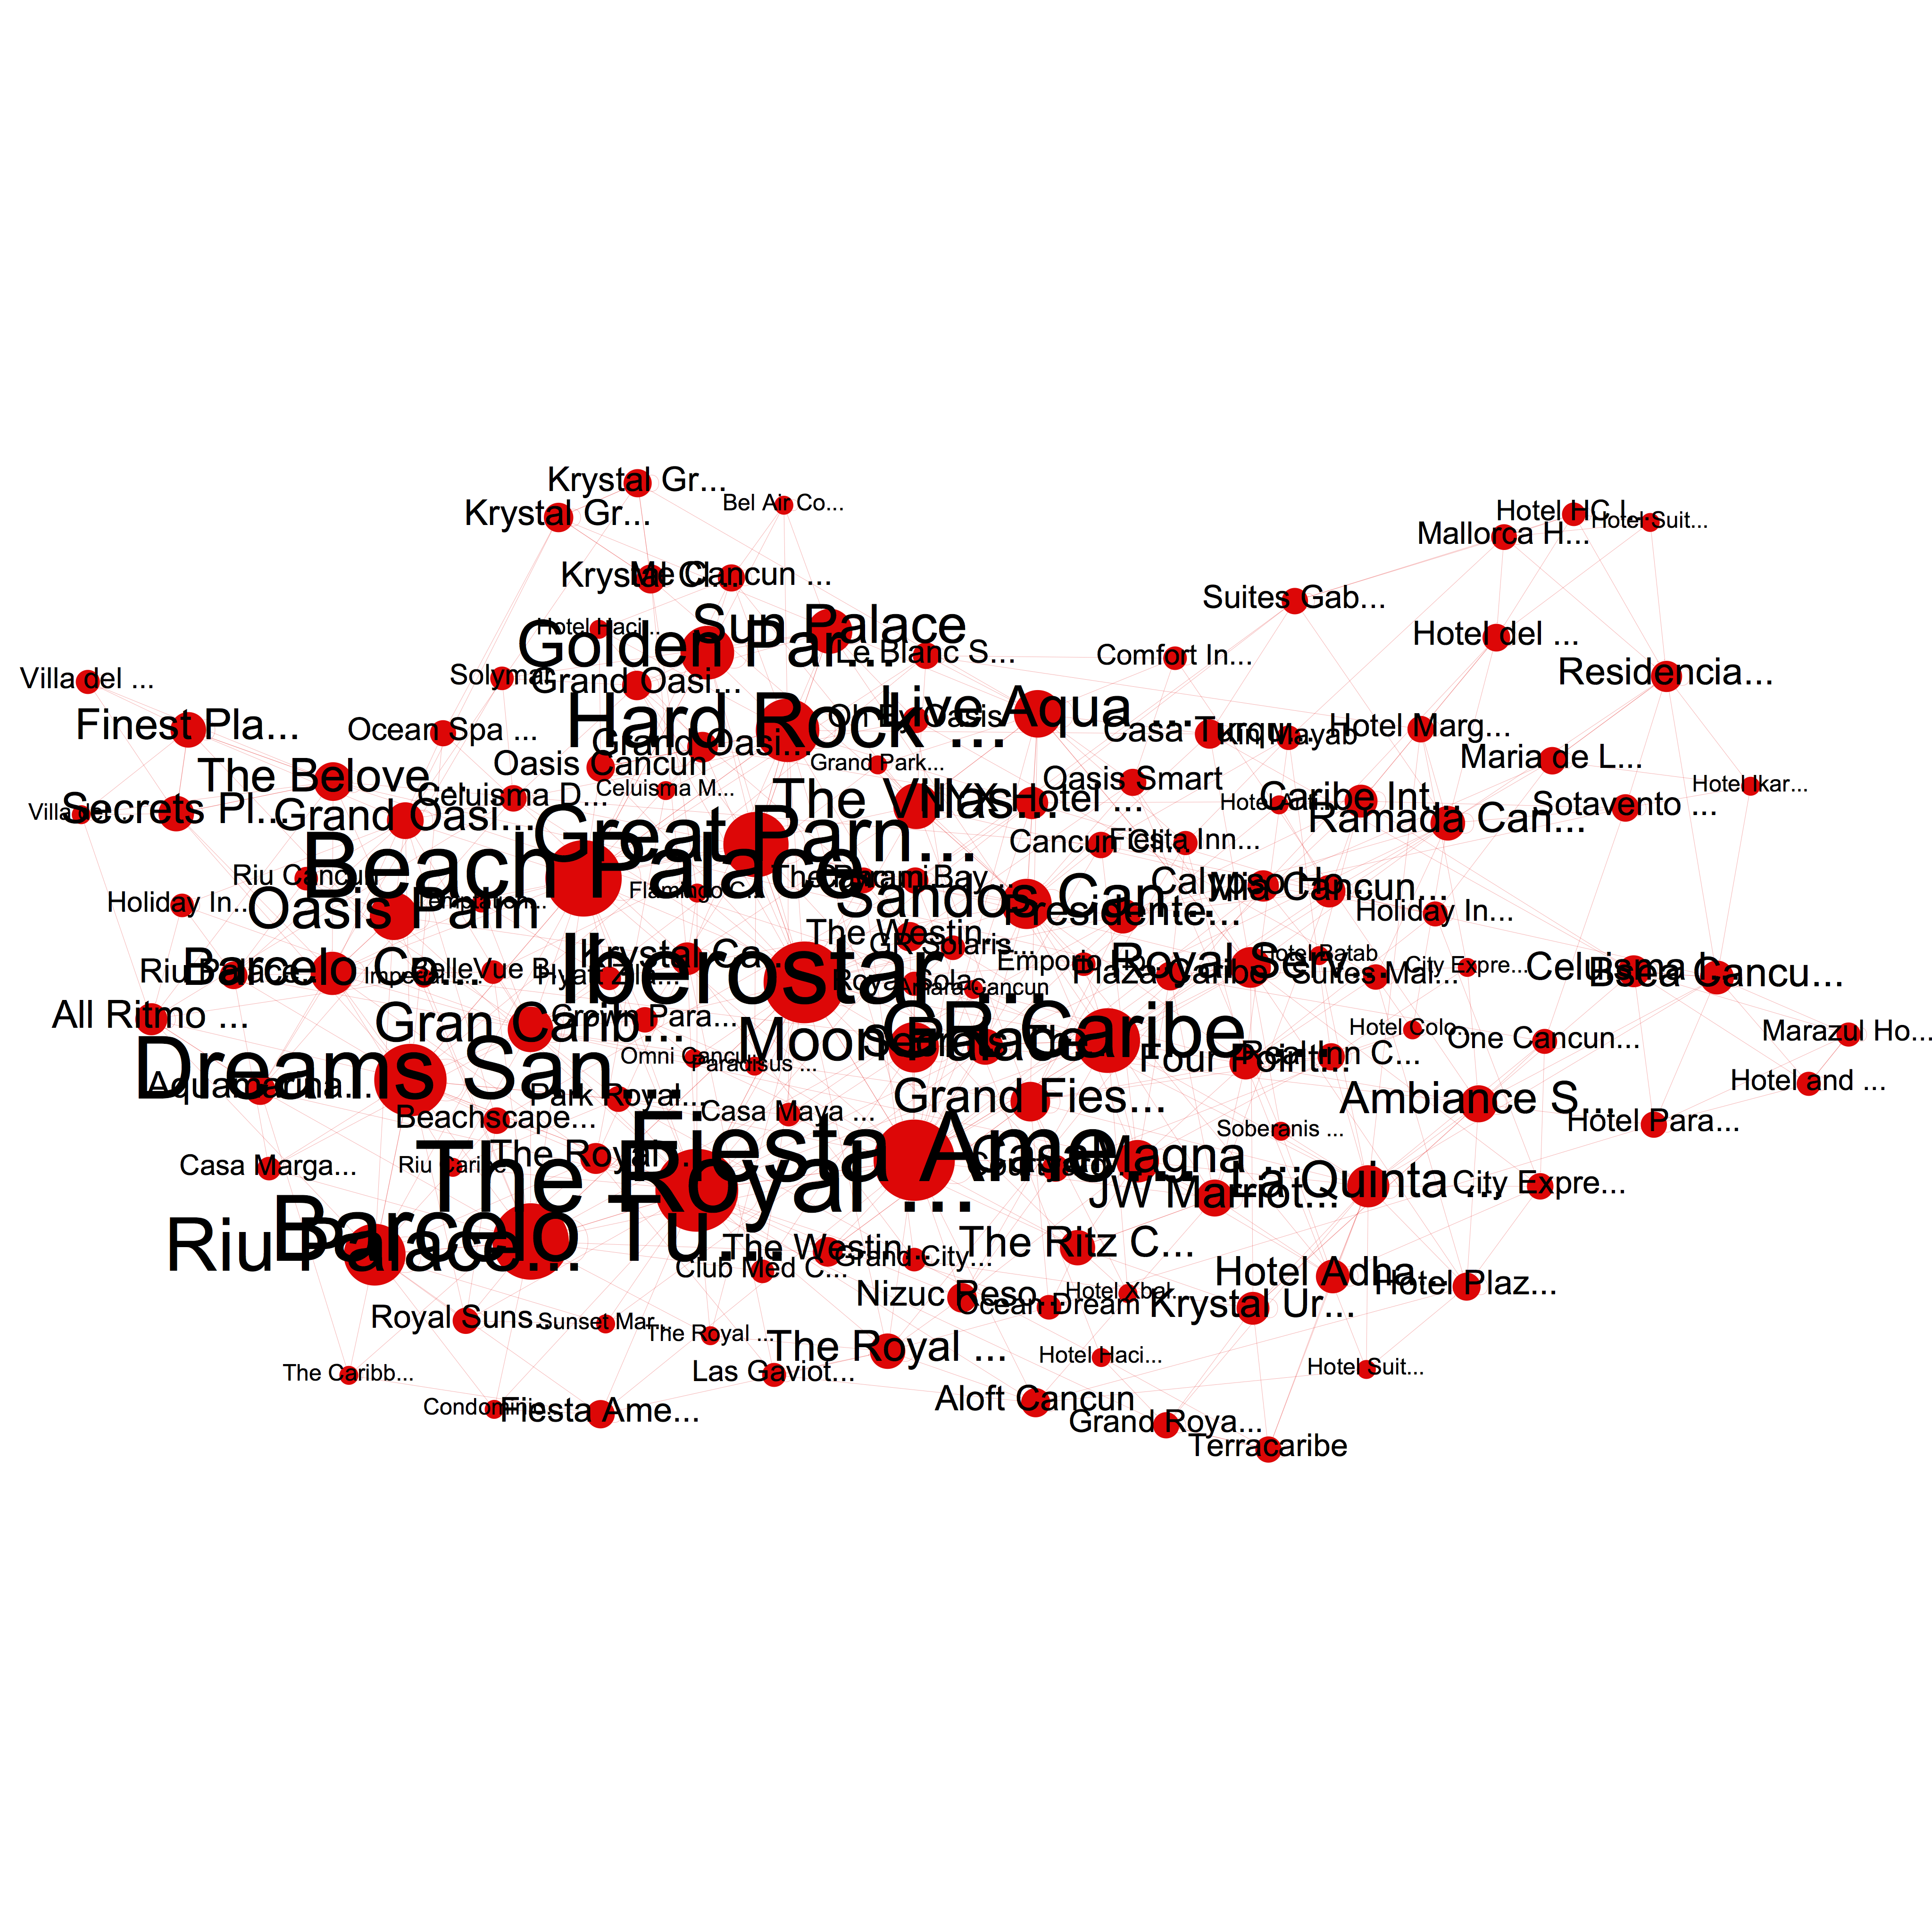
\includegraphics[width=0.70\textwidth, angle=0,
		trim = 0 900 0 900, clip]{imagenes/cancun.png}
	\caption{\label{fig:cancun} Hoteles en Cancún. La importancia (PageRank) está dada por el tamaño de los nodos. Sin contar los nodos inaccesibles, el diámetro de esta gráficaes de 7 pasos y la distancia promedio entre nodos es de 3.3.}
\end{figure}

Ya con una idea de qué hoteles son los más relevantes podemos hacer otro tipo de análisis. Las figuras (\ref{fig:cancun_laquinta}) y (\ref{fig:cancun_iberostar}) también incluyen únicamente hoteles en Cancún y el tamaño de sus nodos está dado de la misma manera. Sin embargo, en estos casos el color corresponde al número de pasos que se requiere para llegar de un hotel determinado a los demás. En particular, el hotel más oscuro es el de origen y el color se va degradando conforme más y más pasos se requiera para llegar a los demás. Los hoteles en gris no son accesibles desde el hotel original mediante las primeras cinco recomendaciones de los hoteles\footnote{Cabe notar que en realidad son cuatro recomendaciones efectivas, puesto que cada hotel aparece en el primer lugar de su propia lista.}. Este hecho muestra que, si bien el sistema nuevo es más flexible que el anterior, no puede hacer saltos lógicos demasiado aventurados, incluso en varias etapas. Sin embargo, este hecho no necesariamente es negativo, puesto que, en la mayoría de los casos, los clientes sólo estarán interesados en una parte específica del espectro de hoteles en una zona.

Como podemos ver en la gráfica (\ref{fig:cancun_laquinta}), de un hotel citadino y de negocios como La Quinta Inn and Suites podemos llegar sin problemas tanto a otros hoteles similares como a hoteles populares en la zona si damos \emph{click} en las recomendaciones adecuadas. Similarmente, la gráfica (\ref{fig:cancun_iberostar}) muestra las posibilidades que se tiene empezando en el hotel Iberostar Cancún. Es claro ver que en el primer caso hay una mayor cantidad de hoteles accesibles que en el segundo, al menos mediante las primeras cinco recomendaciones. Esto se debe a que usualmente es más fácil explorar las regiones remotas de la red empezando en un hotel poco reconocido que en uno popular. Esto ocasiona que el asesor electrónico reconozca la calidad de ciertos hoteles y tenga una tendencia a llevar al cliente a ellos. 
\begin{figure}[h!t]
	\centering
	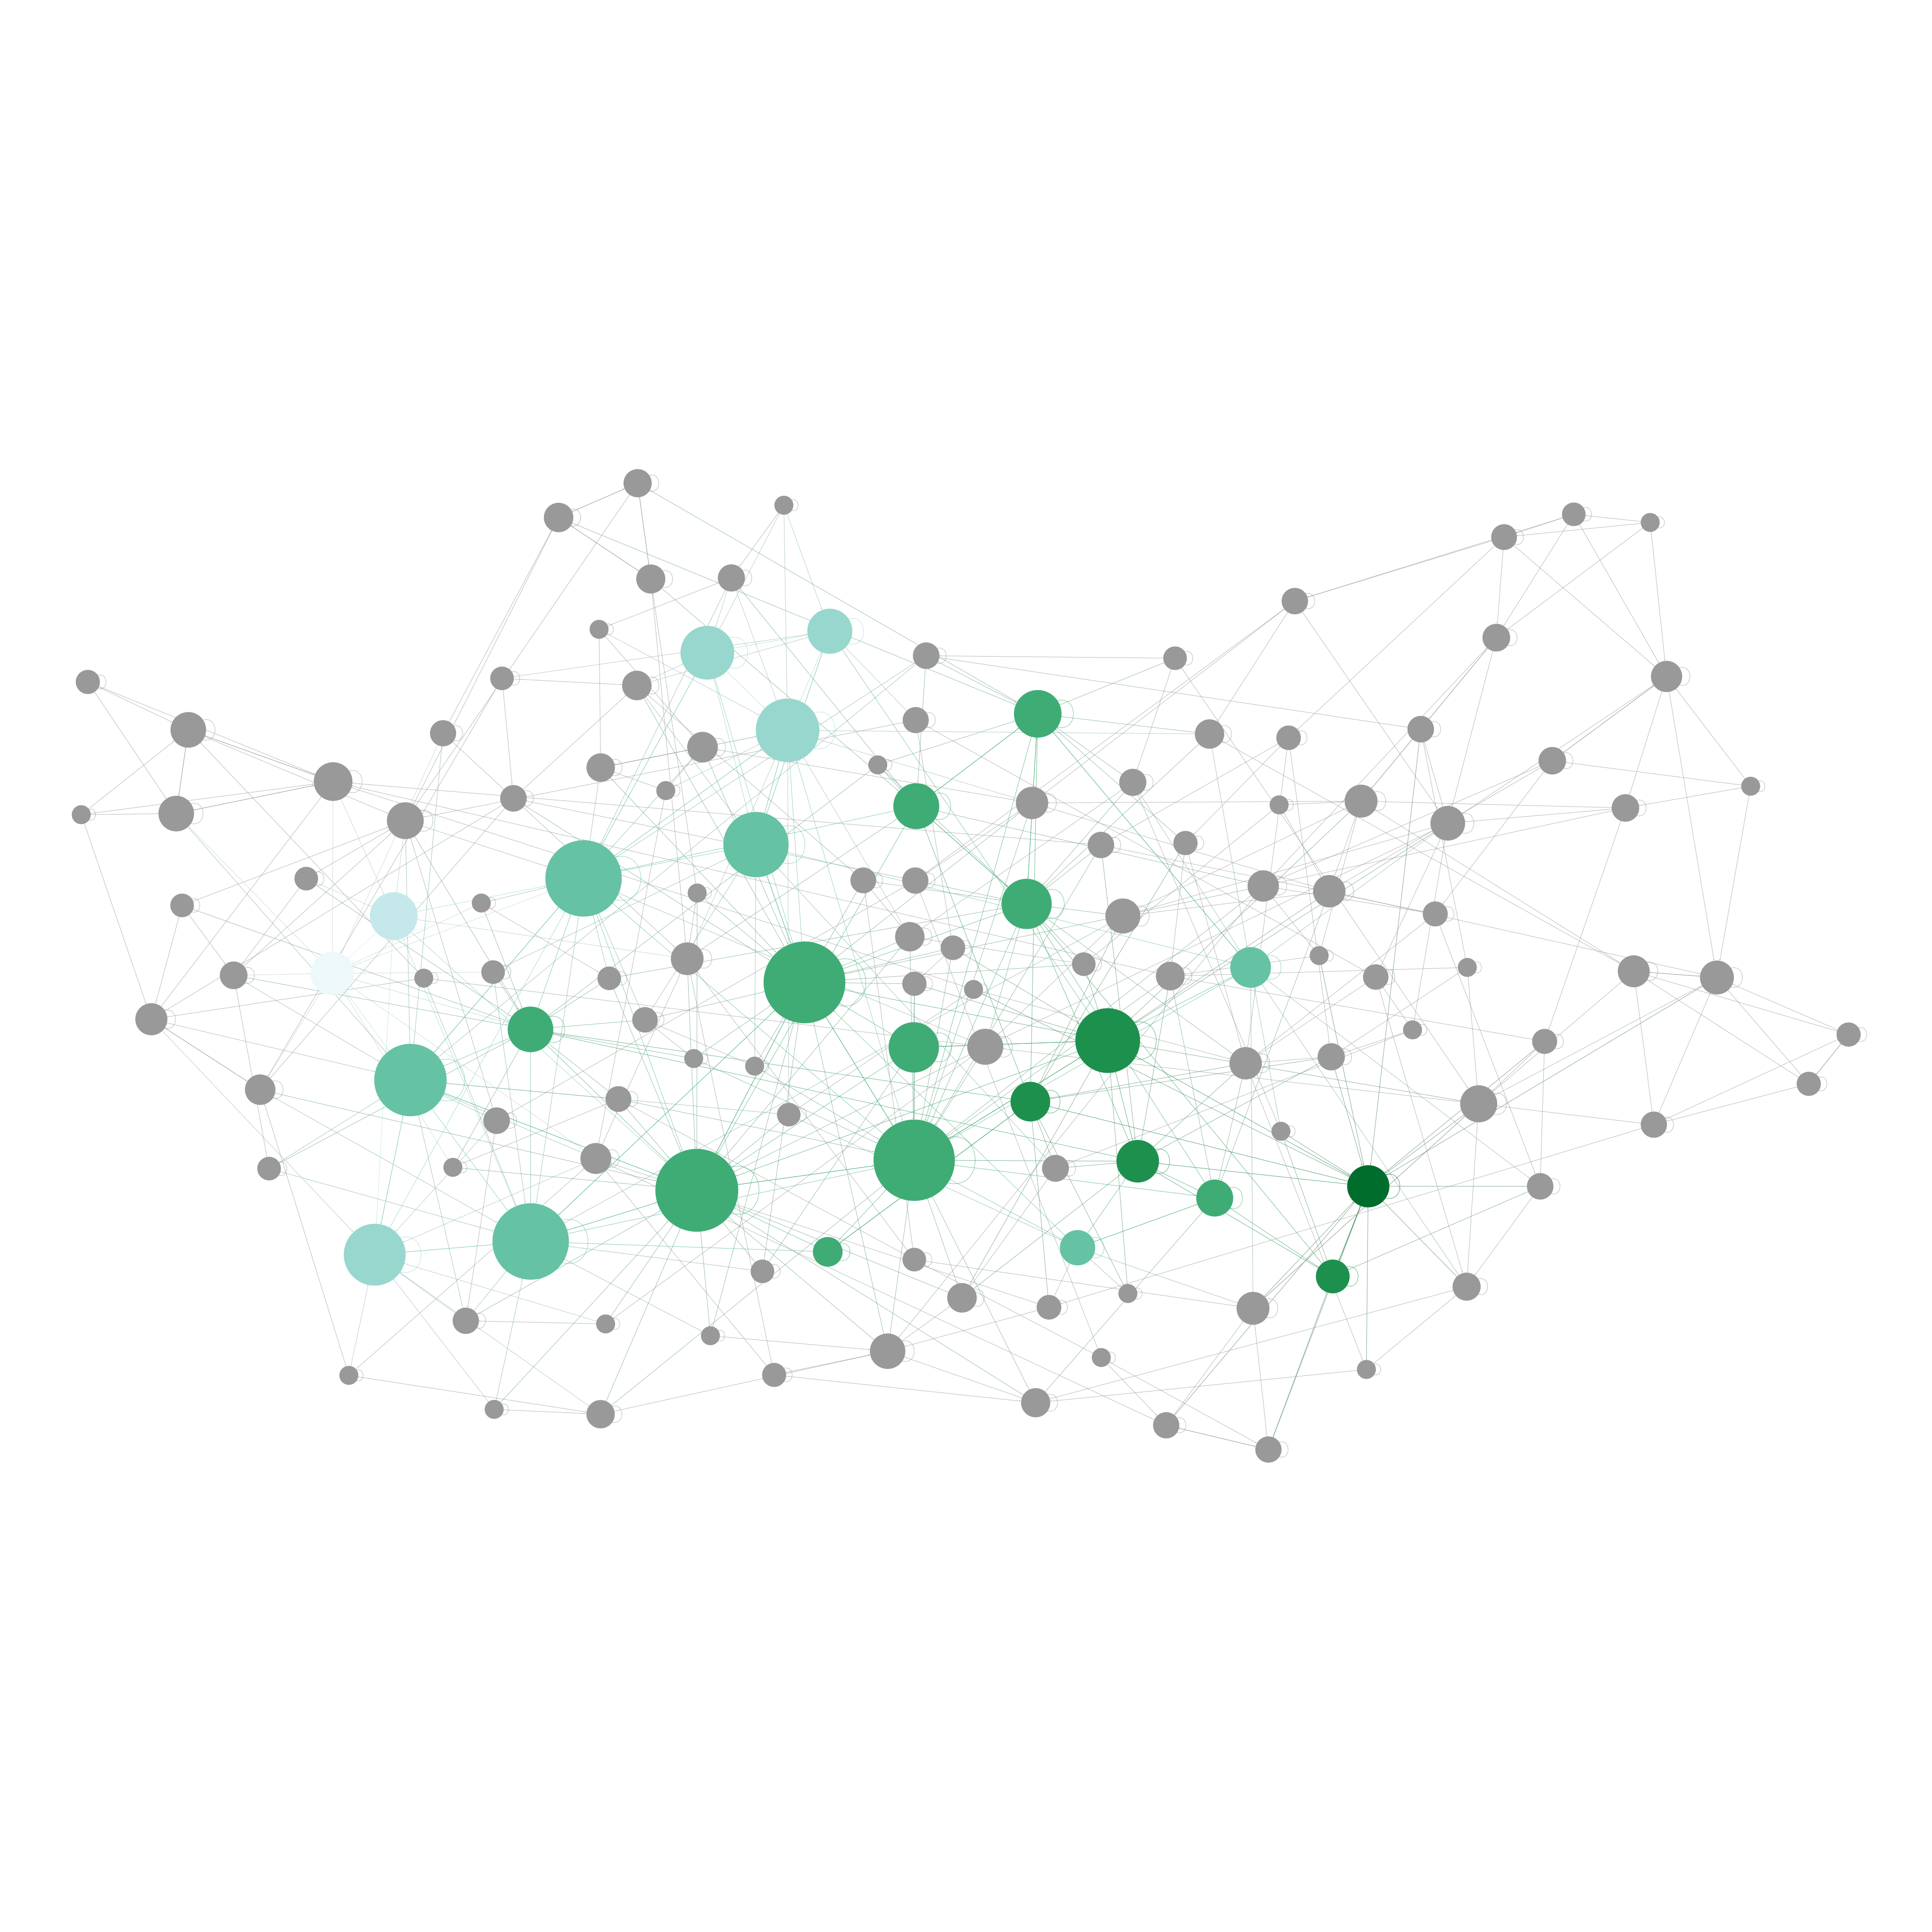
\includegraphics[width=0.9\textwidth, angle=0,
		trim = 100 900 100 900, clip]{imagenes/cancun_laquinta2.png}
	\caption{\label{fig:cancun_laquinta} Tamaño: PageRank. Color: Más oscuro implica mayor cercanía (en recomendaciones) al hotel La Quinta Inn and Suites.\\\vspace*{1cm}}
	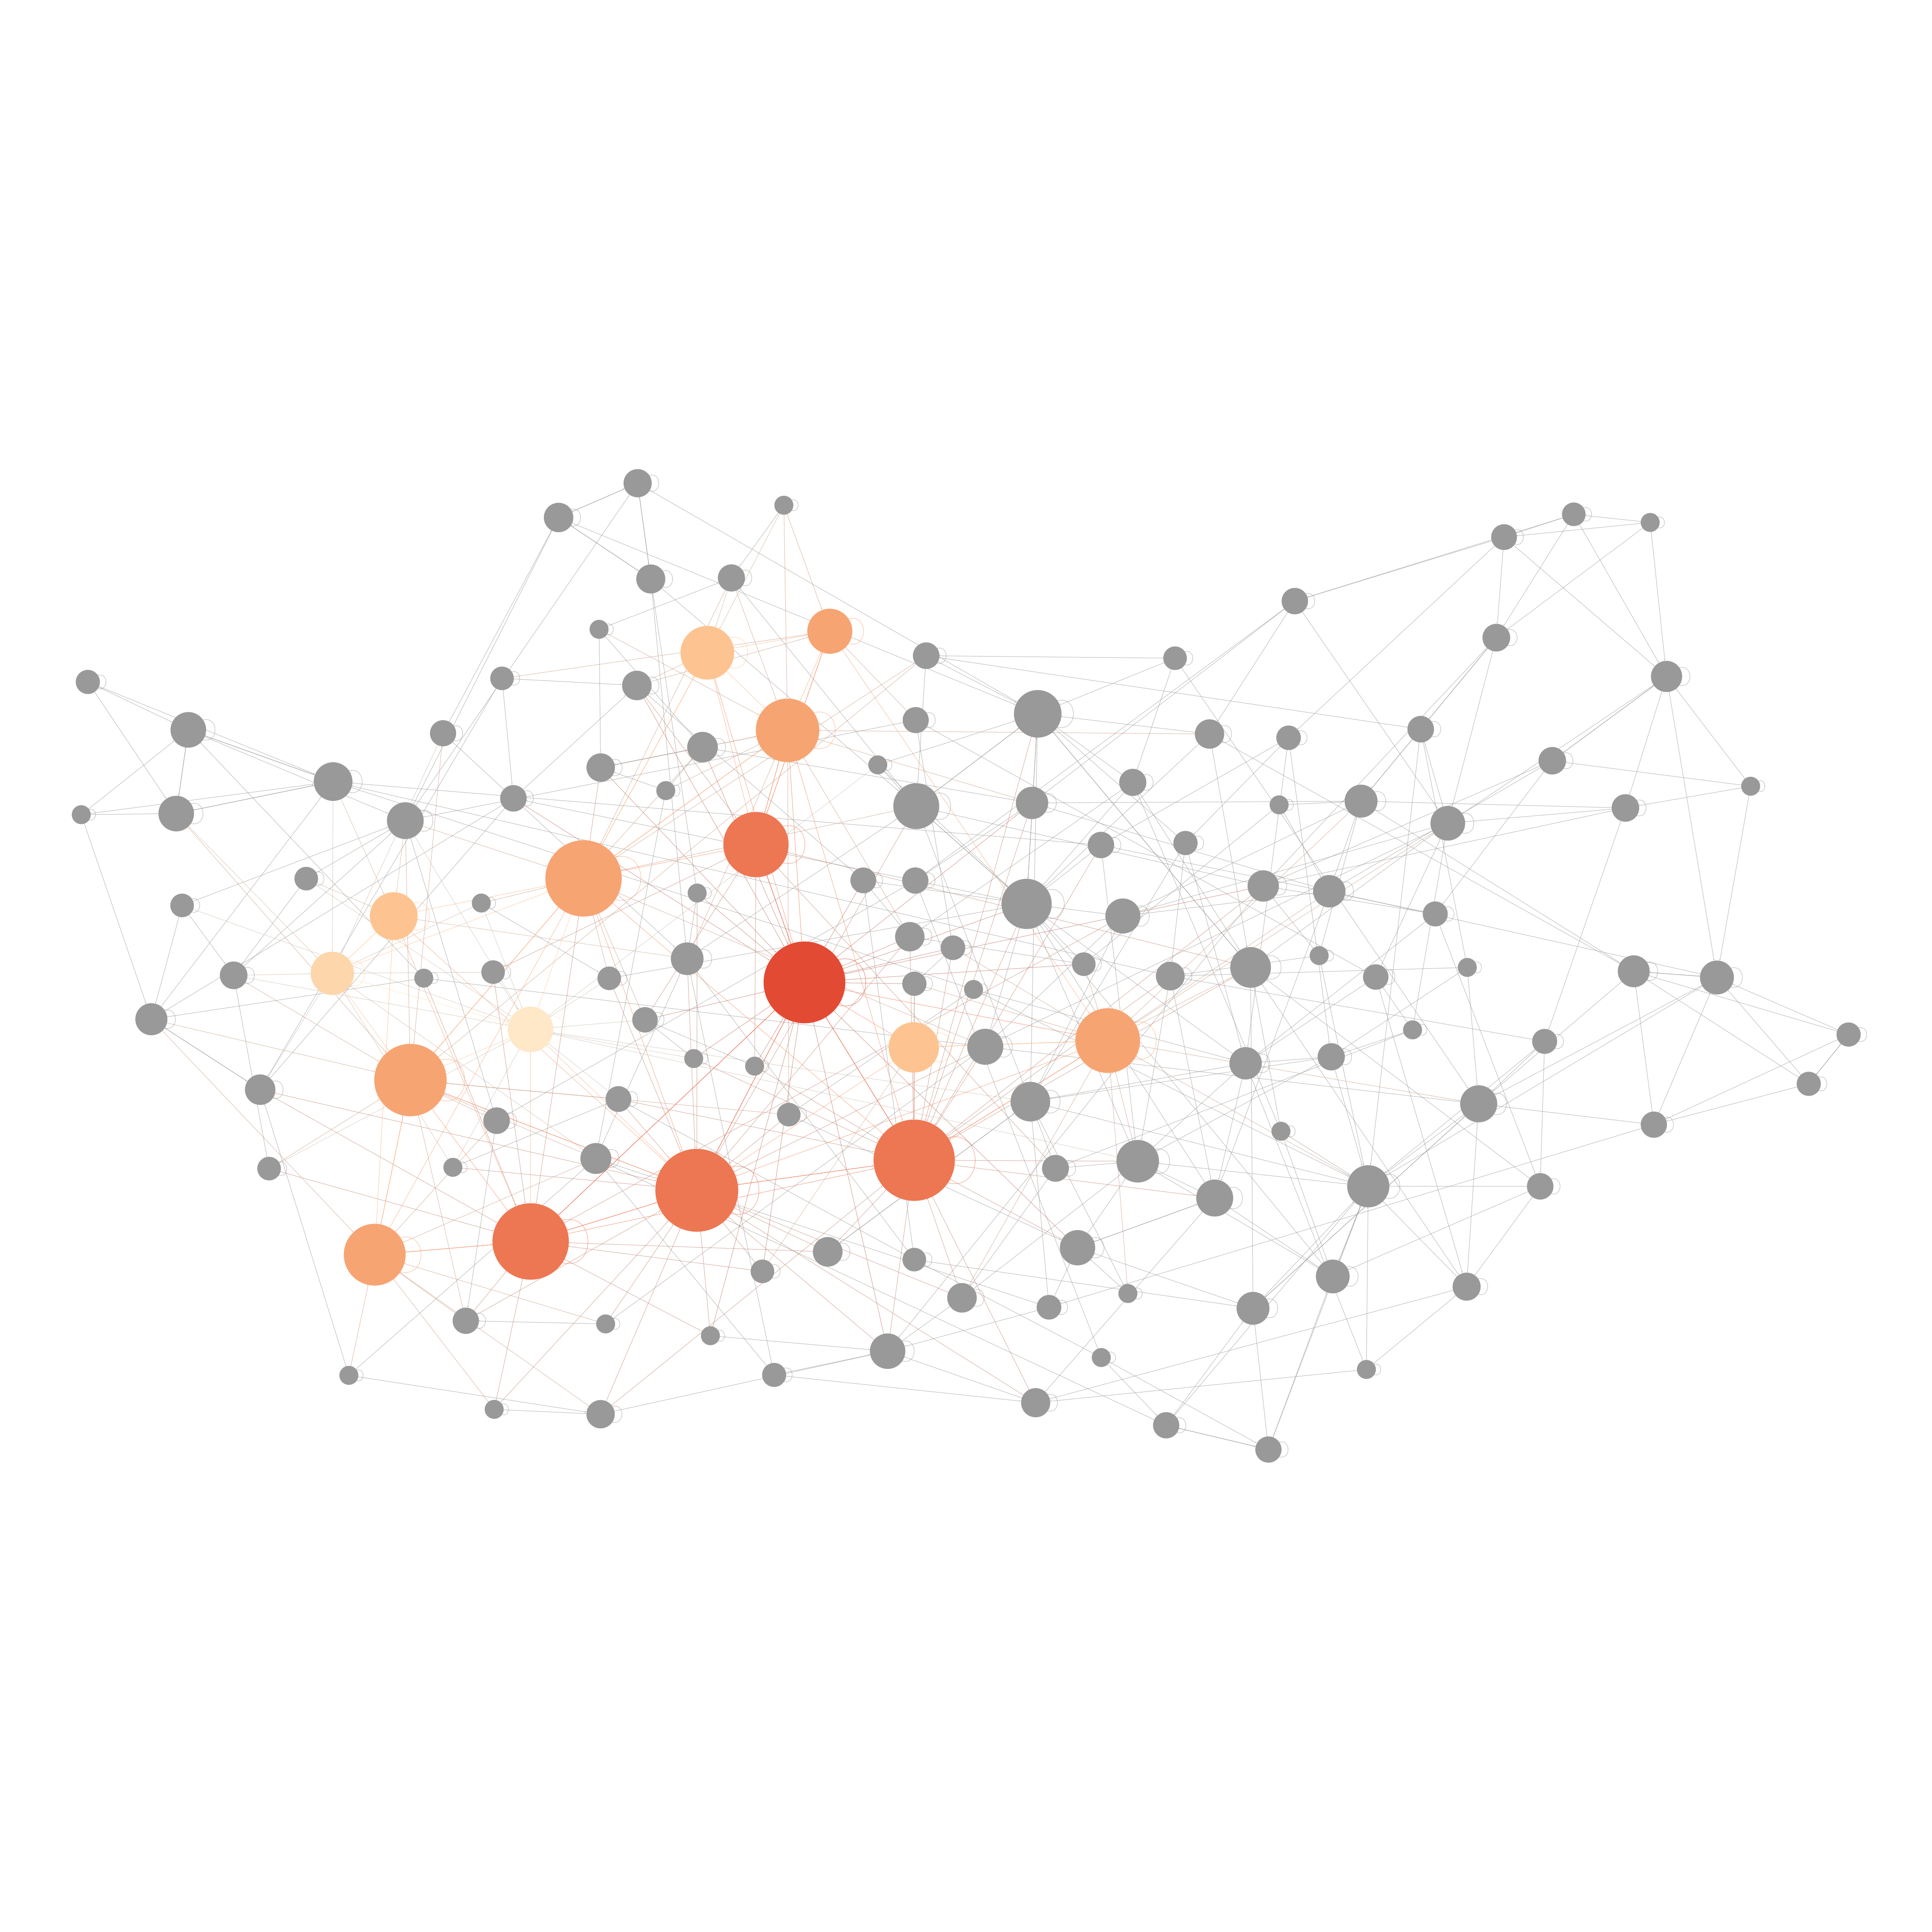
\includegraphics[width=0.9\textwidth, angle=0,
		trim = 100 900 100 900, clip]{imagenes/cancun_iberostar2.png}
	\caption{\label{fig:cancun_iberostar} Tamaño: PageRank. Color: Más oscuro implica mayor cercanía (en recomendaciones) al hotel Iberostar Cancún.}
\end{figure}

\clearpage
\section{Conclusiones del análisis de redes}

Si bien el sistema que construimos tiene muchas propiedades favorables, hay que tener algunas cosas en mente. Para ello, concluiremos nuestro análisis de redes con los siguientes puntos clave.

Antes que nada, hay que notar que si bien el sistema de recomendación fue construido de manera cuidadosa, sus bondades dependen de las características particulares de la zona, por lo que no hay garantía de que se comportará de manera óptima en todos lados. Por ejemplo, no hay razón alguna para pensar que todos los hoteles aparecerán en las recomendaciones de algún otro hotel. Es decir, es posible que nadie recomiende a un hotel en particular. Habrá que tener cuidado con esto y monitorear que no afecte el desempeño del sistema, aunque creemos que en la práctica sería difícil que esto representara un problema.

Otro aspecto que hay que tener en cuenta es que, aunque el precio no está restringido por abajo, la estructura de la red tiene cierta tendencia a llevar al cliente a los hoteles con PageRank alto. Habrá que observar el cambio en el comportamiento de los clientes para determinar si esto afecta negativamente a los hoteles menos comunes. Nuestra principal preocupación es que demasiados acaben en las mismas opciones siempre, aunque dudamos que el problema sea ni cercanamente tan grave como con el sistema actual.

Finalmente, en las redes anteriores hicimos dos grandes supuestos que no necesariamente se cumplirán en la práctica: (1) que los clientes sólo ven las primeras cinco recomendaciones (cuatro de ellas distintas al original), y (2) que los clientes eligen una recomendación al azar y con la misma probabilidad. El primer supuesto no se cumplirá en la práctica porque los clientes tendrán más alternativas si ven más elementos de la lista de recomendaciones. Este hecho es ventajoso para el sistema porque ayudará, al menos en parte, a que haya menos hoteles que nadie recomiende. El segundo supuesto tampoco se cumplirá porque hay otros factores que motivan a un cliente a seleccionar una recomendación, como por ejemplo el precio, la foto (\emph{thumbnail}) que se le presenta en la página o incluso el nombre del hotel. Se podría hacer un análisis exhaustivo usando herramientas estadísticas que analicen el comportamiento de la página, pero no estamos seguros de que el impacto sería lo suficientemente importante para justificar dicho análisis.

%--------------------------------------------------------------

\chapter{Resultados prácticos y conclusiones} \label{cap:5}

\section{Desempeño de la página web}

El análisis de redes de del capítulo \ref{cap:4} evalúa el sistema de recomendación desde un punto de vista hipotético, en el sentido de que nos permite ver qué cosas \emph{puede} o no hacer el sistema. Por ejemplo, ilustra desde qué nodos de la gráfica podemos llegar a cuáles otros, cuáles son más importantes, etc. Sin embargo, el análisis teórico de la red debe ser complementado con uno de su desempeño en el mundo real, que en este caso corresponde con el de la página web de Best Day. Utilizamos la herramienta Google Analytics\footnote{Más información en la página incluida en la bibliografía, \cite{analytics}.} para obtener las diversas métricas de interés que analizaremos en esta sección.

Dado que estamos presentando una versión nueva de un sistema que ya existía, nos gustaría comparar su desempeño contra la versión actual y no tanto en términos absolutos. Para hacerlo, nos basaremos en las series de tiempo de las diversas métricas, fijándonos qué pasó antes y después de que subiéramos el nuevo sistema a producción. Lo haremos para las sesiones que fueron asistidas por el sistema de recomendación (i.e. que dieron \emph{click} en alguna recomendación), para los siguientes indicadores:
\begin{enumerate}
	\item \emph{Número de \glspl{visita}} realizadas a la página.
	\item \emph{\Gls{bouncerate}}, es decir, la proporción de clientes que entró a la página y se salió sin dar \emph{click} a ninguna liga.
	\item \emph{Duración promedio de la sesión} del cliente en la página.
	\item \emph{\Gls{conversionrate}}, que es la proporción de clientes que compraron algo una vez habiendo entrado a la página.
	\item \emph{Número promedio de páginas} visitadas durante la sesión
	\item \emph{Monto promedio} de cada transacción.
\end{enumerate}

\begin{figure}[ht]
	\centering
	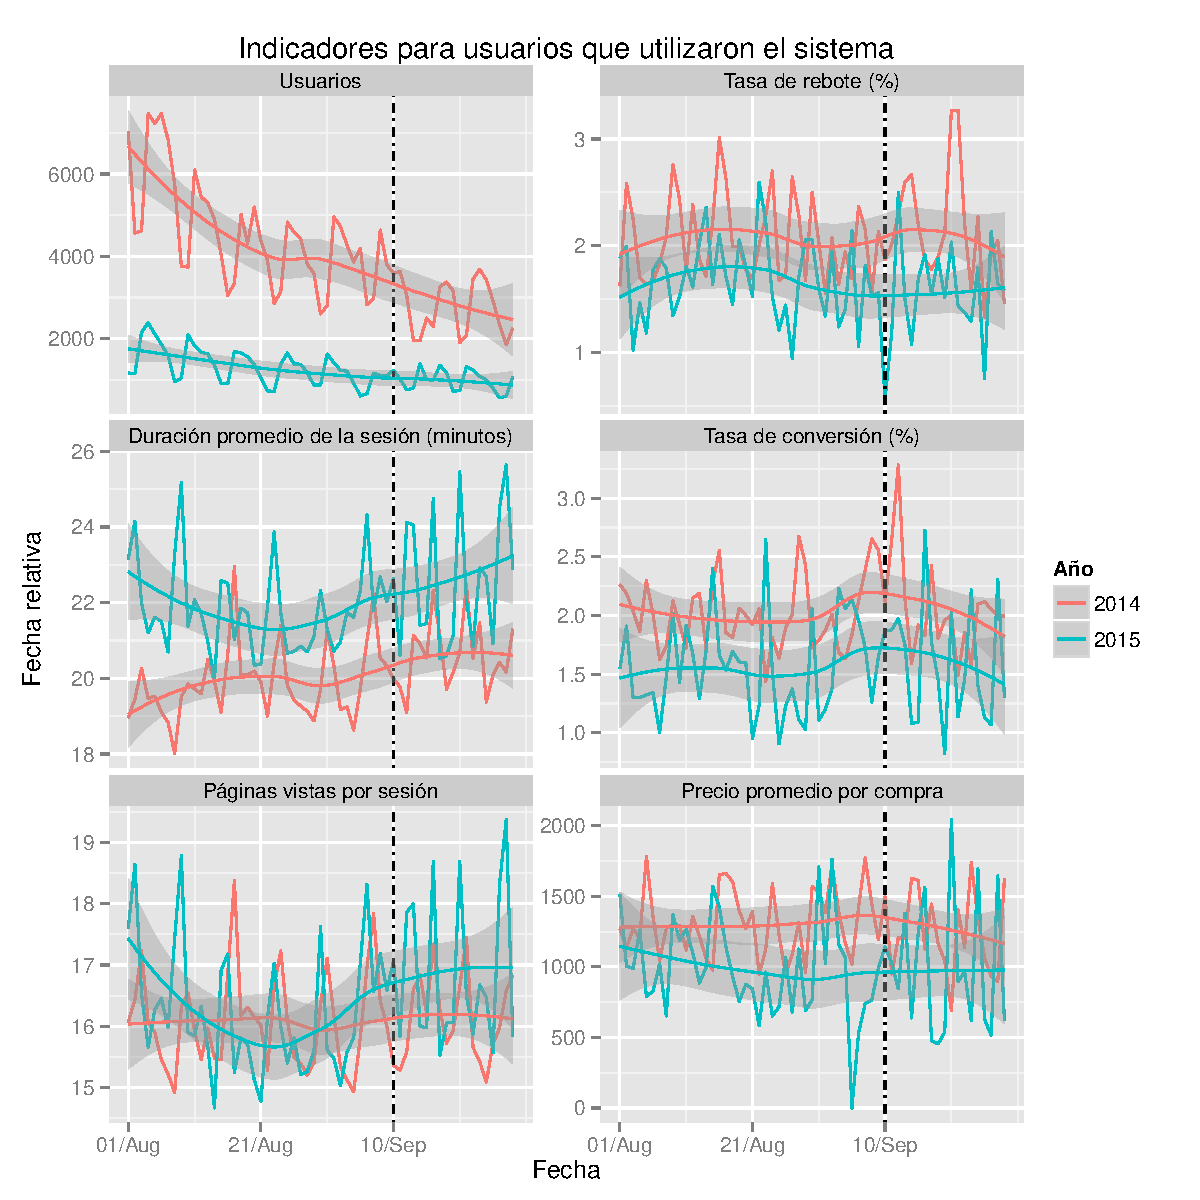
\includegraphics[width=0.9\textwidth]{imagenes/analytics_anios_x.pdf}
	\caption{\label{fig:analytics_x} Métricas del desempeño de la página de agosto y septiembre para 2014 y 2015. La línea vertical indica el momento en el que se cambió el sistema de recomendación en 2015.}
\end{figure}

En la figura (\ref{fig:analytics_x}) podemos ver las series de tiempo de las métricas descritas anteriormente para los años 2014 y 2015. Las líneas punteadas verticales representan el momento de 2015 en el que el sistema nuevo se subió a producción. Si nos fijamos únicamente en las gráficas correspondientes a 2015, es inmediato ver que hay factores estacionales\footnote{Por ejemplo, los usuarios bajan porque hay una transición de temporada alta a temporada baja.} que dificultan la interpretación de las gráficas. Incluimos la información del mismo periodo pero del año anterior (2014) con el fin comparar el comportamiento de los usuarios en la misma época pero sin el sistema nuevo. Desafortunadamente, parece haber factores externos que afectan a las variables. Por ejemplo, el número de usuarios disminuyó fuertemente de un año a otro, incluso antes de la implementación. En ese caso particular sabemos que el cambio se debe a que se movió la lista de recomendaciones a un lugar menos relevante de la página. En general es difícil medir a ciencia cierta el efecto del sistema en las otras variables debido a la enorme variabilidad que presentan. Sin embargo, parece haber un efecto moderado en la duración promedio de las sesiones y las páginas vistas por sesión\footnote{Estas variables están sumamente correlacionadas, así que las contamos dentro del mismo efecto.}. Este hecho es congruente con una mejora en las recomendaciones, pues querría decir que una vez que un cliente comenzó a utilizar el sistema, le gustó más el nuevo que el actual.

A pesar de que obtuvimos algo de información de estas gráficas, el hecho de que son datos muestreados, el ruido que presentan y la influencia de factores externos nos hicieron dudar de nuestras conclusiones. Por ello, consideramos que es prudente preguntarnos si realmente queremos analizar estas métricas, algunas variantes de las mismas o de plano otras completamente nuevas. Una posible respuesta a esto es que hay que modificarlas de modo que revelen su información relevante, puesto que sí son datos apropiados para medir el desempeño de una página web. La transformación que utilizaremos es la siguiente: Supongamos que $X_t$ es uno de los indicadores antes mencionados al tiempo $t$. Entonces, en lugar de $X_t$ utilizaremos el cociente de $X_t$ para las personas que fueron asistidas por el sistema de recomendación (i.e. dieron \emph{click} en alguna recomendación), entre las que no lo utilizaron. Es decir, para un indicador al tiempo $t$, $X_t$, analizaremos
\[
Y_t = \frac{X_t \; | \text{ utilizó el sistema}}{X_t \; | \text{ no utilizó el sistema}}
\]
La ventaja de utilizar $Y_t$ en lugar de $X_t$ es que quita en buena medida los factores externos, por lo que una mala o una buena época no sesgará tan fuertemente los resultados. Esto se debe a que $Y_t$ compara los individuos que utilizaron el sistema con los que no lo usaron, de modo que los factores externos (como por ejemplo un aumento de la cantidad de sesiones en temporada alta) no tendrán efecto alguno, o no uno tan marcado. A pesar de ello, la serie de tiempo $Y_t$ nos indicará si el efecto de $X_t$ ha cambiado para los clientes que utilizaron el sistema en comparación con los demás, desde el momento en que se implementó la nueva versón. Dado que esto último es lo que buscamos averiguar, sí es apropiado utilizar $Y_t$ en lugar de $X_t$. A continuación enlistamos la interpretación de los indicadores transformados:
\begin{enumerate}
	\item Proporción de usuarios que usaron el sistema de recomendación.
	\item Comparación de las \glspl{bouncerate} entre clientes que usaron / no usaron el sistema.
	\item Cociente de duración entre \glspl{sesion} que no usaron el sistema vs. sesiones que sí lo usaron.
	\item 100\% más el porcentaje de veces que aumentó la \gls{conversionrate} al usar el sistema.
	\item 100\% más el aumento porcentual del número de páginas vistas en una sesión.
	\item Cuántas veces más cara es la venta promedio de los usuarios del sistema en comparación con los no usuarios.
\end{enumerate}
En la figura (\ref{fig:analytics_y}) mostramos los indicadores en esta nueva forma, nuevamente para 2014 y 2015. Las conclusiones que podemos sacar de estas gráficas no son tan definitivas como nos gustaría, pero las enunciamos a continuación:
\begin{enumerate}
	\item \emph{Usuarios:} Hubo muchos menos usuarios que usaron el sistema en comparación de los que no en el periodo de observación en 2015 que en 2014. Este hecho probablemente se debe a factores desconocidos como por ejemplo el diseño de la página. Sin embargo, al menos en 2015 la tendencia cambió un poco al momento en que se introdujo el nuevo sistema. Es decir, parece ser que el sistema influyó en que se utilizaran más las recomendaciones, pero hay factores de mucho mayor peso que desconocemos.
	\item \emph{\Gls{bouncerate}:} La \gls{bouncerate} de las personas que utilizan el sistema de recomendación es mucho más baja que la de las que no. En 2015 las \glspl{bouncerate} fueron más bajas que en 2014, pero uno podría esperar que subieran un poco en septiembre (presumiblemente por la temporada). El nuevo sistema parece mitigar ligeramente esta subida, aunque no de forma contundente.
	\item \emph{Duración promedio de la sesión:} Las sesiones de los usuarios del sistema (en comparación con los no-usuarios) eran levemente más cortas en 2014 que en 2015. Analizando los datos del año anterior, se podría esperar que esta variable debería bajar. Sin embargo, en el momento en el que se introdujo el sistema nuevo, siguió en aumento en lugar de bajar, como habría sido de esperarse siguiendo la tendencia de 2014.
	\item \emph{\Gls{conversionrate}:} El cociente de la \gls{conversionrate} entre los usuarios y los no-usuarios se mantuvo aproximandamente igual en los dos años, aunque bajó en 2015. El nuevo sistema no hizo nada definitivo para mejorar este problema, por lo que probablemente depende de otros factores.
	\item \emph{Páginas vistas por sesión:} En este caso tenemos un efecto similar al de la \gls{bouncerate}, puesto que al momento de introducir el nuevo sistema, la tendencia de aumento de este indicador siguió su tendencia lineal en lugar de bajar como lo hizo en 2014.
	\item \emph{Monto promedio por transacción:} Este cociente parece haber mantenido la tendencia que traía, que era un poco más baja que en 2014. Es decir, el sistema nuevo no parece fomentar fuertemente que los clientes compren más caro (\emph{upsell}).
\end{enumerate}
Analizando lo anterior podemos ver varios efectos positivos del sistema. Por ejemplo, el número de páginas visitadas por sesión parece haber aumentado en relación a la tendencia que se esperaría según lo observado en 2014. Es bastante razonable que esto sea el caso, pues si las recomendaciones son mejores y más variadas, aumenta la probabilidad de que un cliente explore más. Otros indicadores de desempeño como la duración de la sesión, la cantidad de páginas vistas por sesión y la \gls{bouncerate} también presentaron mejoras moderadas, en especial las primeras dos. Sin embargo, tal parece que tanto el porcentaje de usuarios que utilizaron el sistema, como la \gls{conversionrate} y el monto de cada compra, no fueron afectados visiblemente por el modelo. El tema de los usuarios probablemente se deba a que el hecho de que un usuario empiece a usar el sistema depende de otros factores más potentes, como la ubicación y el diseño de la lista. Claramente una vez que empiezan a usarlo, sí utilizan más el nuevo que el anterior, como reflejan las páginas vistas por sesión y la duración de las sesiones. Por otro lado, la \gls{conversionrate} y el monto de las compras dependen a fin de cuentas de las ofertas de Best Day. Es decir, por más que un cliente vea más hoteles, no comprará si no está convencido del precio.

La conclusión global de este análisis es que, después de aproximadamente un mes de observación \emph{post} implementación, empezó a haber signos prometedores del nuevo sistema en algunos rubros, pero no en todos. Creemos que para mejorar de manera integral el sistema de recomendación habría que también explorar sus componentes gráficos y otras partes de la página de Best Day. Sin embargo, esos análisis quedan fuera de este trabajo.

\begin{figure}[h!t]
	\centering
	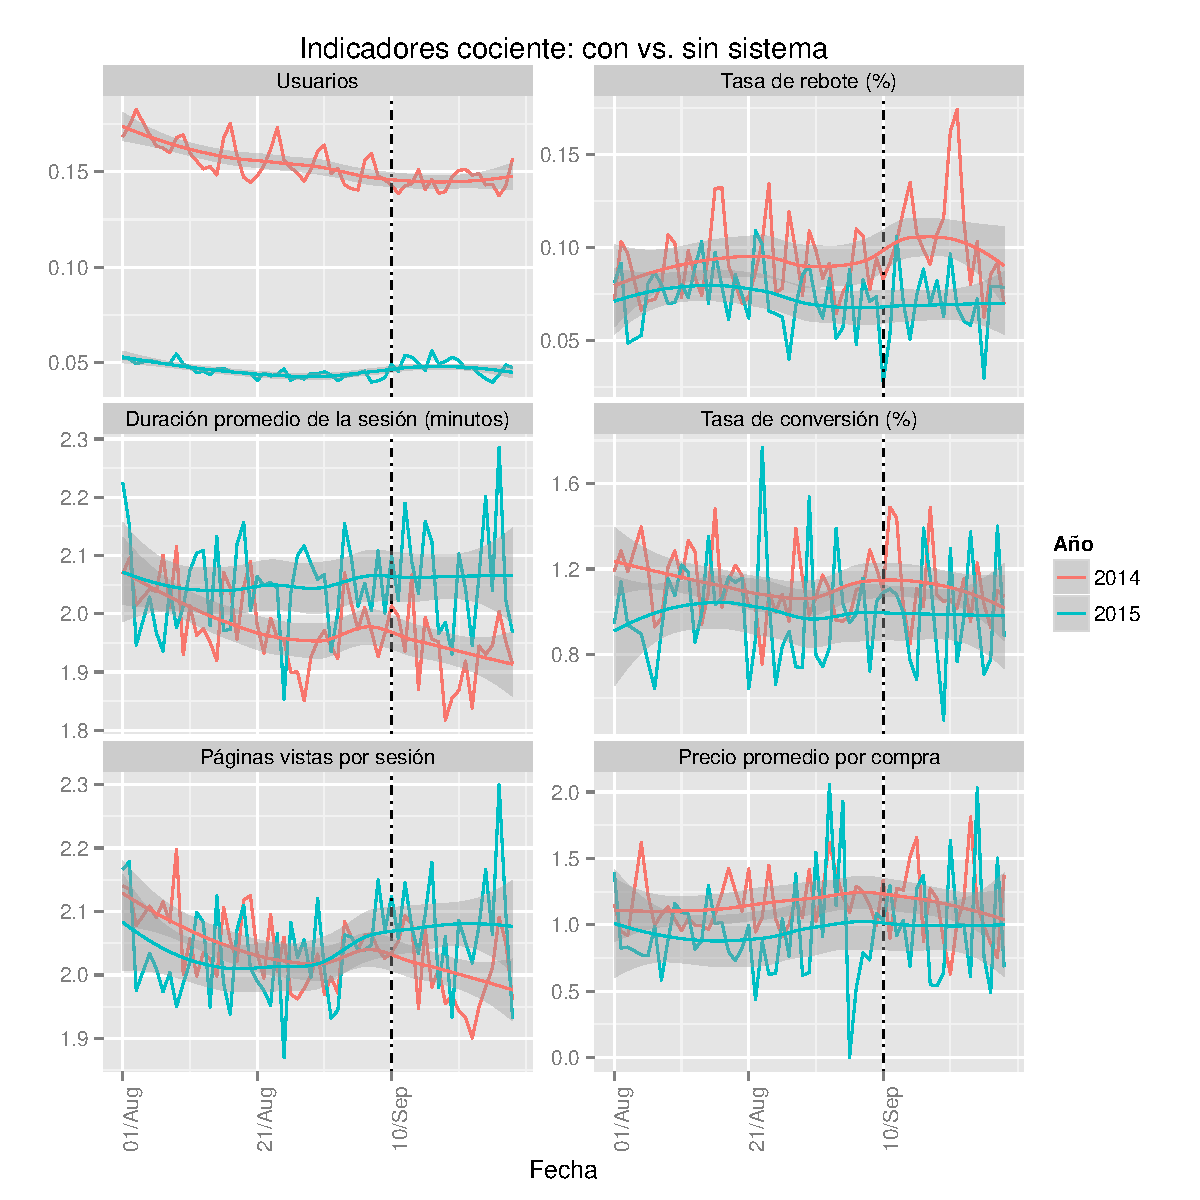
\includegraphics[width=0.9\textwidth]{imagenes/analytics_anios_y.pdf}
	\caption{\label{fig:analytics_y} Indicadores en su forma $Y_t$. La línea vertical indica el momento en el que se cambió el sistema de recomendación.}
\end{figure}


% ----------------------------------------------------------------------------------------------------

\clearpage
\section{Discusión}

Concluiremos el presente trabajo discutiendo algunos temas de interés que surgieron a lo largo del trabajo. Un tema relevante que podría surgir incluso al comenzar a leer esta tesis es \emph{¿por qué utilizamos un sistema de recomendación basado en contenido?} La respuesta esto tiene varias partes. En primer lugar, por razones históricas y de negocio, Best Day no tiene información detallada de todos los clientes\footnote{A diferencia por ejemplo de Netflix o Amazon, que guardan todo el historial de compras y comportamiento de sus clientes.} porque permite comprar viajes sin tener una cuenta con ellos. Aparte de ello, esos sistemas pueden ser más complejos de manejar y se necesita planear antes de implementar la página. Tal como está hoy en día, sería complicado hacerlo sin cambiar varios aspectos estructurales importantes. Además, dado que los viajes son productos caros, los clientes tienen una tasa de compra y de repetición muy bajas, por lo que se contaría con muy poca información por cliente para hacer un filtro colaborativo, por ejemplo. Por estas razones, decidimos que tenía más sentido hacer un sistema no personalizado que tuviera mejores propiedades que el que se tenía inicialmente, pero con la misma premisa de recomendar hoteles similares.

En la parte de teoría hay muchos temas que no están cerrados de ninguna manera. Por ejemplo, uno se podría preguntar \emph{por qué decidimos usar las medidas de verosimilitud como lo hicimos en lugar de distancia coseno}. La respuesta en este caso es que de este modo tenemos una mayor interpretabilidad de los resultados, que perderíamos utilizando distancia coseno o alguna otra medida. Sin embargo, ésta y muchas otras decisiones que tomamos en la construcción del modelo pueden ser fácilmente desafiadas, puesto que, si bien elegimos las mejores opciones que encontramos, no negamos que se pueda encontrar otras mejores. En la sección de trabajo futuro daremos algunas ideas para sofisticar algunos pasos del proceso.

En cuanto al desempeño se refiere, creemos que fue bueno, pero no deslumbrante. Algo que sí logró fue hacernos entender que se requiere mucho más que una buena elección de hoteles para que un sistema de recomendación funcione bien. Es claro que otros aspectos como la presentación y la oferta en sí (que es el producto a fin de cuentas) influyen mucho en la toma de decisiones de los clientes. Un detalle importante que también hay que tener en cuenta sobre este análisis es que los datos de Google Analytics son muestreados. Es decir, dado que hay muchísima información del comportamiento de la página, Google regresa información con una muestra aleatoria con aproximadamente el 20\% del total de la información. Esto podría ocasionar, con mala suerte, que se llegue a conclusiones equivocadas, aunque es sumamente improbable. Otra consideración que hay que tener en este sentido es que, por cuestiones de tiempo, tuvimos menos de un mes de información disponible, y probablemente con un periodo más largo podríamos sacar resultados más definitivos.

Un último tema para esta discusión es que hay que entender los resultados y el desempeño del sistema a la luz de lo que es y de lo que no es. A continuación enlistamos algunos puntos que consideramos de suma importancia para este fin:
\begin{itemize}
	\item \textbf{Qué \emph{sí} hace:}
	\begin{enumerate}
		\item \emph{Recomienda} hoteles similares a uno dado. Tiene una medida de similitud que busca emular el criterio de una persona.
		\item Toma en cuenta el precio con el fin de ser \emph{empático} y atento a las necesidades del cliente.
		\item Toma en cuenta la distancia entre hoteles para que la similitud también sea geográfica.
		\item Intenta emular que es \emph{inteligente} recomendando hoteles de forma no simétrica y no transitiva, con el fin de promover que el cliente \emph{explore} la página.
	\end{enumerate}
	\item \textbf{Qué \emph{no} hace:}
	\begin{enumerate}
		\item No encuentra \glspl{setcompe}\footnote{Ver glosario.} según lo que pensaría una persona, sino según dónde está un hotel y qué ofrece.
		\item No es un sistema de promociones. La versión con precios dinámicos permite que aparezcan hoteles que bajan sus precios en las recomendaciones de hoteles similares más baratos, pero no les da un precio ni un lugar especial.
		\item No toma en cuenta el historial de búsqueda ni es personalizado de ninguna manera.
	\end{enumerate}
\end{itemize}


\section{Trabajo futuro}

En la sección anterior discutimos varios temas interesantes que surgieron en el diseño del modelo. En particular, incluimos una lista de qué hace y qué no hace el sistema que construimos. Nos gustaría concluir este capítulo y el presente trabajo con una lista de las cosas que \emph{podría} hacer el sistema y varias mejoras tecnológicas y visuales que se podría implementar.

Antes que nada, es muy importante notar que encontramos muchos hoteles con información incompleta o sucia, lo que ocasiona que el algoritmo sea menos preciso y no se desempeñe tan bien como podría. Si mejora la calidad y la cantidad de los datos disponibles, el modelo podrá capturar mejor las similitudes entre los hoteles sin hacerle ningún cambio. Sin embargo, hay al menos tres temas que creemos que podría valer la pena investigar. El primero de ellos se refiere a las medidas de similitud. Sería interesante investigarlas ampliamente para ver si tienen algún impacto en la calidad del sistema. Otra idea que se podría explorar es la posibilidad de no tener un porcentaje de precio fijo para el filtro. Pensamos que por ejemplo podría permitirse valores grandes de $\gamma$ para hoteles baratos\footnote{Si un hotel cuesta \$200, uno de \$400 sigue siendo más o menos barato.} y hoteles caros\footnote{Podríamos pensar que el dinero no es problema para ciertos clientes, en cuyo caso habría que recomendar indiscriminadamente la mejor opción.}, pero más pequeños para hoteles de gama media\footnote{En este caso queremos ser más precisos con el precio}. Esto sugeriría que $\gamma$ sea una función del precio del hotel buscado con forma de ``U'' o alguna otra que se encuentre que sea apropiada. Un último cambio que se le podría hacer al modelo es, por ejemplo, tomar en cuenta los hoteles recientemente vistos para recomendar nuevos, aunque esto tendría el riesgo de volver muy rígido al modelo.

Sobre las mejoras tecnológicas, sería útil automatizar la actualización de las recomendaciones, como mencionamos en la sección \ref{sec:arqui}. De este modo, ya no se necesitaría supervisión humana directa para que el sistema corriera, aunque probablemente sería prudente que alguien revisara periódicamente que todo estuviera en orden.

Hablando del desempeño real de la página, el análisis cuantitativo nos llevó a pensar en la enorme magnitud de la influencia que los factores externos tienen sobre el modelo. No podemos enfatizar suficiente que (1) si las recomendaciones son poco atractivas a la vista (en el sentido del diseño de la página), nadie les dará \emph{click} incluso si son excelentes y (2) que, por bien que se recomiende, la conversión no aumentará significativamente si el producto no es suficientemente bueno. Con base en lo anterior y en nuestro criterio, pensamos en varias formas de mejorar el desempeño del sistema como conjunto, más allá del modelo en sí. Una evidente es eliminar al propio hotel de la lista de recomendaciones, con el fin de aprovechar mejor el espacio y así efectivamente lograr que la red de hoteles esté mejor conectada. Otra es que probablemente sería una buena idea poner las recomendaciones en una sección más relevante de la página (por ejemplo arriba a la derecha en lugar de abajor a la derecha) y ponerles un diseño más novedoso. Una última mejora de este tipo podría ser que cuando no haya disponibilidad del hotel buscado, la página muestre las recomendaciones en un lugar prominente, con el fin de presentar hoteles sustitutos de manera conveniente en lugar de obligar al usuario a regresar y buscar de nuevo.







%\glsaddall
%\glossarystyle{altlistgroup}
\printnoidxglossaries


\bibliography{bibliografia}
\bibliographystyle{apalike}
%\bibliographystyle{plain}


\end{document}